% !Mode:: "TeX:UTF-8"
\def\usewhat{dvipdfmx}                              % 定义编译方式 dvipdfmx 或者 pdflatex ,默认为 dvipdfmx
                                                    % 方式编译,如果需要修改,只需改变花括号中的内容即可。
%\setlength{\baselineskip}{20pt}
%\setlength{\headheight}{25pt}
\documentclass[a4paper,12.5pt,openany,twoside]{book}

                                           % 如果论文超过60页 可以使用twoside 双面打印
% !Mode:: "TeX:UTF-8"
%  Authors: 杜家宜   Jiayi Du: Max_dujiayi@gmail.com     湖南大学2010级计算机科学与技术专业博士生

%%%%%%%%%% Package %%%%%%%%%%%%
\usepackage{array}
\newcommand{\PreserveBackslash}[1]{\let\temp=\\#1\let\\=\temp}
\newcolumntype{C}[1]{>{\PreserveBackslash\centering}p{#1}}
\newcolumntype{R}[1]{>{\PreserveBackslash\raggedleft}p{#1}}
\newcolumntype{L}[1]{>{\PreserveBackslash\raggedright}p{#1}}

\usepackage[section]{algorithm}
\usepackage{algorithmic}
\renewcommand{\algorithmicrequire}{\textbf{Input:}}
\renewcommand{\algorithmicensure}{\textbf{Output:}}
\renewcommand{\algorithmiccomment}[1]{\hfill /* #1 */}



\usepackage{graphicx}                       % 支持插图处理
\usepackage{geometry}
\geometry{left=2.5cm,right=2.5cm,top=2cm,bottom=2.5cm,footskip=1.1cm,headsep=0.7cm,head=0.4cm}
                                            % 支持版面尺寸设置
\usepackage{titlesec}                       % 控制标题的宏包
\usepackage{titletoc}                       % 控制目录的宏包
\usepackage{fancyhdr}                       % fancyhdr宏包 支持页眉和页脚的相关定义
\usepackage[UTF8]{ctex}                     % 支持中文显示
\usepackage{color}                          % 支持彩色
\usepackage{amsmath}                        % AMSLaTeX宏包 用来排出更加漂亮的公式
\usepackage{amssymb}                        % 数学符号生成命令
\usepackage[below]{placeins}                %允许上一个section的浮动图形出现在下一个section的开始部分,还提供\FloatBarrier命令,使所有未处理的浮动图形立即被处理
\usepackage{flafter}                        % 使得所有浮动体不能被放置在其浮动环境之前,以免浮动体在引述它的文本之前出现.
\usepackage{multirow}                       % 使用Multirow宏包,使得表格可以合并多个row格
\usepackage{booktabs}                       % 表格,横的粗线;\specialrule{1pt}{0pt}{0pt}
\usepackage{longtable}                      % 支持跨页的表格。
\usepackage{tabularx}                       % 自动设置表格的列宽
\usepackage{setspace}
\usepackage{subfigure}                      % 支持子图 %centerlast 设置最后一行是否居中
\usepackage[subfigure]{ccaption}            % 支持子图的中文标题
\usepackage[sort&compress,numbers]{natbib}  % 支持引用缩写的宏包
\usepackage{enumitem}                       % 使用enumitem宏包,改变列表项的格式
\usepackage{calc}                           % 长度可以用+ - * / 进行计算
\usepackage{txfonts}                        % 字体宏包
\usepackage{bm}                             % 处理数学公式中的黑斜体的宏包
\usepackage[amsmath,thmmarks,hyperref]{ntheorem}  % 定理类环境宏包,其中 amsmath 选项用来兼容 AMS LaTeX 的宏包
\usepackage{CJKnumb}                        % 提供将阿拉伯数字转换成中文数字的命令
\usepackage{indentfirst}                    % 首行缩进宏包
\usepackage{CJKutf8}                        % 用在UTF8编码环境下,它可以自动调用CJK,同时针对UTF8编码作了设置。
\usepackage{CJK}
\usepackage{fancyhdr}
\usepackage{lastpage}
\usepackage{layout}
\usepackage[titles,subfigure]{tocloft}                       %控制生成的表格和图片的目录格式

%\usepackage{hypbmsec}                      % 用来控制书签中标题显示内容

%如果您的pdf制作中文书签有乱码使用如下命令,就可以解决了
\usepackage[dvipdfm, unicode,               % pdflatex, pdftex 这里决定运行文件的方式不同
            pdfstartview=FitH,
            %CJKbookmarks=true,
            bookmarksnumbered=true,
            bookmarksopen=true,
            colorlinks=true,
            pdfborder={0 0 1},
            citecolor=black,
            linkcolor=black,
            anchorcolor=black,
            urlcolor=black,
            breaklinks=true
            ]{hyperref}


                      % 定义本文所使用宏包
\graphicspath{{figures/}}                  % 定义所有的.eps文件在figures子目录下
\begin{document}                           % 开始全文
\begin{CJK*}{UTF8}{song}                   % 开始中文字体使用
% !Mode:: "TeX:UTF-8"
%  Authors: 杜家宜   Jiayi Du: Max_dujiayi@gmail.com     湖南大学2010级计算机科学与技术专业博士生

%%%%%%%%%% Fonts Definition and Basics %%%%%%%%%%%%%%%%%
\newcommand{\song}{\CJKfamily{song}}    % 宋体
\newcommand{\fs}{\CJKfamily{fs}}        % 仿宋体
\newcommand{\kai}{\CJKfamily{kai}}      % 楷体
\newcommand{\hei}{\CJKfamily{hei}}      % 黑体
\newcommand{\li}{\CJKfamily{li}}        % 隶书
\newcommand{\yihao}{\fontsize{26pt}{26pt}\selectfont}       % 一号, 1.倍行距
\newcommand{\xiaoyi}{\fontsize{24pt}{24pt}\selectfont}      % 小一, 1.倍行距
\newcommand{\erhao}{\fontsize{22pt}{22pt}\selectfont}       % 二号, 1.倍行距
\newcommand{\xiaoer}{\fontsize{18pt}{18pt}\selectfont}      % 小二, 单倍行距
\newcommand{\sanhao}{\fontsize{16pt}{16pt}\selectfont}      % 三号, 1.倍行距
\newcommand{\xiaosan}{\fontsize{15pt}{15pt}\selectfont}     % 小三, 1.倍行距
\newcommand{\sihao}{\fontsize{14pt}{14pt}\selectfont}       % 四号, 1.0倍行距
\newcommand{\xiaosi}{\fontsize{12.5pt}{12.5pt}\selectfont}      % 小四, 1.倍行距
\newcommand{\wuhao}{\fontsize{10.5pt}{10.5pt}\selectfont}   % 五号, 单倍行距
\newcommand{\xiaowu}{\fontsize{9pt}{9pt}\selectfont}        % 小五, 单倍行距
\setlength{\headheight}{20pt} 
%\CJKcaption{gb_452}
\CJKtilde  % 重新定义了波浪符~的意义
\newcommand\prechaptername{第}
\newcommand\postchaptername{章}

% 调整罗列环境的布局
\setitemize{leftmargin=3em,itemsep=0em,partopsep=0em,parsep=0em,topsep=-0em}
\setenumerate{leftmargin=3em,itemsep=0em,partopsep=0em,parsep=0em,topsep=0em}


%避免宏包 hyperref 和 arydshln 不兼容带来的目录链接失效的问题。
\def\temp{\relax}
\let\temp\addcontentsline
\gdef\addcontentsline{\phantomsection\temp}

% 自定义项目列表标签及格式 \begin{publist} 列表项 \end{publist}
\newcounter{pubctr} %自定义新计数器
\newenvironment{publist}{%%%%%定义新环境
\begin{list}{[\arabic{pubctr}]} %%标签格式
    {
     \usecounter{pubctr}
     \setlength{\leftmargin}{2.5em}     % 左边界 \leftmargin =\itemindent + \labelwidth + \labelsep
     \setlength{\itemindent}{0em}     % 标号缩进量
     \setlength{\labelsep}{1em}       % 标号和列表项之间的距离,默认0.5em
     \setlength{\rightmargin}{0em}    % 右边界
     \setlength{\topsep}{0ex}         % 列表到上下文的垂直距离
     \setlength{\parsep}{0ex}         % 段落间距
     \setlength{\itemsep}{0ex}        % 标签间距
     \setlength{\listparindent}{0pt} % 段落缩进量
    }}
{\end{list}}%%%%%


\makeatletter
\renewcommand\normalsize{
  \@setfontsize\normalsize{12.5pt}{12.5pt} % 小四对应12pt
  \setlength\abovedisplayskip{4pt}
  \setlength\abovedisplayshortskip{4pt}
  \setlength\belowdisplayskip{\abovedisplayskip}
  \setlength\belowdisplayshortskip{\abovedisplayshortskip}
    \let\@listi\@listI}
\def\defaultfont{\renewcommand{\baselinestretch}{1.65}\normalsize\selectfont}


% 设置行距和段落间垂直距离

\setlength{\baselineskip}{20pt}
\renewcommand{\CJKglue}{\hskip 0.5pt plus \baselineskip} %加大字间距,使每行35个字


\makeatother

%%%%%%%%%%%%% Contents %%%%%%%%%%%%%%%%%
\renewcommand{\contentsname}{目\qquad 录}
\setcounter{tocdepth}{2}
\titlecontents{chapter}[1em]{\xiaosi\hei}%
             {\prechaptername~~\thecontentslabel~~\postchaptername~~~}{} %
             {\titlerule*[5pt]{$\cdot$}\xiaosi\contentspage}
\titlecontents{section}[3em]{\xiaosi\song} %
            {\thecontentslabel\quad}{} %
            {\hspace{.25em}\titlerule*[5pt]{$\cdot$}\xiaosi\contentspage}
\titlecontents{subsection}[4em]{\xiaosi\song} %
            {\thecontentslabel\quad}{} %
            {\hspace{.25em}\titlerule*[5pt]{$\cdot$}\xiaosi\contentspage}
\renewcommand{\cftdotsep}{1.1}
\renewcommand{\listfigurename}{插图索引}
\setcounter{lofdepth}{1}
%\titlefigures{chapter}[1em]{\xiaosi\hei}%
             %{\prechaptername~~\thecontentslabel~~\postchaptername~~~}{} %
            % {\titlerule*[10pt]{$\cdot$}\xiaosi\contentspage}
\renewcommand{\listtablename}{附表索引}



%%删除表格和插图因章不同中的空行%%%
\makeatletter
\def\@chapter[#1]#2{\ifnum \c@secnumdepth >\m@ne
                       \if@mainmatter
                         \refstepcounter{chapter}%
                         \typeout{\@chapapp\space\thechapter.}%
                         \addcontentsline{toc}{chapter}%
                                   {\protect\numberline{\thechapter}#1}%
                       \else
                         \addcontentsline{toc}{chapter}{#1}%
                       \fi
                    \else
                      \addcontentsline{toc}{chapter}{#1}%
                    \fi
                    \chaptermark{#1}%
                    \if@twocolumn
                      \@topnewpage[\@makechapterhead{#2}]%
                    \else
                      \@makechapterhead{#2}%
                      \@afterheading
                    \fi}
\makeatother


%%%%%%%%%% Chapter and Section %%%%%%%%%%%%%%%%%
\setcounter{secnumdepth}{4}
\setlength{\parindent}{2em}
\renewcommand{\chaptername}{\prechaptername\arabic{chapter}\postchaptername}
\titleformat{\chapter}{\centering\xiaoer\hei}{\chaptername}{1em}{}
\titlespacing{\chapter}{0pt}{0pt}{18pt}
\titleformat{\section}{\xiaosan\hei}{\thesection}{1em}{}
\titlespacing{\section}{0pt}{12pt}{12pt}
\titleformat{\subsection}{\sihao\hei}{\thesubsection}{0.5em}{}
\titlespacing{\subsection}{0pt}{6pt}{6pt}
\titleformat{\subsubsection}{\xiaosi\hei}{\thesubsubsection}{0.5em}{}
\titlespacing{\subsubsection}{0pt}{6pt}{6pt}

%%%%%%%%%% Table, Figure and Equation %%%%%%%%%%%%%%%%%
\renewcommand{\tablename}{表} % 插表题头
\renewcommand{\figurename}{图} % 插图题头
\renewcommand{\thefigure}{\arabic{chapter}.\arabic{figure}} % 使图编号为 7.1 的格式 %\protect{~}
\renewcommand{\thetable}{\arabic{chapter}.\arabic{table}}%使表编号为 7.1 的格式
\renewcommand{\theequation}{\arabic{chapter}.\arabic{equation}}%使公式编号为 7-1 的格式
\renewcommand{\thesubfigure}{(\alph{subfigure})}%使子图编号为 (a)的格式
\renewcommand{\thesubtable}{(\alph{subtable})} %使子表编号为 (a)的格式
\makeatletter
\renewcommand{\p@subfigure}{\thefigure~} %使子图引用为 7-1 a) 的格式,母图编号和子图编号之间用~加一个空格
\makeatother


%% 定制浮动图形和表格标题样式
\makeatletter
\long\def\@makecaption#1#2{%
   \vskip\abovecaptionskip
   \sbox\@tempboxa{\centering\wuhao\hei{#1~~#2} }%
   \ifdim \wd\@tempboxa >\hsize
     \centering\wuhao\hei{#1~~#2} \par
   \else
     \global \@minipagefalse
     \hb@xt@\hsize{\hfil\box\@tempboxa\hfil}%
   \fi
   \vskip\belowcaptionskip}
\makeatother
\captiondelim{~~~~} %用来控制longtable表头分隔符

%%%%%%%%%% Theorem Environment %%%%%%%%%%%%%%%%%
\theoremstyle{plain}
\theorembodyfont{\song\rmfamily}
\theoremheaderfont{\hei\rmfamily}
\newtheorem{theorem}{定理~}[chapter]
\newtheorem{lemma}{引理~}[chapter]
\newtheorem{axiom}{公理~}[chapter]
\newtheorem{proposition}{命题~}[chapter]
\newtheorem{corollary}{推论~}[chapter]
\newtheorem{definition}{定义~}[chapter]
\newtheorem{conjecture}{猜想~}[chapter]
\newtheorem{example}{例~}[chapter]
\newtheorem{remark}{注~}[chapter]
\floatname{algorithm}{算法}%将英文的algorithm改为算法
\renewcommand{\algorithmicrequire}{\textbf{Input:}}
\renewcommand{\algorithmicensure}{\textbf{Output:}}
\newenvironment{proof}{\noindent{\hei 证明:}}{\hfill $ \square $ \vskip 4mm}
\theoremsymbol{$\square$}

%%%%%%%%%% Page: number, header and footer  页码%%%%%%%%%%%%%%%%%

%\frontmatter 或 \pagenumbering{roman}
%\mainmatter 或 \pagenumbering{arabic}
\makeatletter
\renewcommand\frontmatter{\clearpage
  \@mainmatterfalse
  \pagenumbering{Roman}} % 正文前罗马字体编号
\makeatother


%%%%%%%%%% References %%%%%%%%%%%%%%%%%
\renewcommand{\bibname}{参考文献}
% 重定义参考文献样式,来自thu
\makeatletter
\renewenvironment{thebibliography}[1]{%
   \chapter*{\bibname}%
   \xiaosi
   \list{\@biblabel{\@arabic\c@enumiv}}%
        {\renewcommand{\makelabel}[1]{##1\hfill}
         \setlength{\baselineskip}{21pt}
         \settowidth\labelwidth{0.5cm}
         \setlength{\labelsep}{0pt}
         \setlength{\itemindent}{0pt}
         \setlength{\leftmargin}{\labelwidth+\labelsep}
         \addtolength{\itemsep}{-0.7em}
         \usecounter{enumiv}%
         \let\p@enumiv\@empty
         \renewcommand\theenumiv{\@arabic\c@enumiv}}%
    \sloppy\frenchspacing
    \clubpenalty4000%
    \@clubpenalty \clubpenalty
    \widowpenalty4000%
    \interlinepenalty4000%
    \sfcode`\.\@m}
   {\def\@noitemerr
     {\@latex@warning{Empty `thebibliography' environment}}%
    \endlist\frenchspacing}
\makeatother

\addtolength{\bibsep}{5pt} % 增加参考文献间的垂直间距
\setlength{\bibhang}{2em} %每个条目自第二行起缩进的距离

% 参考文献引用作为上标出现
\newcommand{\mycite}[1]{\scalebox{1.3}[1.3]{\raisebox{-0.65ex}{\cite{#1}}}}

%% 引用格式
\bibpunct{[}{]}{,}{s}{}{,}

%%%%%%%%%% Cover %%%%%%%%%%%%%%%%%
% 封面、摘要、版权、致谢格式定义
\makeatletter

%\def\dtitle#1{\def\@dtitle{#1}}\def\@dtitle{}
\def\ctitle#1{\def\@ctitle{#1}}\def\@ctitle{}
\def\etitle#1{\def\@etitle{#1}}\def\@etitle{}
\def\caffil#1{\def\@caffil{#1}}\def\@caffil{}
\def\cmacrosubject#1{\def\@cmacrosubject{#1}}\def\@cmacrosubject{}
\def\cmacrosubjecttitle#1{\def\@cmacrosubjecttitle{#1}}\def\@cmacrosubjecttitle{}
\def\csubject#1{\def\@csubject{#1}}\def\@csubject{}
\def\csubjecttitle#1{\def\@csubjecttitle{#1}}\def\@csubjecttitle{}
\def\cmajor#1{\def\@cmajor{#1}}\def\@cmajor{}
\def\cauthor#1{\def\@cauthor{#1}}\def\@cauthor{}
\def\cauthortitle#1{\def\@cauthortitle{#1}}\def\@cauthortitle{}
\def\csupervisor#1{\def\@csupervisor{#1}}\def\@csupervisor{}
\def\csupervisortitle#1{\def\@csupervisortitle{#1}}\def\@csupervisortitle{}
\def\cdate#1{\def\@cdate{#1}}\def\@cdate{}
\def\untitle#1{\def\@untitle{#1}}\def\@untitle{}
\def\declaretitle#1{\def\@declaretitle{#1}}\def\@declaretitle{}
\def\declarecontent#1{\def\@declarecontent{#1}}\def\@declarecontent{}
\def\authorizationtitle#1{\def\@authorizationtitle{#1}}\def\@authorizationtitle{}
\def\authorizationcontent#1{\def\@authorizationcontent{#1}}\def\@authorizationconent{}
\def\authorizationadd#1{\def\@authorizationadd{#1}}\def\@authorizationadd{}
\def\authorsigncap#1{\def\@authorsigncap{#1}}\def\@authorsigncap{}
\def\supervisorsigncap#1{\def\@supervisorsigncap{#1}}\def\@supervisorsigncap{}
\def\signdatecap#1{\def\@signdatecap{#1}}\def\@signdatecap{}
\long\def\cabstract#1{\long\def\@cabstract{#1}}\long\def\@cabstract{}
\long\def\eabstract#1{\long\def\@eabstract{#1}}\long\def\@eabstract{}
\def\ckeywords#1{\def\@ckeywords{#1}}\def\@ckeywords{}
\def\ekeywords#1{\def\@ekeywords{#1}}\def\@ekeywords{}
\def\cheading#1{\def\@cheading{#1}}\def\@cheading{}
\def\cnumber#1{\def\@cnumber{#1}}\def\@cnumber{}
\def\csecret#1{\def\@csecret{#1}}\def\@csecret{}
\def\chnunumer#1{\def\@chnunumer{#1}}\def\@chnunumer{}
\def\cclassnumber#1{\def\@cclassnumber{#1}}\def\@cclassnumber{}
\def\chnuname#1{\def\@chnuname{#1}}\def\@chnuname{}
\def\cchair#1{\def\@cchair{#1}}\def\@cchair{}
\def\ddate#1{\def\@ddate{#1}}\def\@ddate{}
%英文内封
\def\ename#1{\def\@ename{#1}}\def\@ename{}
\def\cbe#1{\def\@cbe{#1}}\def\@cbe{}
%\def\cms#1{\def\@cms{#1}}\def\@cms{}
\def\cdegree#1{\def\@cdegree{#1}}\def\@cdegree{}
\def\cclass#1{\def\@cclass{#1}}\def\@cclass{}
\def\emajor#1{\def\@emajor{#1}}\def\@emajor{}
\def\ehnu#1{\def\@ehnu{#1}}\def\@ehnu{}
\def\esupervisor#1{\def\@esupervisor{#1}}\def\@esupervisor{}
\def\edate#1{\def\@edate{#1}}\def\@edate{}



\newlength{\@title@width}
\def\@put@covertitle#1{\makebox[\@title@width][s]{#1}}
% 定义封面
\def\makecover{
%\cleardoublepage%
  \phantomsection
  \pdfbookmark[-1]{\@ctitle}{ctitle}

  \begin{titlepage}
  \begin{center}

    \setlength{\@title@width}{3.5cm}
    {
      \begin{tabular}{lcclc}
        \xiaosi\hei{学校代号}&  \underline{\makebox[\@title@width][c]{\@chnunumer}}&\qquad \qquad \qquad \qquad \qquad & \xiaosi\hei{学\qquad 号}&  \underline{\makebox[\@title@width][c]{\@cnumber}}\\
        \xiaosi\hei{分~~类~~~号}&  \underline{\makebox[\@title@width][c]{\@cclassnumber}}&\qquad \qquad \qquad \qquad \qquad & \xiaosi\hei{密\qquad 级}&  \underline{\makebox[\@title@width][c]{\@csecret}} \\
      \end{tabular}
    }

    \begin{figure}[h]
      \centering
      
\includegraphics[width=0.3\textwidth]{figures/Hnulogo}
    \end{figure}

    \vspace*{1cm}{\hei\erhao \@cheading}

    \vspace*{1cm}


    \begin{center}
      \begin{spacing}{1.5}
        \hei\yihao \@ctitle
      \end{spacing}
    \end{center}

    \vspace{\baselineskip}

    \setlength{\@title@width}{6.8cm}
    {

      \begin{spacing}{2.1}
        \xiaosi\hei{学位申请人姓名} \xiaosi\song\underline{\makebox[\@title@width][l]{\quad\@cauthor}} \\
        \xiaosi\hei{培~~~~养~~~~~单~~~~~位} \xiaosi\song\underline{\makebox[\@title@width][l]{\quad\@caffil}} \\
        \xiaosi\hei{导师姓名及职称} \xiaosi\song\underline{\makebox[\@title@width][l]{\quad\@csupervisor}} \\
        \xiaosi\hei{学~~~~科~~~~~专~~~~~业} \xiaosi\song\underline{\makebox[\@title@width][l]{\quad\@csubject}} \\
        \xiaosi\hei{研~~~~究~~~~~方~~~~~向} \xiaosi\song\underline{\makebox[\@title@width][l]{\quad\@cmajor}}\\
        \xiaosi\hei{论~文~提~交~日~~期} \xiaosi\song\underline{\makebox[\@title@width][l]{\quad\@cdate}} \\
        %\end{tabular}
      \end{spacing}
    }
  \end{center}


  \clearpage
  \thispagestyle{empty} %去掉页眉页脚

  \noindent
  \makebox[2.59cm][s]{}{
    \begin{tabular}{ll}
      \xiaosi\hei 学校代号:\xiaosi\song~~\@chnunumer \\
      \xiaosi\hei 学\qquad~号:\xiaosi\song~~\@cnumber\\
      \xiaosi\hei 密\qquad~级:\xiaosi\song~~\@csecret\\
    \end{tabular}
  }

%
  \vspace{5\baselineskip}

  \noindent
  \makebox[2.59cm][s]{}{
    \xiaoer\song \@chnuname \@cheading
  }
 % \\
  \vspace{4\baselineskip}

  \begin{spacing}{2}
    \hangafter=1\hangindent=2.7cm   %换行后自动缩进
    {
      \noindent
      \makebox[2.59cm][s]{} {\hei\erhao\@ctitle}
    }

  \end{spacing}

  \vspace{4\baselineskip}

  \setlength{\@title@width}{6.8cm}
  {
    \begin{spacing}{2}
      \noindent
      \makebox[2.59cm][s]{}
      {
        \begin{tabular}{lc}
         \underline{\xiaosi\hei学位申请人姓名:\song\makebox[\@title@width][l]{\qquad\qquad\@cauthor}} \\
         \underline{\xiaosi\hei导师姓名及职称:\song\makebox[\@title@width][l]{\qquad\qquad\@csupervisor}} \\
         \underline{\xiaosi\hei培~~~~养~~~~~单~~~~位:\song\makebox[\@title@width][l]{\qquad\qquad\@caffil}} \\
         \underline{\xiaosi\hei专~~~~业~~~~~名~~~~称:\song\makebox[\@title@width][l]{\qquad\qquad\@csubject}} \\
         \underline{\xiaosi\hei论~文~提~交~日~期:\song\makebox[\@title@width][l]{\qquad\qquad\@cdate}} \\
         \underline{\xiaosi\hei论~文~答~辩~日~期:\song\makebox[\@title@width][l]{\qquad\qquad\@ddate}}\\
         \underline{\xiaosi\hei答辩委员会主席:\song\makebox[\@title@width][l]{\qquad\qquad\@cchair}} \\
        \end{tabular}
        
      }
   \end{spacing}
  }

  \clearpage
  \thispagestyle{empty} %去掉页眉页脚

  \begin{center}
    \qquad\\
    \begin{spacing}{2.5}
      \xiaosan \@etitle
    \end{spacing}



    \begin{spacing}{2}
       \xiaosi
       by\\
       \@ename \\
       \@cbe\\
      % \@cms\\
       A~\@cdegree~submitted in partial satisfaction of the\\
       requirements for the degree of\\
       \@cclass\\
       in\\
      \@emajor\\
      in the\\
      Graduate school\\
       of\\
       \@ehnu\\

       \vspace{2\baselineskip}

      Supervisor\\
      Professor \@esupervisor\\
      \@edate
    \end{spacing}

  \end{center}


\end{titlepage}

%  另起一页: 独创性声明和学位论文版权使用授权书

\pagestyle{fancy}
\fancyhf{}
\fancyfoot[C]{\song\xiaowu ~\thepage~}
\renewcommand{\headrulewidth}{0pt}

    \addcontentsline{toc}{chapter}{学位论文原创性声明和学位论文版权使用授权书}{
    \setcounter{page}{1}
    \qquad\\
    \begin{center}\hei\xiaoer{\@untitle}\end{center}\par
    \begin{center}\hei\xiaoer{\@declaretitle}\end{center}\par
    \song\defaultfont{\@declarecontent}\par
    \vspace*{1cm}
    {\song\xiaosi
    \@authorsigncap \makebox[2.5cm][s]{}
    \@signdatecap \makebox[2cm][s]{} 年 \makebox[1cm][s]{} 月 \makebox[1cm][s]{} 日
    }
    \vspace{0.6\baselineskip}
    \begin{center}\hei\xiaoer{\@authorizationtitle}\end{center}\par
    {
    \vspace{1.2\baselineskip}
    \song\defaultfont{\@authorizationcontent}
    \begin{tabular}{ll}
     \song\defaultfont\@authorizationadd\par&\\
    &1、保密\song\xiaoer{$\Box$}\song\xiaosi ,在\underline{\qquad}年解密后适用于本授权书\\
    &2、不保密。\\
    &(请在以上相应方框内打"$\surd$") \\
    \end{tabular}
    }
    \vspace{2\baselineskip}

    {
    \song\xiaosi
      \@authorsigncap \makebox[3.5cm][s]{}  \@signdatecap \makebox[1.5cm][s]{} 年 \makebox[1cm][s]{} 月 \makebox[1cm][s]{} 日 \\
      \indent
      \@supervisorsigncap \makebox[3.5cm][s]{}  \@signdatecap \makebox[1.5cm][s]{} 年 \makebox[1cm][s]{} 月 \makebox[1cm][s]{} 日
    }
    }


%%%%%%%%%%%%%%%%%%%   Abstract and Keywords  %%%%%%%%%%%%%%%%%%%%%%%
\clearpage

\pagestyle{fancy}
  \fancyhf{}
\fancyhead[CO]{\song\xiaowu \@cheading}
\fancyhead[CE]{\song\xiaowu \@ctitle}
\fancyfoot[C]{\song\xiaowu ~\thepage~}
\makeatletter %双线页眉
\def\headrule{{\if@fancyplain\let\headrulewidth\plainheadrulewidth\fi%
\hrule\@height 1.0pt \@width\headwidth\vskip1pt %上面线为1pt粗
\hrule\@height 0.5pt\@width\headwidth  %下面0.5pt粗
\vskip-2\headrulewidth\vskip-1pt}      %两条线的距离1pt
\vspace{7mm} %双线与下面正文之间的垂直间距
}

\fancypagestyle{plain}{% 设置开章页页眉页脚风格
    \fancyhf{}%
\fancyhead[CO]{\song\xiaowu \@cheading}
\fancyhead[CE]{\song\xiaowu \@ctitle}
\fancyfoot[C]{\song\xiaowu ~\thepage~} %首页页脚格式
%双线页眉的设置
\makeatletter %双线页眉
\def\headrule{{\if@fancyplain\let\headrulewidth\plainheadrulewidth\fi%
\hrule\@height 1.0pt \@width\headwidth\vskip1pt %上面线为1pt粗
\hrule\@height 0.5pt\@width\headwidth  %下面0.5pt粗
\vskip-2\headrulewidth\vskip-1pt}      %两条线的距离1pt
\vspace{7mm} %双线与下面正文之间的垂直间距
}

}
\addcontentsline{toc}{chapter}{摘~要}
\chapter*{\centering\xiaoer\ 摘\qquad 要}
\song\defaultfont
\@cabstract
\vspace{\baselineskip}

%\hangafter=1\hangindent=52.3pt\noindent   %如果取消该行注释,关键词换行时将会自动缩进
\noindent
{\hei\xiaosi 关键词: \@ckeywords}

%%%%%%%%%%%%%%%%%%%   English Abstract  %%%%%%%%%%%%%%%%%%%%%%%%%%%%%%
\clearpage

\addcontentsline{toc}{chapter}{Abstract}
\chapter*{\centering\xiaoer \bf{Abstract}}
%\vspace{\baselineskip}
\@eabstract
\vspace{\baselineskip}

%\hangafter=1\hangindent=60pt\noindent  %如果取消该行注释,KEY WORDS换行时将会自动缩进
\noindent
{\xiaosi\bf{Key Words: \@ekeywords}}
}
\clearpage
\makeatother
                       % 完成对论文各个部分格式的设置
\frontmatter                               % 以下是论文导言部分,包括论文的封面,中英文摘要和中文目录
% !Mode:: "TeX:UTF-8"

\chnunumer{10532}
\chnuname{湖南大学}
\cclassnumber{TP391}
\cnumber{~~~~~}
\csecret{普通}
\cmajor{大规模图计算}
\cheading{硕士学位论文}      % 设置正文的页眉,以及自己的学位级别
\ctitle{基于单机多核系统的图处理研究}  %封面用论文标题,自己可手动断行
\etitle{Graph Processing Research on Single Multi-core Systems}
\caffil{信息科学与工程学院} %学院名称
\csubjecttitle{学科专业}
\csubject{计算机科学与技术}   %专业
\cauthortitle{研究生}     % 学位
\cauthor{~~~}   %学生姓名
\ename{~~~~}
\cbe{B.E.~(Hunan University)~2015}
%\cms{M.S.~(Hunan University)2010}
\cdegree{thesis}
\cclass{Master of engineering}
\emajor{Computer Science and Technology}
\ehnu{Hunan~University}
\esupervisor{~~}
\csupervisortitle{指导教师}
\csupervisor{~~~教授} %导师姓名
\cchair{~~~~~~~~}
\ddate{~~~~~~~~年~~~~月~~~~日}
\edate{April,~2014}

\untitle{湖~~南~~大~~学}
\declaretitle{学位论文原创性声明}
\declarecontent{
本人郑重声明:所呈交的论文是本人在导师的指导下独立进行研究所取得的研究成果。除了文中特别加以标注引用的内容外,本论文不包含任何其他个人或集体已经发表或撰写的成果作品。对本文的研究做出重要贡献的个人和集体,均已在文中以明确方式标明。本人完全意识到本声明的法律后果由本人承担。
}
\authorizationtitle{学位论文版权使用授权书}
\authorizationcontent{
本学位论文作者完全了解学校有关保留、使用学位论文的规定,同意学校保留并向国家有关部门或机构送交论文的复印件和电子版,允许论文被查阅和借阅。本人授权湖南大学可以将本学位论文的全部或部分内容编入有关数据库进行检索,可以采用影印、缩印或扫描等复制手段保存和汇编本学位论文。
}
\authorizationadd{本学位论文属于}
\authorsigncap{作者签名:}
\supervisorsigncap{导师签名:}
\signdatecap{签字日期:}


%\cdate{\CJKdigits{\the\year} 年\CJKnumber{\the\month} 月 \CJKnumber{\the\day} 日}
% 如需改成二零一二年四月二十五日的格式,可以直接输入,即如下所示
% \cdate{二零一二年四月二十五日}
\cdate{~~~~~~~~年~~~~月~~~~日} % 此日期显示格式为阿拉伯数字 如2012年4月25日
\cabstract{

随着各种类型的社交网络的兴起,基于图结构数据的企业级应用正变得日益广泛与重要。而如何高效便捷的分析、调试和处理这些与日俱增的大规模图数据成为当前高性能计算领域的研究人员所面临的最迫切的问题之一。目前,已经存在一些解决方案,但是这些解决方案还存在着一定的问题。例如,分布式解决方案中存在着负载均衡、通信延迟以及经济成本高的问题,而单机系统的解决方案则存在着并发度低,容错性差等问题。本文从兼容性、容错性与便捷高效的角度考虑,提出了基于并行BSP模型的单机图处理系统GPSA(Graph Processing System with Actors)。首先,GPSA使用Actor的并发模型改善系统的并发性和计算吞吐量。Actor模型不仅充分的利用多核的优势,同时避免频繁的上下文的切换所带来的性能损耗;其次,改进传统的BSP计算模型。基于BSP模型的图处理过程主要有计算和消息分发两个步骤。在传统的BSP模型中,由于图数据的局部性问题,在以顶点为中心的实现方式中单个顶点上的计算和通信两个步骤需要顺序执行。GPSA结合Actor与BSP模型将图计算中顶点的计算和消息通信过程解耦,降低两个相邻的超级步之间的依赖关系,使计算和通信两个步骤并发执行,提升计算效率。最后,在I/O优化方面,GPSA将图数据分为两个部分:顶点状态信息数据和边结构数据。其中,对于顶点的状态信息数据,GPSA利用内存映射将其映射到内存,从而提高数据的读取和更新能力。而边结构数据则保存在磁盘上顺序访问。实验证明,GPSA不仅能够显著提升单机系统上图处理的性能,同时还具有较好的容错性和灵活性。

}

\ckeywords{图处理;Actor模型;BSP模型}

\eabstract{
Graph-based applications become more and more common due to the rising of all kinds of online social networks and other problems encountered in enterprise development environment. Due to the increasing need to process the fast growing graph-structured data (e.g., social networks and web graphs), analysing, debugging and developing an agile graph processing system becomes one of the most urgent problems facing systems researchers. Though some approaches have been proposed, however, these approaches still have some unresolved problems. For example, the distributed approaches have load balancing, communication latency and the cost issues. While the low degree of the concurrency and the poor fault-tolerant remains in the single machine approaches。

Motivated by this, in this paper, we introduce GPSA(Graph Processing System with Actors), a single-machine graph processing system based on a parallel BSP computation model with actors by considering the compatibility, convenience and fault-tolerant. 
First, GPSA takes advantage of actors to improve the concurrent degree and the throughput on a single, which could not only make full use of multi-core but also avoid the performance loss caused by the frequent context switching. Second, GPSA improves the BSP model. The traditional BSP based system has two main procedures: the computing and the message dispatching. Because of the locality of the graph processing, the two procedures in the vertex-centric implementation are executed sequentially.  GPSA improves the BSP computation model to fit actor programming model by decoupling the message dispatching procedure from computing procedure to remove the dependencies of two adjacent superstep and making the two procedures executed parallelly. At last,  GPSA optimizes the I/O by separating the graph into two parts: the vertex data and the edge data. For the vertex data, GPSA exploit memory mapping to improve the IO performance to avoid frequent data loading or unloading operation by mapping the vertex into memory and store the edge data in the disk which is accessed sequentially. We show, through experiments and theoretical analysis, processing large-scale graph on a single machine with GPSA could not only improves the performance but also gains fault-tolerant and flexibility.  
}

\ekeywords{ Graph processing;~~ Actor model;~~BSP model}

\makecover

\clearpage
                      % 封面

%%%%%%%%%%   目录   %%%%%%%%%%
\defaultfont
\addcontentsline{toc}{chapter}{目~~~~录}
\tableofcontents                           % 中文目录
\clearpage
\newcommand{\loflabel}{图~}
\renewcommand{\numberline}[1]{\song\xiaosi\loflabel~#1\hspace*{\baselineskip}}
\addcontentsline{toc}{chapter}{插图索引}
\listoffigures
\clearpage
\newcommand{\lotlabel}{表~}
\renewcommand{\numberline}[1]{\song\xiaosi\lotlabel~#1\hspace*{\baselineskip}}
\addcontentsline{toc}{chapter}{附表索引}
\listoftables
\clearpage{\pagestyle{empty}\cleardoublepage}
%%%%%%%%%% 正文部分内容  %%%%%%%%%%
\mainmatter\defaultfont\sloppy\raggedbottom

\setlength{\intextsep}{2pt}
\renewcommand{\ALC@linenosize}{\xiaosi}
\renewcommand\arraystretch{1.5}
\setlength{\abovecaptionskip}{2pt}
\setlength{\belowcaptionskip}{2pt}
\hfuzz=\maxdimen
\tolerance=10000
\hbadness=10000

% !Mode:: "TeX:UTF-8"

\chapter{引言}
\section{选题背景及意义}

随着博客、社交网络、以及云计算、物联网等技术的兴起,互联网上的数据正以前所未有的速度在不断的增长和累积,学术界、工业界甚至于政府机构都已经开始密切关注大数据问题,应该说大数据是互联网发展到一定阶段的必然产物,互联网用户的互动,企业和政府的信息发布,物联网传感器感应的实时信息每时每刻都在产生大量的结构化和非结构化数据,这些数据分散在整个网络体系内,体量极其巨大。基于这些大数据的各种新兴数据应用和数据服务也层出不穷,它们极大的满足了信息时代社会大众对高效、准确获取信息的强烈愿望。然而,在社会大众得到极大满足的同时,这些应用和服务的提供者则不得不面对海量数据所带来的各种压力和挑战。

由于现实世界中的许多应用场景都可以利用用图来表示。因此,将这些数据以图的结构进行存储则有利于分析、处理并发掘处蕴含在其中对经济、科技、教育等等领域非常宝贵的信息。与此同时,在生命健康科学、安全、金融服务等很多领域也存在类似的数据集,例如,交通线路图,报纸文献,用户行为分析[5]疾病暴发路径以及科学研究发表文章中的引用关系等。另外,还有许多其他图计算问题也有着重大的实际价值,如最小切割,连通分支等问题。这些大规模图数动辄就是数亿顶点,数十亿条边,据量之大更是前所未有。如何高效的处理大规模的图对象成为无数研究人员和研究组织争相分析和研究的热门对象。

随着对大规模图对象的研究的深入,衍生出许多适应于大规模图处理的框架和应用。


本文从兼容性、容错性与便捷性的角度考虑,提出了基于并行BSP模型的单机图处理系统GPSA。基于BSP模型的图处理过程主要有计算和通讯两个步骤。在传统的BSP模型中,由于图数据的局部性问题,计算和通讯两个步骤需要顺序执行,并且两个相邻的超级步之间需要一个额外的同步。在本文,GPSA利用Actor编程模型取代线程来改善系统的并发性和计算吞吐量;其次,结合Actor与BSP模型将图计算中顶点的计算和消息处理的过程解耦,降低两个相邻的超级步之间的依赖关系,使计算和通讯两个步骤以流水线的方式并行执行。另外,GPSA利用内存映射的方式来提高数据的读取和更新能力。通过不同的数据集对比,不同的单机系统的对比,GPSA不仅与分布式的BSP图处理系统具有较好的兼容性,还具有良好的图处理性能。

\section{国内外文献综述}
现有的大型图计算系统的分类没有严格的标准,从系统的适用场景及规模的角度出发,粗略分为两类:
\begin{itemize}
\item 分布式图计算系统
\item 单机图计算系统
\end{itemize}
本节分别针对这两类的国内外研究现状进行介绍和阐述。

\subsection{分布式系统}
通常已有的分布式计算框架并不是完全适合图计算,例如MapReduce。Map-Reduce[7]是由谷歌提出的一种基于Key-Value键值对的编程模型。用户需要自定义map()和reduce()两个函数。Map()函数用来处理Key-Value键值对并且负责生成一系列中间键值对,reduce()函数用来对具有相同Key的中间值进行归约。在分布式系统中,Map-Reduce模型可以很方便的实现大数据的并行计算。运行时系统处理输入输出、调度以及故障处理等。虽然Map-Reduce常常被用来解决大型图的问题,例如基于Map-Reduce的GBASE[8,9]和PEGASUS[10],但是通常对图算法来说都不是最优的解决方案,也不是最合适的方案。对数据处理的基本模式有聚合以及类似SQL语句的查询方式等,但是这些扩展方式通常对大型图计算这种消息传递模型来说并不理想。
为解决上述问题Google的工程师们,以BSP[11]模型为基础,提出一种全新的以顶点为中心的图计算模型Pregel。BSP模型作为计算机语言和体系结构之间的桥梁,又称作桥模型。在BSP模型中,计算由一系列用全局同步分开的周期为L的计算组成,这些计算称为超级步。在一个超级步中,各处理器均执行局部操作,并且可以通过选路器接收和发送消息。然后作一全局检查,以确定该超级步是否一由所有的处理器完成。若是,则进行到下一个超级步,否则下一个L周期被分配给未曾完成的超级步。BSP模型强调了计算任务和通信任务的分开。此外,BSP放弃了程序局部性原理,简化程序的设计和实现。

Pregel[12]是一个基于BSP模型的分布式图计算框架。它最初的目的是用来解决PageRank计算问题。由于Map-Reduce并不适用于这种需要大量消息传递的场景,所以需要发展新的计算模型去完成这样的任务。Pregel的计算通过一系列以顶点为核心的超级步的迭代完成,在每一次迭代中,每个图中的顶点会接收来自上一次迭代的信息,并发送信息给其他顶点,同时可能修改其自身状态以及以它为顶点的出边的状态,甚至改变整个图的拓扑结构,该迭代过程持续到整个图中所有顶点完成收敛,即所有顶点由激活状态转换为不激活状态。在第0个超级步,所有顶点都处于激活状态,所有的激活顶点都会参与到所对应的超级步中计算。顶点通过将其自身的状态设置为停止表示他已经处于不激活状态,这就表示该顶点在该超级步中没有进一步的计算需要执行。如果顶点接收到消息,那么将会被唤醒并进入激活状态,
虽然图算法也可以被写成是一系列的链式MapReduce调用,但是需要将整个图的状态从一个阶段传输到另一个阶段,这样就需要很多的通信和随之而来的序列化和反序列化的开销。采用Pregel可以将顶点和边保存在执行的那台计算机上,而仅仅利用网络传输信息,通过引入BSP中超级步的概念来避免这样的情况。Pregel提供了一套完整的API接口,并具有较好的扩展性和容错机制。与Pregel以顶点为中心的处理不同,X-Stream[13]是以个以边为中心的共享内存的图处理框架。X-Stream使用基于边的scatter-gather编程模型,而在顶点中保存处理的状态。在Scatter阶段,所有边发送边上的更新值,在gather阶段则设置边上的更新值。
Pregel是严格的BSP模型,采用“计算-通信-同步”的模式完成大规模的图计算。在Pregel中图处理框架中依然存在一些缺陷,如pregel以顶点为中心的,但是在很多应用中是以若干组合的顶点为中心,在这样的场景下Pregel就不适合。此外,Pregel没有提供系统运行期间的重新分配以达到负载均衡,减少通讯的目的。于是,有很多学者提出了一些类Pregel的系统,并且针对上述的问题做出优化。
GraphLab[14]是为高效的机器学习算法提出的一种基于共享内存的分布式并行处理框架。GraphLab将数据抽象成图结构,将算法的执行过程抽象成Gather、Apply和Scatter三个步骤,其并行的核心思想是对顶点的切分和两端分区方案。与一般的BSP模型不同的是GraphLab总是在最近获得的数据上进行计算来保证计算过程的持续性。GraphLab的缺陷在于容错性,负载均衡等方面。Trinity也是一个基于内存的分布式系统,它主要关注如何在图计算过程中优化内存使用和降低通信代价,为此Trinity需要昂贵的高带宽设备。

Mizan[15]是一个类Pregel系统,在BSP编程模型的基础上对大规模的图对象进行处理。Mizan提出了细粒度的负载均衡。首先读取数据,将数据分区并分配给不同worker。然后整个系统执行一系列的superstep,每一个superstep都被一个全局的同步栅栏分开。在每一个超级步中,每一个顶点对来自上一个超级步中的消息进行处理,并将消息发送给邻接的顶点,以供下一个超级步计算使用。与Pregel不同的地方在于,Mizan通过在worker之间移动选择的顶点来保持整个图的负载平衡。Mizan着重于负载的运行时监控和全局的分布式顶点移动管理。在运行时,Mizan针对worker发送给其他worker的消息数量、接收的消息数量以及当前超级步的每个顶点处理消息所消耗的响应时间作为主要的监控指标。如果消息数量过多或者当个计算节点在当前超级步处理消息所消耗的响应时间过长则判定为该worker负载过重,需要进行重新分配。然后,在该worker内选择不平衡的顶点,同时将所有worker根据监控指标统计的数据进行排序。第一个和最后一个,第二个和倒数第二个,一次类图,两两编为一组,并将较为繁忙的worker的上选择的顶点移动到与之同组的较为空闲的worker上。但是,由于Mizan的该特点也势必导致在图计算的过程中顶点在不同的计算节点上的频繁移动,给计算效率造成一定的影响。

GPS[16]是一个具有可扩展性、容错、程序员友好的大规模图处理系统。它不仅提供了更加丰富的API,并且GPS开发了一套自己的领域特定语言Green-Marl[17,18],同时可以在计算期间动态的重新为图分区。GPS通过合理的动态重新分区算法,极大的减少了各个计算节点之间的消息通讯量。在Pregel中只有以单一节点为中心的算法才可以通过Pregel的API实现,GPS则改进这一缺陷,支持多顶点组合的算法。为减少各个计算节点之间的消息通讯量,GPS提出一种LALP的分区方式,该分区方式通过将具有较高入度和出度的顶点分配到不同的节点上实现。可惜的是,GPS的扩展性是以庞大的设备数量,高昂的经济费用为代价的,在单个计算节点上存在资源浪费和利用率不高的问题,如在内存不够时,不能充分利用磁盘等。此外,GPS不能很好的处理强连通分量的相关问题。PowerGraph[19]是一个用于处理特殊幂律分布的自然图的分布式框架。PowerGraph引入一种以顶点为依据的分区方式,支持边的重复分布式存储,并且提供类似与GraphLab的gather、apply、scatter三种操作。但是,PowerGraph如何处理动态图和非幂律分布的自然图尚未可知。

除此之外,还存在一些为特别应用而定制的一些分布式框架,如Kineograph[20]和Little Engine[21]。Kineograph也是一个类Pregel系统,该系统主要用于处理不断动态变化的图对象。它可以抓取输入中数据之间的关系,在图数据结构中表示出来,同时快速创建数据快照,并且为了保证图动态变化后图数据的一致性,将图处理的过程和图更新的过程区分开来。Little Engine系统根据one-hop重复性对图进行重新分区,在整个图结构上实现负载均衡,减少网络开销。但是,该系统和Kineograph类似都是用来处理特殊问题而定制的系统,其中Kineograph主要用于从一系列流式输入的数据快照中进行快熟数据挖掘的目的,Little Engine用于处理在线社交网络的扩展性。因此,从应用层面来看,Kineograph和Little Engine的应用面过窄,无法解决大多数问题,存在一定的局限性。

综上所述,分布式的图处理系统依然存在着许多悬而未决的难题。对于采用了BSP模型的分布式系统而言,整个图的处理过程是由一系列迭代的超级步组成,相邻的超级步之间需要额外的同步等待时间,而不同计算节点之间的负载均衡问题则成为分布式系统的主要性能瓶颈之一。另外,跨不同计算节点的边会导致顶点通讯的延迟问题。从经济角度来看,在分布式系统上进行数据分析、调试和处理需要额外的资源消耗,例如计算资源以及维持计算的能源消耗。与此同时,从用户角度分析,分布式系统对开发人员也提出了较高的专业要求,增加应用的开发成本。

\subsection{单机系统}

虽然分布式系统极大的提高了图计算的效率,妥善的处理了一批亟待解决的问题。分布式框架的最大的缺陷在于分布式资源是必不可少的,同时这对开发者而言,无论是费用还是技术门槛都要求过高,并且用分布式框架开发,不方便问题定位和调试。因此,有学者就提出一些能运行于单机系统上的能够处理大规模图对象的系统。

Grace[22]是基于内存的图感知事务型图计算系统,被设计应用于要求低延迟的图计算。另外,计算机中核的数量与内存的不断增加,单个计算节点的计算能力从理论上可以替代同等配置的分布式系统,即将以往运行于分布式系统上的应用在单个计算节点上完成。在内存中,程序的访问呈现出局部性的特点,所以Grace将整个图分成较小的子图存储在内存中,将这些子图分配给不同的核并行计算。Grace为用户提供了一套完整的查询和更新图的API,查询操作可以对特定的顶点或者分区进行才,更新操作主要指添加或者删除顶点和边。但是,Grace的重点在于从图感知和事务两个方面出发,虽然考虑现代计算机多核的的特点,但是在多核之间消息的通讯方面语焉不详,避重就轻,就整个框架而言并没有充分发挥多核并行计算的优势。

Ligra[23]是一个轻量级的基于共享内存的图处理框架。该框架适用于的单机多核的并行计算的处理,使得图的基于遍历的算法简单易写。实现Ligra的图算法很灵活:针对图中边的处理,另外一种则是针对顶点。虽然Ligra充分利用了多核和并行计算的优势,在遍历算法中表现卓越。但是该框架的共享内存的特性限制其在动态图计算中的发挥,并且不适合异步计算。
Pearce[24]是一个为图遍历设计的异步式系统。该方案将表示图结构的稀疏矩阵经过压缩存储在磁盘上,顶点的value存储在内存中,计算通过并发容器调度。但是,该系统与Kineograph和Little Engine一样都是为了特殊的应用而设计,存在局限性。

Graphchi[25]是一个基于磁盘的高效图处理系统。由于个人计算机通常没有足够的内存装在整个图,所以把图存储在硬盘上,与内存相比,硬盘的数据读写速度较慢,会拖慢整个计算过程。因此,GraphChi设计了一种更快速的,减少随机读写的硬盘访问的平行滑动窗口(PSW)。PSW使用较少次数的非顺序磁盘读写快速的从硬盘中处理边和顶点,并且支持异步计算模型。PSW处理图的过程分为三个步骤:1)、从磁盘中装载图。2)、更新顶点和边。3)、将更新的值写入磁盘。Graphchi有着较好的扩展性和图处理性能,以较低的代价解决复杂的问题,是该领域一个成功的榜样。但是,Graphchi依然存在一些性能问题。首先Graphchi并发度有限,其次它将图处理过程分为计算过程和IO过程,造成计算的不连续。为此有人提出TurboGraph,它充分利用多核的高并发的特性,使计算过程和IO磁盘访问重叠,提高计算效率,减少计算时间。TurboGraph[26]提出一种pin-and-slide模型。该模型实现一种多向量相乘的列视图算法,并且设计两种不同类型的线程,执行线程和回调线程。在操作系统中,线程虽然极大的提高了程序的并发性,但是线程的切换依然是一种较为浪费操作系统资源的操作,从多核的角度考虑,TurboGraph仍然没有充分挖掘多核的优势。


\section{研究内容}
大规模图处理无论是在分布式环境还是在单机环境,都存在各种各样的问题。目前国内对该方面的研究尚处于起步阶段,很多技术尚不成熟,如何高效经济的处理大规模图像依然是一个挑战,为此我们
通过对国内外研究现状的研究情况进行分析、比较与总结,针对对大规模图数据处理课题提出如下几点主要研究内容:
\begin{itemize}
\item 研究分析现有分布式图处理系统中遗留的诸如负载均衡、通讯延迟等问题
\item 研究单机多核系统中使用角色并发模型替代传统线程并发模型以提高并发量,增加系统的处理数据的吞吐量的可能性。
\item 分析传统BSP模型在计算处理过程中存在的强耦合处理流程的弊端,并在角色并发的模型基础上对传统BSP并发模型进行改进
\item 实现一个具有可扩展性、兼容性、便捷高效,同时能够充分发挥单机多核计算能力的图处理框架。
\end{itemize}

\section{研究课题的来源}
% !Mode:: "TeX:UTF-8"

\chapter{多核图计算}

\section{多核计算简介}
在过去40多年时间里,计算机性能一直遵循着摩尔定律,集成电路上可容纳的晶体管数目,约每隔18个月便会增加一倍,而集成电路的性能(计算能力)也将提升一倍。近年来,集成电路的集成程度已经非常高,芯片上元件的几何尺寸不可能无限制的缩小下去,摩尔定律面临挑战,遭遇瓶颈。另外,仅仅提高单核芯片的速度会产生过多的热量并且无法带来相应的性能改善。然而,人们对于电脑的要求不断提高,迫使处理器向高性能的方向发展。如果多一颗同一性能的处理器,理论上处理能力是原来的两倍。于是,为了进一步提高性能,就需要更多的处理器,将多个处理器置入单一芯片中,构成多核心处理器。

为了能够更加有效的利用硬件所提供的性能,传统的应用开发方式现在已经不适用了。以往的应用开发方式在大部分情况下所面对的都是只有一个单独的处理器,也就是意味着顺序执行的单线程应用。如今,多核计算机逐渐成为主流配置,并且价格也在不断地降低。而要处分发挥多核计算机的计算能力,最简单的办法就是利用并发,编写能够在多个核心上运行的任务,并且任务之间可以通过共享数据的方式进行通信协同工作。并发计算是一种程序运算的特性,可以被视为是并行运算的进一步抽象,它包涵了时间片这种可以被用来实现虚拟并行运算(pseudoparallelism)的技术,因此在实际的物理运作中,计算过程可能是并行,或非并行的。并发计算,简单来说,就是将一个计算任务,分区成几个小的部份,让它们同时被计算,之后再汇整计算结果,以完成任务。它跟并行计算(Parallel computing),有重叠之处,在概念上不同,但常会让人混淆。

目前,实现并发程序有许多方式,以操作系统的支持,可以用进程,或是线程。以编程语言的支持,在JVM平台上可以使用多线程,JDK并发模型、软件事务内存、基于角色的并发模型。本文主要着重探讨在JVM平台上的各种并发模型。


\section{线程}

由于基本的调度单位是线程,因此如果在程序中只有一个线程,那么最多同时只能在一个处理器上运行。在双处理器系统上,单线程的程序只能使用一半的CPU资源,而在拥有100个处理器的系统上,将有99$\%$的资源无法使用。如果仍然按照传统的开发方式,多核的优势就无法发挥,对计算资源造成浪费。
另一方面,多线程程序可以同时在多个处理器上执行。如果设计正确,多线程程序可以通过提高处理器资源的利用率来提升系统吞吐率。使用多个线程还有助于在单处理器系统上获得更高的的吞吐率。如果程序是单线程的,那么当程序等待某个同步I/O操作完成时,处理器将处于空闲状态。而在多线程程序中,如果一个线程在等待I/O操作完成,另一个线程可以继续运行,使程序能够在I/O阻塞期间继续运行。




\section{Actor模型简介}
角色模型是一种不同的并发进程建模方式。与通过共享内存与锁交互的线程不同,角色模型利用了 “角色” 概念,使用邮箱来传递异步消息。在这里,邮箱类似于实际生活中的邮箱,消息可以存储并供其他角色检索,以便处理。邮箱有效地将各个进程彼此分开,而不用共享内存中的变量。

角色充当着独立且完全不同的实体,不会共享内存来进行通信。实际上,角色仅能通过邮箱通信。角色模型中没有锁和同步块,所以不会出现由它们引发的问题,比如死锁、严重的丢失更新问题。而且,角色能够并发工作,而不是采用某种顺序方式。因此,角色更加安全(不需要锁和同步),角色模型本身能够处理协调问题。在本质上,角色模型使并发编程更加简单了。

角色模型并不是一个新概念,它已经存在很长时间了。一些语言(比如 Erlang 和 Scala)的并发模型就是基于角色的,而不是基于线程。实际上,Erlang 在企业环境中的成功(Erlang 由 Ericsson 创建,在电信领域有着悠久的历史)无疑使角色模型变得更加流行,曝光率更高,而且这也使它成为了其他语言的一种可行的选择。Erlang 是角色模型更安全的并发编程方法的一个杰出示例。


\section{Kilim简介}





% !Mode:: "TeX:UTF-8"

\chapter{GPSA系统设计与实现}

\section{计算模型简介}
大规模的图处理根据不同的计算平台会展现出不同的特性。在分布式或者云平台上,大规模图被分割分配在不同的的计算节点上,主要表现出计算密集性的特点。而单机的计算平台上,大规模图系统则同时表现出计算密集性和IO密集性两个特点。因此,在单机系统中设计大规模图处理系统的时候就需要同时兼顾两个特性。

由于大规模图的处理无法满足程序局部性的特征,很容易引起数据的随机访问,高效的处理大规模图变得非常困难。因此,针对大规模图处理有相关研究提出了全新的计算模型来适应大规模图的数据随机访问的特性。目前,已经存在几种比较成熟的计算模型。

\subsection{BSP计算模型}

在大规模图处理系统中,BSP模型的实现由可以进一步分为两大类:以顶点为中心和以边为中心。在以Pregel为代表的Vertex-Centric模型中,顶点为中心的计算模型和边为中心的计算模型。在以顶点为中心的计算模型中,由用户提供针对每个顶点上的处理函数,顶点之间互相通讯。整个计算过程由一系列的超级步组成,在每一个超级步内,一切处理围绕顶点展开,由顶点完成一系列同步计算。首先,顶点处理来自入边的更新消息,完成本超级步内的计算。然后,再将自己的更新消息发送给其邻接顶点。最后,所有顶点完成本超级步的处理之后,整个图进入下一个超级步,处理流程。X-Stream以边为中心的计算模型则是从边的视角出发,将计算组织成一系列的迭代过程,将计算过程分为两个发散和收集两个步骤。在发散阶段,X-Stream通过边将更新信息由源点发送到目的顶点,在收集阶段,则对边的目的顶点进行更新。然后,对所有边进行迭代循环处理,当所有边都完成处理之后,进入下一个超级步。

\subsection{GraphChi异步计算模型}
与BSP的同步计算中不同的是GraphChi默认最新的消息对于后续顶点总是可见。GraphChi的异步实现主要基于磁盘的PSW(平行滑动窗口)。GraphChi了解决随机访问所带来的问题,将图分为多个shard和interval,其中Interval表示处理顶点的区间,Shard包含了目标顶点在当前Interval的边,并且这些边按源顶点顺序保存。在GraphChi处理某一个Interval时,异步的处理模型就是当前的interval的顶点的状态的更新对于后面进行处理的interval内的顶点而言是可见的。在这样的情况下,将会存在消息被覆盖的情况出现。


\section{BSP计算模型改进}

BSP模型在分布式图处理系统中被广泛采用,主要是因为BSP模型非常适合分布式的图计算环境。首先,BSP模型具有全局的数据通信网络。BSP中的各个处理单元和通过它和其他处理单元进行通信或内存的存取,这和大多数基于分布式内存或消息传递的并行模型是相同的。不同的是BSP的通信是一个全局的概念,不是点对点的通信,能够很好的解决图计算过程中数据的随机访问问题。其次,BSP模型具有全局的路障同步机制。路障同步的引入则能保证图处理过程的完整性,提高整个图处理的鲁棒性和可靠性。因此,很多基于分布式内存的大规模图处理统都构建在BSP模型的基础上,例如Pregel、GPS等。

鉴于当前的计算机以多核为主,单个计算机的计算能力、并发处理能力已经有了很大的提高,将BSP模型从分布式的环境中迁移到这样的多核的计算机上不仅可以充分利用多核的计算资源,还能够降低图计算的处理成本。同时,考虑到单机图处理系统与分布式图处理系统的兼容性,本文首先对BSP模型中存在的问题进行了分析,然后针对这些问题提出New BSP模型,并在New BSP模型的基础上实现一个便捷、高效、可靠的单机图处理系统GPSA。


\begin{figure}[htbp]
\centering
\begin{minipage}{0.4\textwidth}
\centering
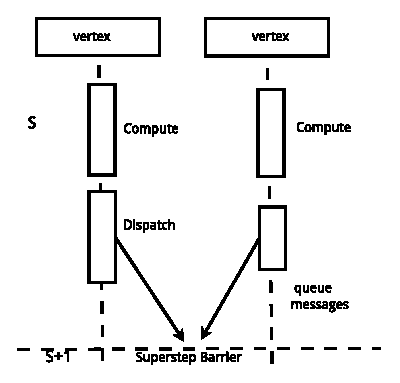
\includegraphics[width=\textwidth]{myfigures/sequentialbsp_new}
\caption{传统BSP模型}\label{fig:traBSP}
\end{minipage}
\begin{minipage}{0.4\textwidth}
\centering
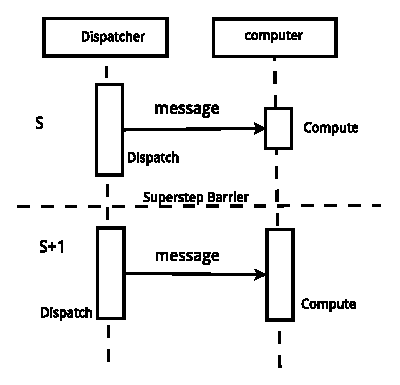
\includegraphics[width=\textwidth]{myfigures/computemodel}
\caption{改进后的BSP模型}\label{fig:newBSP}
\end{minipage}
\vspace{\baselineskip}
\end{figure}


\subsection{传统BSP模型的缺陷}
由于BSP模型的同步路障机制的存在,那么在整个BSP模型的垂直方向上,影响最终效率的关键就是最晚完成的任务,如图\ref{fig:bsp}所示。在基于传统BSP计算模型的图处理系统中,如图\ref{fig:traBSP}所示,图的处理主要分为两个阶段:以顶点为中心的计算(Compute)过程和消息的分发(Dispatch)过程。这两个过程按照严格的串行方式执行的,消息分发过程对计算过程存在数据依赖,形成强耦合。这种串行执行的方式,进一步延长了垂直方向上的任务完成的时间,降低的执行效率。在以顶点为中心的图计算中,消息时顶点之间的主要数据交换,顶点调用用户提供的计算函数对数据进行处理。消息包含计算所需的全部数据,所以相对于计算过程而言消息的具体分发过程是可以透明的。由于消息的生成和处理分布在两个相邻的超级步中,在该超级步结束之前,需要缓存大量的消息,并且在下一个超级步开始之前,这些消息不会被处理掉,增加额外的IO开销。
目前,基于BSP计算模型的图处理系统多任务并行处理的方法主要是采用多线程的技术。而线程是操作系统的基本调度单位,在操作系统中利用多线程在并发度上就会受到很大的限制。另外,由于需要保存大量的数据,当线程处理IO操作的时候,线程的调度会引发上下文的频繁切换,会对处理效率造成影响。

\subsection{Actor-BSP模型}

消息的分发过程和计算过程之间的主要依赖关系是消息,那么消息分发过程是消息的生产者,计算过程则是消息的消费者,两者之间以生产者和消费者的模式进行共存,从而将两者从严格串行的模式中解耦出来,如图\ref{fig:newBSP}所示。在改进后的BSP模型中,消息分发过程和计算过程位于两个单独的执行流程中。消息分发过程主要负责消息的生成和转发。计算过程侦听消息,当消息达到,计算过程则负责对消息进行处理及数据更新。
在语义上计算过程和消息分发过程是相互独立的轻量级调度单位。现有的BSP的实现在语义封装上往往是以顶点为中心,线程负责处理顶点。所以,在实现New BSP的模型中,采用轻量级、能够异步处理消息的并发模型成为关键。Actor并发模型相比于线程而言更加轻量级,有着更好的并发度。同时,Actor在语义上与Vertex的语义较为接近,兼顾了线程的调度执行和以顶点为中心的特点。



\section{数据组织}

单机的图处理系统同时具有计算密集型和IO密集型两个特点,合理的数据组织方式对整个系统的性能具有重要的影响。本节首先分析在Actor-BSP模型中数据的访问行为,然后根据数据的行为对GPSA的数据的组织方式进行说明和解释。

\subsection{数据访问行为}
在Actor-BSP模型中,Actor替换顶点成为整个计算展开的中心对象,之前顶点之间的消息的传递转变为Actor对象之间的消息通讯,从而导致新模型在数据读写方式上与传统的BSP模型不同。本小节从消息、顶点以及边的角度出发结合Actor-BSP模型展示其数据读写方式的行为特征。

首先,消息无需缓存。由于Actor-BSP模型中,由于生产者和消费者的组合,计算Actor监听消息到达事件,一旦事件到达消息就可以被及时处理。新模型无需为下一个超级步保存大量的消息,减少消息缓存的IO操作。

其次,只有分发Actor才会访问边。由于分发Actor主要任务就是生产消息,而消息的产生和发送都与边有着紧密的联系。但是,计算Actor不关心边的状态,只关心消息到达的事件以及如何处理消息与更新数据。

再次,顶点状态数据信息需要常驻内存来支持随机访问。在以顶点为中心的模型中,顶点是有状态信息的,当顶点开始对消息进行处理的时候,顶点自身的状态会包含在自己的数据域,并且参与到计算中。无状态的Actor不会持有特定消息所有者的顶点状态信息。如果计算Actor接收到消息,它需要获取消息所有者的状态信息,然后调用用户提供的函数对消息进行处理。然而无状态的Actor并不记录消息到来的顺序及消息所有者的任何信息,所以无状态的Actor在处理消息的时候需要能够随机获取消息所有者的状态信息。

最后,双份状态信息同时参与计算。在传统模型中,顶点的状态信息需要额外保存一份来判断状态是否发生更新。而在Actor-BSP模型中,顶点的状态信息的双份保存主要是因为分发Actor和计算Actor对状态信息读取的目的不同。分发Actor获取顶点的状态信息主要是产生消息,而计算Actor获取状态信息主要是用于处理消息,并且替换更新的状态信息。所以两者在获取的状态信息是不一致的。分发Actor获取的状态信息主要是来自初始化或者上一个超级步的结果,而计算Actor获取的状态信息却总是当前超步的最新结果。



\subsection{磁盘IO}
GraphChi和X-stream需要将大量的数据写入到磁盘中,因此对提高IO的性能有着非常高的要求。所以,Graphchi不遗余力的设计平行滑动窗口(PSW),并藉此实现异步的计算模型,并且为了实现PSW,GraphChi需要做非常多的预处理来满足要求。而X- stream也是从避免随机访问的角度出发采用顺序访问的Scatter和Gather两个阶段对图进行处理,同时采用异步IO的方式来获得更好的性能。

然而,在新的计算模型中,数据的访问方式发生较大的变化。不需要缓存消息意味着不需要为缓存大量的中间消息设计复杂的磁盘IO功能。边与顶点的分离,使得要处理的数据量减少很多。相比较整个庞大的图而言,顶点的状态信息就显得适合常驻内存进行处理来获取更好的性能。由于不需要向磁盘写入大量的数据,出于容错性的考虑,我们采用内存映射的方式对顶点的状态信息进行组织。而对于庞大数量的边而言,松散的组织结构可以省去一些耗时较长的预处理,同时满足顺序访问的特点,避免复杂的IO优化操作。

\subsection{数据组织设计}
图的数据主要分为两个部分,顶点的状态信息和边。其中,顶点的状态信息以二进制的格式存储在内存映射文件当中。边则以行压缩(Compressed Sparse Row)格式保存在磁盘上。

\begin{figure}[htbp]
\centering
\begin{minipage}{0.4\textwidth}
\centering
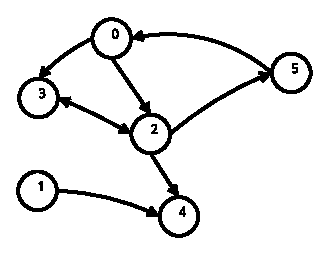
\includegraphics[width=\textwidth]{myfigures/graph.eps}
\caption{例图}\label{fig:graph}
\end{minipage}
\begin{minipage}{0.4\textwidth}
\centering
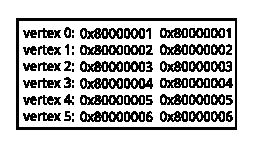
\includegraphics[width=0.8\textwidth]{myfigures/twocol.eps}
\caption{两列存储}\label{fig:twocol}
\end{minipage}
\begin{minipage}{0.4\textwidth}
\centering
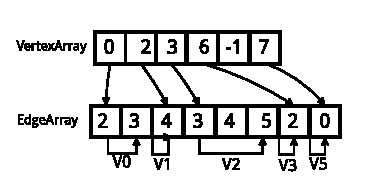
\includegraphics[width=\textwidth]{myfigures/csr.eps}
\caption{CSR存储}\label{fig:csr}
\end{minipage}
\begin{minipage}{0.4\textwidth}
\centering
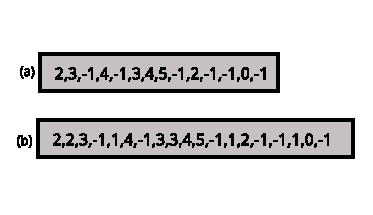
\includegraphics[width=\textwidth]{myfigures/ncsr.eps}
\caption{顺序存储}\label{fig:ncsr}
\end{minipage}

\vspace{\baselineskip}
\end{figure}

由于顶点的状态信息需要保存两份以供两种actor访问,所以在顶点状态信息的内存映射文件中,同一个顶点的状态信息以相邻的方式保存两份,就如同两排并列的数据,如图\ref{fig:twocol}所示。通过这种简单的方式,可以通过顶点\textit{id}计算顶点在整个文件中的偏移值来快速的获取顶点\textit{V}的状态信息的值,即$|V| * sizeof(Val)*2$。当该内存映射文件被映射到内存中后,整个访问的过程就像在操作一个数组一样方便。

CSR格式将顶点\textit{id}和边分别用两个数组进行保存,其中边数组保存边的目的顶点\textit{id}并按照出发顶点\textit{id}排序就,而在顶点数组中顶点的\textit{id}就是数组的索引,每个顶点保存第一条边在在边数组中的索引。此时,如果需要遍历第\textit{i}个顶点的边,那么只需要访问EdgeArray[VertexArray[i]],EdgeArray[VertexArray[i]+1],···,EdgeArray[VertexArray[i+1]]就可以完成该顶点边的遍历。如图\ref{fig:csr}所示,在遍历顶点\textit{Vertex 2}时,就可以通过访问[EdgeArray[3],EdgeArray[6])对边顶点进行遍历。CSR格式的空间效率是O(n+m),其中n和m分别是边和顶点的个数。另外,还可以在CSR格式的基础上采用顺序存储的方式,每个不同顶点的边之间用分割符加以分别,如图\ref{fig:ncsr}(a)所示,不同顶点之间可以用\textit{-1}作为分隔符,对边的遍历只需要读取到-1为止即可,除此之外还可以保存除边之外的其他信息,例如出度,权值等,在图\ref{fig:ncsr}(b)中就额外保存了每个顶点的出度,数组中第一个索引位置的值是2,表示此处顶点的的出度是2,紧接着的是两条边,当读取到-1的时候,顶点的\textit{id}递增加一。

\section{消息分发}
消息是本系统的重要关注和处理的对象,虽然Actor-BSP模型的优势使得无需为消息进行额外的缓存,但是合理的消息产生和分发策略对系统的效率有着重要的影响。
\subsection{消息}
一般来说消息的主要有两部分内容组成:目的顶点和消息的值。目的顶点表明该消息前往的顶点,同时也会影响由哪个具体的计算Actor来处理该消息。消息的值则是计算Actor用来进行计算的数据。虽然消息的生成工作主要是由分发Actor负责,但是消息的值的生成方法根据应用的不同具体的生成算法也不一样。例如,在遍历应用中,消息的值则是一个表示从源点开始到目前顶点的一个层次数,而在PageRank算法中,消息的值则是当前顶点的权值均分到他的出边邻接顶点的浮点数。所以,具体的消息的实现过程,由用户自己实现,分发Actor则调用具体的生成算法产生消息。
\subsection{分发策略}
当消息生成之后,分发Actor需要将消息分发给计算Actor。在Actor-BSP模型中,以顶点为中心的方式被无状态的Actor代替,计算Actor需要均衡的处理这些消息。虽然Actor的上下文切换远比线程轻量级,但是Actor的调度依然可能成为性能的制约因素,所以需要对消息的分发过程进行额外的硬性控制来避免某个计算Actor的负载过重。理论上来说,每个计算Actor都应该处理差不多个数的消息,但是由于图结构是无规律的,消息的发送目的地也有很大程度的随意性,在短时间内平均的将消息发送给计算Actor的可能性也微乎其微。为达到这样的目的,GPSA在预处理阶段对计算Actor进行了任务分配,将消息按照目的顶点的次序均分给计算Actor。在分发的过程中,如果某个计算Actor的邮箱已满,无法接受更多消息,那么该消息将会发送到目前消息数目最少的计算Actor的邮箱中,从而实现动态均衡。

\section{数据更新}
计算Actor接收到消息之后,调用用户实现的具体计算函数,如果经过计算之后顶点的状态发生改变,那么计算Actor就需要更新顶点的状态信息写入内存。由于计算Actor和分发Actor对数据访问的行为不同,所以需要两份不同的顶点信息的拷贝。其中一份拷贝供分发Actor查询使用,该数据是上一个超级步后的结果;另外一份拷贝则供计算Actor进行更新。由于两份数据以“Two-Column”的方式进行保存,两份数据就可以以列进行区分,如图\ref{fig:vu}所示。计算Actor和分发Actor对这两列数据依次交替访问,计算Actor访问的数据列是计算列,而分发Actor访问的数据列是分发列。

\begin{figure}[htbp]
\centering
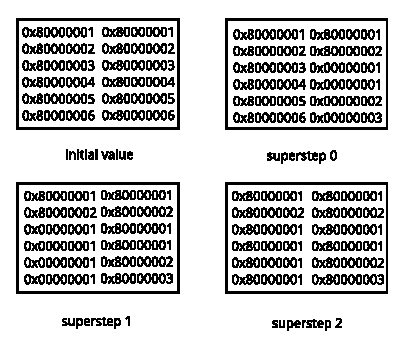
\includegraphics[width=0.4\textwidth]{myfigures/valueupdating.eps}
\caption{数据更新}\label{fig:vu}
\vspace{\baselineskip}
\end{figure}

在初始化结束之后,顶点的两列状态信息是相同的。分发Actor访问分发列的数据,然后计算Actor对计算列数据进行更新。在计算的过程中,为了避免消息的重复发送,同时保证计算Actor能够取得正确的顶点状态数据,将状态数据的最高位作为标识位。如果高位为1并且超级步\textit{i}大于0,则表示该数据在上一个超步中没有发生更新,分发Actor将会跳过该顶点,若高位为0,则说明数据在上一个超级步发生了更新,分发Actor会将此处数据对应的顶点的更新消息发送给它的邻接顶点,然后分发Actor将其高位置0。若超级步为0,则分发Actor会依次将顶点的状态信息发送出去。对于计算Actor,如果读取到的数据高位为1,则表明该数据尚未被更新,此时计算Actor将会读取该顶点的最新的状态信息,即从分发列对应位置获得最新值,如果计算之后顶点状态信息发生更新则把计算之后的新数据写入到当前顶点的计算列,否则不更新,下次读取数据依然从分发列读取数据。若计算Actor读取到的数据高位为0,则表明当前位置的数据是最新的,将会直接读取数据进行计算。如图\ref{fig:vu}所示,在初始化时,两列数据都相同并且最高位都为0。在超级步\textit{0}中,分发Actor对所有顶点的状态信息发送出去,计算Actor在接收到消息之后对计算列的数据进行更新。在超级步\textit{1}中,计算列和分发列互换位置,根据高位信息依次进行消息分发和数据更新。

\section{GPSA工作模块实现}
% 在上文,我们详细的分析了GPSA的设计细节,本部分则对GPSA的功能模块和实现过程进行详细的阐述。
% 在Actor-BSP模型的基础上,本文提出了基于新模型的单机图处理系统GPSA。通过实验证明,GPSA是一个具有高效、可扩展性与容错性的单机图处理系统。GPSA主要用JAVA编程语言实现,其中角色模型的实现采用了Kilim并发框架。本节将会对GPSA的组成和实现的过程进行详细的阐述。

GPSA的实现基于JAVA和Kilim角色并发框架。在GPSA中,输入是在上文中详述的以二进制形式保存的数据文件,包括顶点的状态信息和边的信息;输出则是经过计算之后图中顶点的状态信息。如图\ref{fig:overview},GPSA主要包括三个功能模块:预处理、Manager管理模块、Actor工作模块。预处理模块主要涉及对计算开始之前的初始化工作;Manager管理模块负责对计算进行协调与控制;分发Actor负责消息的产生和分发;计算Actor则是计算的基本执行单元。

·
\begin{figure}[htbp]
\centering
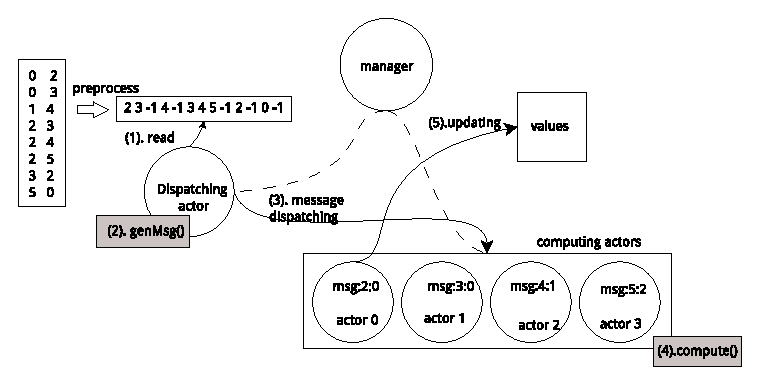
\includegraphics[width=0.8\textwidth]{myfigures/newexample.eps}
\caption{系统架构}\label{fig:overview}
\vspace{\baselineskip}
\end{figure}

\subsection{预处理}
GPSA默认对边集存储的数据进行预处理。
首先,边按照起始顶点的大小升序排序。虽然GPSA的新模型对分发过程和计算过程进行了分离,GPSA理论上只要能够获取边、起始顶点的顶点状态信息和用户自定义的消息生成的函数就可以发送消息并驱动计算Actor进行计算,也就是说GPSA可以处理原始的以边集存储的图。但是GPSA的新模型仍然是基于BSP模型的,耗费时间最长的任务将决定实际的计算效率,而直接对原始的边集数据进行计算,容易造成任务分配不均,计算效率低的结果。另外,在新模型中图的顶点信息是需要进行初始化并且映射到内存中的,需要与边区别对待。
在GPSA中,图是以CSR的格式进行存储的,需要将顶点和边分开,计算出图的一些基本信息,例如,边数、顶点数等,同时对任务进行分割。首先,预处理模块读取边,对边按照起始顶点的大小按升序的方式进行排序,如果起始顶点相同则按照目的顶点的大小升序排序。接下来,对排序之后的边进行CSR格式转换,将转换后的CSR格式的图数据写入磁盘,同时计算出图的基本信息,例如顶点的出度和入度、顶点个数,边的个数等等。

任务分割主要指计算任务的分割。对于消息分发Actor而言,顺序读取CSR数据即可;对于计算Actor而言,每个计算Actor所处理的消息个数应该相差不大,同时为避免有两个Actor同时操作同一顶点信息的更新而引起同步写,所以GPSA采用了一种“区间”的处理方法,即每个计算Actor负责连续的顶点闭区间$[i,j]$,每个区间接受的消息总数目接近每个计算Actor负责消息的平均值。

假设图的总边数为\textit{m},计算Actor个数为\textit{n},则每个计算Actor的区间处理的消息数目为\textit{k}满足以下条件:

\[\frac{m}{n} \le k < \frac{m}{{n - 1}}\]

预处理模块根据顶点的入度计算每个Actor所应处理的消息个数,并生成响应的区间对象,将其传递给Manager管理者。
\subsection{Manager管理模块}
Manager主要负责初始化计算,协调分发和计算的有序进行以及异常处理。在计算开始执行之前,图数据需要准备就绪,Manager调用预处理模块对图进行处理,根据图的基本信息计算出最小的顶点\textit{id}和最大的顶点\textit{id},调用用户定义初始化函数对顶点的状态信息进行初始化,并将结果写入顶点信息内存映射文件,完成对顶点初始信息的初始化。另外,manager需要根据用户指定的分发Actor和计算Actor数目,初始化对应数目的Actor。

初始化工作完成之后,Manager主要对计算过程进行协调。如算法\ref{algo:manager}所示,首先Manager向分发Actor发送\textit{ITERATION\_START}信号。接收到\textit{ITERATION\_START}信号的分发Actor会开始访问存储在磁盘上的CSR格式的图数据,调用用户定义的消息生成规则函数打包消息。当分发Actor在当前超级步的消息分发任务完成之后,分发Actor用\textit{DISPATCH\_OVER}信号通知Manager。如果所有的分发Actor都完成之后,Manager紧接着向所有的计算Actor发送\textit{COMPUTE\_OVER}信号。如果计算Actor处理到该消息则会意识到本超级步的计算工作已经完成,此时它会回复Manager一个同样的\textit{COMPUTE\_OVER}。最后,如果计算满足结束条件,Manager向所有的Actor发送\textit{SYSTEM\_OVER},当Actor接受到该信号将会退出自身的执行循环,结束生命周期。

\begin{algorithm}[htb!]
{
{

\renewcommand\baselinestretch{1.5}\selectfont %控制行距

\caption{Manager Execution Loop}
\label{algo:manager}
\begin{algorithmic}[1]
\REQUIRE ~\\
Initialize dispatchers,computers,mailbox, 

\STATE $counter \leftarrow 0$
\STATE $currIte \leftarrow 0$

\WHILE{ $currIte < endIte$ }
\FOR {$dispatcher \in dispatchers$}
\STATE $dispatcher \leftarrow ITERATION\_START$
\ENDFOR

\WHILE{ $(signal \leftarrow mailbox.get()) == DISPATCH\_OVER$}
\STATE $counter \leftarrow counter + 1$
\IF{$counter == dispatchers.length$}
\STATE $counter \leftarrow 0$
\STATE $break$
\ENDIF
\ENDWHILE

\FOR {$worker \in computers$}
\STATE $worker \leftarrow COMPUTE\_OVER$
\ENDFOR

\WHILE{ $(signal \leftarrow mailbox.get()) == COMPUTE\_OVER$}
\STATE $counter \leftarrow counter + 1$
\IF{$counter == computers.length$}
\STATE $counter \leftarrow 0$
\STATE $break$
\ENDIF
\ENDWHILE

\STATE $currIte \leftarrow currIte + 1$
\ENDWHILE
\end{algorithmic}
}
\par}
\end{algorithm}

\subsection{Actor工作模块}
Actor模块系统中最重要的组成部分,该模块主要负责消息的生成和计算并更新数据。在该模块中主要包含两种无状态Actor:分发Actor和计算Actor。

%分发Actor从磁盘上顺序读取边,根据初始化信息或者上个超级步中顶点的更新情况,调用用户自定义的消息产生函数生成新消息,并将消息发送到边的目的顶点所对应的计算Actor。
分发Actor的工作流程如算法\ref{algo:dispatcher} 所示,分发Actor等待来自Manager的\textit{ITERATION\_START}的信号,接收到信号后分发Actor开始进入执行循环,检查处理的边的起止信息,从起止信息的起始位置开始顺序从磁盘上读取一条边,获取该边起始顶点的顶点的状态信息,如果当前超级步不是0并且信息高位为1,则表明当前顶点的状态信息在上一个超级步中没有发生更新,需要跳过该顶点,继续处理下一个顶点,\textit{skip(sequence)}函数,则会让当前的的顶点\textit{id}加1,同时跳过该顶点的所有边,寻址到下一个顶点的第一条边的偏移地址。若当前超级步为0或者高位为0,则表明该顶点处于初始化之后的状态或者在上一个超级步中发生了更新,分发Actor调用用户提供的\textit{genMsg()}实现生成消息,根据分发策略将消息发送出去。如果读取边的目的顶点为-1,则表明当前顶点处理完毕,并将该顶点的状态信息状态最高位置1表明处理完成。如此周而复始,直至完成分发任务,分发Actor用\textit{DISPATCH\_OVER}通知Manager。

\begin{algorithm}
{
{

\renewcommand\baselinestretch{1.5}\selectfont %控制行距

\caption{Dispatcher Execution Loop}
\label{algo:dispatcher}
\begin{algorithmic}[1]

\STATE
 $signal \leftarrow mailbox.get()$
\WHILE{ $signal != SYSTEM\_OVER$ }
\IF{$interval != null$}
\STATE $ reset() $
\WHILE{$curoff < endoff$}
\STATE $val \leftarrow getValue(sequence)$

\IF{$isHighestBit(val)==1 \&\& currIte != 0$}
\STATE $skip(sequence)$
\ENDIF

\IF{$isHighestBit(val)==0 \|\| currIte == 0$}
\STATE $vid \leftarrow readEdge(curoff)$
\WHILE{$curoff < enfoff $}
\IF{$vid == -1$}
\STATE $break$
\ENDIF
\STATE $msg \leftarrow genMsg()$
\STATE $DispatchStrategy(vid,msg)$
\ENDWHILE
\STATE $setHighesetBitTo1()$
\ENDIF
\ENDWHILE
\ENDIF
\STATE $notifyManager(DISPATCH\_OVER)$
\STATE $signal \leftarrow mailbox.get()$
\ENDWHILE

\end{algorithmic}
}
\par}
\end{algorithm}


计算Actor的工作流程如算法\ref{algo:computer}所示,计算Actor等待来自Manager的消息,然后进入执行循环体。否则计算Actor从消息中提取目的顶点和消息的值,根据目的顶点从顶点的状态信息内存映射文件中读取顶点值,然后调用用户提供的\textit{compute(val,msgVal)}实现对其进行计算,计算返回一个新的顶点状态信息。如果新的顶点状态与之前的值相比发生了改变,则将新数据更新到内存映射文件,否则丢弃。如此迭代,直到计算Actor接受到的信号是\textit{COMPUTE\_OVER},则表示当前的超级步的计算完成,同时用\textit{COMPUTE\_OVER}回复Manager。如果计算Actor接收到\textit{SYSTEM\_OVER}信号,则会结束计算退出循环。

\begin{algorithm}
{
{
\renewcommand\baselinestretch{1.5}\selectfont %控制行距

\caption{Compute Execution Loop}
\label{algo:computer}
\begin{algorithmic}[1]

\STATE $msg \leftarrow mailbox.get()$
\WHILE{ $signal != SYSTEM\_OVER$ }
\IF{$msg == COMPUTE\_OVER$}
\STATE $notifyManager(COMPUTE\_OVER)$
\ELSE
\STATE $to \leftarrow msg.dest()$
\STATE $msgVal \leftarrow msg.val()$
\STATE $val \leftarrow getVal(to)$
\STATE $newVal \leftarrow compute(val,msgVal)$
\IF{$newVal != val$}
	\STATE $update()$
\ENDIF
\ENDIF
\STATE $msg \leftarrow mailbox.get()$
\ENDWHILE


\end{algorithmic}
}
\par}
\end{algorithm}


\section{小结}

本章首先介绍常见的用于图计算的模型,并讨论了BSP模型中的缺陷。接下来在传统BSP模型的基础上,使用Actor将计算过程和分发过程分开。然后围绕Actor-BSP模型中的数据行为、磁盘IO、消息分发和数据更新等内容对GPSA系统进行设计和规划。最后,在此基础上,本章对GPSA的系统实现进行阐述和说明。从功能模块上划分,GPSA主要分为预处理模块、Manger管理模块、计算Actor和分发Actor模块。预处理模块对数据进行数据格式的转换与信息分离,以及任务分配等工作。Manager则是系统的执行计算的控制单元,负责协调计算Actor和分发Actor的开始和进行,以及一些异常处理。计算Actor和分发Actor模块则是主要的运算模块,其中分发Actor从磁盘读取一条边,根据用户的消息生成规则产生消息,并将消息分发给计算Actor,而计算Actor在接受到消息之后,会根据消息访问顶点信息,调用用户的\textit{compute(val,msgVal)}函数进行计算并取得返回值,然后判定是否发生更新,并将更新数据写入内存。

% !Mode:: "TeX:UTF-8"

\chapter{基于Actor-BSP模型的单机多核系统的图计算}

\section{Actor-BSP模型}

\section{图计算框架}
\subsection{..}
\subsection{..}
\subsection{..}
\subsection{..}







% !Mode:: "TeX:UTF-8"

\chapter{模板介绍与注意事项}
\section{模板说明}

HNUThesis~是为了帮助湖南大学毕业生撰写毕业论文而编写的~\LaTeX~论文模板,其前提是用户已经能处理一般的~\LaTeX~文档,并对~BibTeX~有一定了解,如果你从来没有接触过~\LaTeX~,建议先学习相关基础知识,磨刀不误砍柴工,能有助你更好使用模板。

由于个人水平有限,虽然现在的这个版本基本上满足了学校的要求,但难免存在不足之处,欢迎大家积极反馈,更希望湖南大学~\LaTeX~爱好者能一同完善此模板,让更多同学受益。

如有模板的疑问或有意向加入模板的维护和编写队伍中来,请给作者: maxdujiayi@gmail.com(杜家宜)写信。

\section{下载安装}
HNUThesis~主页:~\url{http://hnuthesis.googlecode.com/}。除此之外,不再维护任何镜像。

\section{目录内容}
本~\LaTeX{}~模板的源文件即为研究生毕业设计论文中使用的模板,用户可以通过修改这些文件来编辑自己的毕业论文。
\begin{itemize}
\item{hnumain.tex}:主文件,包含封面部分和其他章节的引用信息。
\item{preface}: 包含本科毕业设计论文的封面和中英文摘要。
\item{body}: 包含本文正文中的所有章节。
\begin{itemize}
\item{intros.tex}: 包括本~\LaTeX{}~模板的介绍,编译方法和使用方法。
\item{figures.tex}: 包含论文中图片的插入和引用方法。
\item{tables.tex}: 包含论文中表格的插入和引用方法。
\item{equations.tex}: 包含论文中数学符号、公式的书写和排版方法。
\item{others.tex}: 包含论文中使用的罗列环境,定理环境等其他环境的排版方法。
\item{conclusion.tex}: 包含本文的总结。
\end{itemize}
\item{setup}:存放论文所使用的宏包和全文格式的定义。
\item{appendix}:存放作者的发表论文和参加科研情况说明以及致谢文件。
\item{references/reference.bib}:存放论文所引用的全部参考文献信息。
\item{clean.bat}:双击此文件,可以用来清理~hnumain.tex~在编译之后生成的所有附属文件,如后缀名为~.aux~,~.log~,~.bak~的文件。
\end{itemize}

需要说明的是,以上文件名并不是固定的,各位同学可以新建一个~tex~文件,例如~algorithm.tex,放在~body~目录下,并且在~hnumain.tex~中调用:
\begin{verbatim}
    \include{body/algorithm.tex}
\end{verbatim}
来引用之。当然你也可以重命名这些文件,只要~include~中的文件名是存在且合法,~\LaTeX~总能找到这些文件的。

在你写作某一章节的时候,你可能需要随时预览排版效果并~Debug,这时你可以在其他章节的\verb|\include|命令前加上一个\%,这代表注释掉本行,例如:
\begin{verbatim}
%%%%%%%%%%%%%%%%%%%%%%%%%%%%%%%%
           正文部分
%%%%%%%%%%%%%%%%%%%%%%%%%%%%%%%%
\mainmatter
% !Mode:: "TeX:UTF-8"

\chapter{模板介绍与注意事项}
\section{模板说明}

HNUThesis~是为了帮助湖南大学毕业生撰写毕业论文而编写的~\LaTeX~论文模板,其前提是用户已经能处理一般的~\LaTeX~文档,并对~BibTeX~有一定了解,如果你从来没有接触过~\LaTeX~,建议先学习相关基础知识,磨刀不误砍柴工,能有助你更好使用模板。

由于个人水平有限,虽然现在的这个版本基本上满足了学校的要求,但难免存在不足之处,欢迎大家积极反馈,更希望湖南大学~\LaTeX~爱好者能一同完善此模板,让更多同学受益。

如有模板的疑问或有意向加入模板的维护和编写队伍中来,请给作者: maxdujiayi@gmail.com(杜家宜)写信。

\section{下载安装}
HNUThesis~主页:~\url{http://hnuthesis.googlecode.com/}。除此之外,不再维护任何镜像。

\section{目录内容}
本~\LaTeX{}~模板的源文件即为研究生毕业设计论文中使用的模板,用户可以通过修改这些文件来编辑自己的毕业论文。
\begin{itemize}
\item{hnumain.tex}:主文件,包含封面部分和其他章节的引用信息。
\item{preface}: 包含本科毕业设计论文的封面和中英文摘要。
\item{body}: 包含本文正文中的所有章节。
\begin{itemize}
\item{intros.tex}: 包括本~\LaTeX{}~模板的介绍,编译方法和使用方法。
\item{figures.tex}: 包含论文中图片的插入和引用方法。
\item{tables.tex}: 包含论文中表格的插入和引用方法。
\item{equations.tex}: 包含论文中数学符号、公式的书写和排版方法。
\item{others.tex}: 包含论文中使用的罗列环境,定理环境等其他环境的排版方法。
\item{conclusion.tex}: 包含本文的总结。
\end{itemize}
\item{setup}:存放论文所使用的宏包和全文格式的定义。
\item{appendix}:存放作者的发表论文和参加科研情况说明以及致谢文件。
\item{references/reference.bib}:存放论文所引用的全部参考文献信息。
\item{clean.bat}:双击此文件,可以用来清理~hnumain.tex~在编译之后生成的所有附属文件,如后缀名为~.aux~,~.log~,~.bak~的文件。
\end{itemize}

需要说明的是,以上文件名并不是固定的,各位同学可以新建一个~tex~文件,例如~algorithm.tex,放在~body~目录下,并且在~hnumain.tex~中调用:
\begin{verbatim}
    \include{body/algorithm.tex}
\end{verbatim}
来引用之。当然你也可以重命名这些文件,只要~include~中的文件名是存在且合法,~\LaTeX~总能找到这些文件的。

在你写作某一章节的时候,你可能需要随时预览排版效果并~Debug,这时你可以在其他章节的\verb|\include|命令前加上一个\%,这代表注释掉本行,例如:
\begin{verbatim}
%%%%%%%%%%%%%%%%%%%%%%%%%%%%%%%%
           正文部分
%%%%%%%%%%%%%%%%%%%%%%%%%%%%%%%%
\mainmatter
% !Mode:: "TeX:UTF-8"

\chapter{模板介绍与注意事项}
\section{模板说明}

HNUThesis~是为了帮助湖南大学毕业生撰写毕业论文而编写的~\LaTeX~论文模板,其前提是用户已经能处理一般的~\LaTeX~文档,并对~BibTeX~有一定了解,如果你从来没有接触过~\LaTeX~,建议先学习相关基础知识,磨刀不误砍柴工,能有助你更好使用模板。

由于个人水平有限,虽然现在的这个版本基本上满足了学校的要求,但难免存在不足之处,欢迎大家积极反馈,更希望湖南大学~\LaTeX~爱好者能一同完善此模板,让更多同学受益。

如有模板的疑问或有意向加入模板的维护和编写队伍中来,请给作者: maxdujiayi@gmail.com(杜家宜)写信。

\section{下载安装}
HNUThesis~主页:~\url{http://hnuthesis.googlecode.com/}。除此之外,不再维护任何镜像。

\section{目录内容}
本~\LaTeX{}~模板的源文件即为研究生毕业设计论文中使用的模板,用户可以通过修改这些文件来编辑自己的毕业论文。
\begin{itemize}
\item{hnumain.tex}:主文件,包含封面部分和其他章节的引用信息。
\item{preface}: 包含本科毕业设计论文的封面和中英文摘要。
\item{body}: 包含本文正文中的所有章节。
\begin{itemize}
\item{intros.tex}: 包括本~\LaTeX{}~模板的介绍,编译方法和使用方法。
\item{figures.tex}: 包含论文中图片的插入和引用方法。
\item{tables.tex}: 包含论文中表格的插入和引用方法。
\item{equations.tex}: 包含论文中数学符号、公式的书写和排版方法。
\item{others.tex}: 包含论文中使用的罗列环境,定理环境等其他环境的排版方法。
\item{conclusion.tex}: 包含本文的总结。
\end{itemize}
\item{setup}:存放论文所使用的宏包和全文格式的定义。
\item{appendix}:存放作者的发表论文和参加科研情况说明以及致谢文件。
\item{references/reference.bib}:存放论文所引用的全部参考文献信息。
\item{clean.bat}:双击此文件,可以用来清理~hnumain.tex~在编译之后生成的所有附属文件,如后缀名为~.aux~,~.log~,~.bak~的文件。
\end{itemize}

需要说明的是,以上文件名并不是固定的,各位同学可以新建一个~tex~文件,例如~algorithm.tex,放在~body~目录下,并且在~hnumain.tex~中调用:
\begin{verbatim}
    \include{body/algorithm.tex}
\end{verbatim}
来引用之。当然你也可以重命名这些文件,只要~include~中的文件名是存在且合法,~\LaTeX~总能找到这些文件的。

在你写作某一章节的时候,你可能需要随时预览排版效果并~Debug,这时你可以在其他章节的\verb|\include|命令前加上一个\%,这代表注释掉本行,例如:
\begin{verbatim}
%%%%%%%%%%%%%%%%%%%%%%%%%%%%%%%%
           正文部分
%%%%%%%%%%%%%%%%%%%%%%%%%%%%%%%%
\mainmatter
\include{body/intros}
%%\include{body/figures}
%%\include{body/tables}
%%\include{body/equations}
%%\include{body/others}
%%\include{body/conclusion}
\end{verbatim}
那么,编译的时候就只编译未加~\%~的一章,在这个例子中,即本章~intros。

理论上,并不一定要把每章放在不同的文件中。但是这种自顶向下,分章节写作、编译的方法有利于提高效率,大大减少~Debug~过程中的编译时间,同时减小风险。

\section{参考文献生成方法}

\LaTeX~具有插入参考文献的能力。Google Scholar~网站上存在兼容~BibTeX~的参考文献信息,通过以下几个步骤,可以轻松完成参考文献的生成。
\begin{itemize}
  \item 在\href{http://scholar.google.com/}{谷歌学术搜索}中,
        点击\href{http://scholar.google.com/scholar_preferences?hl=en&as_sdt=0,5}{学术搜索设置}。
  \item 页面打开之后,在\textbf{文献管理软件}选项中选择\textbf{显示导入~BibTeX~的链接},单击保存设置,退出。
  \item 在谷歌学术搜索中检索到文献后,在文献条目区域单击导入~BibTeX~选项,页面中出现文献的引用信息。
  \item 将文献引用信息的内容复制之后,添加到~references~文件夹下的~reference.bib~中。
\end{itemize}

\section{编译注意事项}
\begin{enumerate}
  \item 由于模板使用~UTF-8~编码,所以源文件应该保存成~UTF-8~格式,否则可能出现中文字符无法识别的错误。
  本模板中每一个~.tex~文件的文件的开头已经加上一行:\\
    \verb|% !Mode:: "TeX:UTF-8"|\\
     这样可以确保~.tex~文件默认使用~UTF-8~的格式打开。读者如果删去此行,很有可能会导致中文字符显示乱码。
     在~WinEdt~编辑器中可以使用以下两种方式保存成~UTF-8~格式:
      \begin{enumerate}
        \item 先建立~.tex~文件,另存为~.tex~文件时,选择用~UTF-8~格式保存。
        \item
            在~WinEdt~编辑器中,选择\\
            \mbox{~Document$\to$Document Settings$\to$Document Mode $\to$TeX:UTF-8} 同时在~WinEdt~最下面的状态栏中,可以看到该文档是~TeX~格式还是~TeX:UTF-8~格式。
            当文档为~TeX:UTF-8~格式时,状态栏一般显示:
            \makebox[\textwidth][l]{Wrap | Indent | INS | LINE |Spell | TeX:UTF-8 | -src~等。}
      \end{enumerate}
  \item 如果在pdf书签中,中文显示乱码的话,则注意以下说明:
    \begin{verbatim}
        \usepackage{CJKutf8}
        % 1. 如果使用CJKutf8
        %    Hyperref中应使用unicode参数
        % 2. 如果使用CJK
        %    Hyperref则使用CJKbookmarks参数
        %    可惜得到的PDF书签是乱码,建议弃用
        % 3. Unicode选项和CJKbookmarks不能同时使用
        \usepackage[
        %CJKbookmarks=true,
        unicode=true
        ]{hyperref}
     \end{verbatim}
 \item 建议采用以下两种编译方式:
  \begin{enumerate}
     \item latex + bibtex + latex + latex + dvi2pdf. 在这种编译情况下,对应的~hnumain.tex~文件的第一行是\verb|\def\usewhat{dvipdfmx}|~(缺省设置)。 此时,所有图片文件应该保存为~.eps~格式,如~figures~文件夹里~.eps~图片。
          如果您选择在命令行中操作,可以在编译的时候依次输入~latex hnumain, bibtex hnumain, latex hnumain, latex hnumain~和~dvipdfmx hnumain, 编译完成之后,需要手动打开~pdf~文件。
     \item pdflatex + pdflatex. 在这种编译情况下,对应的~hnumain.tex~文件的第一行应该改为\verb|\def\usewhat{pdflatex}|~。 此时, 编译不支持~.eps~图片格式,此时需要在命令行下使用~epstopdf~指令将~figures~文件夹下 的~.eps~文件转化成~.pdf~文件格式,命令行中操作格式为~epstopdf a.eps~。
          在命令行编译的时候,依次输入~pdflatex hnumain~和~pdflatex hnumain, 编译完成之后,需要手动打开~pdf~文件。
  \end{enumerate}
\end{enumerate}

\section{系统要求}
    CTEX 2.8, MiKTeX 2.8, TeX Live 2009~或以上版本。使用推荐的~WinEdt 6.0~编辑器,可以完成文件的编辑和编译工作。

\section{\TeX~简介}

以下内容是~milksea@bbs.ctex.org~撰写的关于~\TeX~的简单介绍,略有改动。
注意这不是一个入门教程,不讲~\TeX~系统的配置安装,也不讲具体的~\LaTeX~代码。
这里仅仅试图以一些只言片语来解释:
进入这个门槛之前新手应该知道的注意事项,以及遇到问题以后该去如何解决问题。

\subsection{什么是 \TeX/\LaTeX,我是否应该选择它~?}

\TeX~是最早由高德纳(Donald Knuth)教授创建的一门标记式宏语言,
用来排版科技文章,尤其擅长处理复杂的数学公式。\TeX~同时也是处理这一语言的排版软件。
\LaTeX~是 Leslie Lamport 在~\TeX~基础上按内容/格式分离和模块化等思想建立的一集~\TeX~上的格式。

\TeX~本身的领域是专业排版领域
但现在~TeX/LaTeX~也被广泛用于生成电子文档甚至幻灯片等,~\TeX~语言的数学部分
偶尔也在其他一些地方使用。但注意~\TeX~并不适用于文书处理(Microsoft Office 的领域,以前和现在都不是)。

选择使用~\TeX/\LaTeX~的理由包括:
\begin{itemize}
\item 免费软件;
\item 专业的排版效果;
\item 是事实上的专业数学排版标准;
\item 广泛的西文期刊接收甚或只接收 LaTeX 格式的投稿;
\item[] ……
\end{itemize}
不选择使用~\TeX/\LaTeX~的理由包括:
\begin{itemize}
\item 需要相当精力学习;
\item 图文混合排版能力不够强;
\item 仅在数学、物理、计算机等领域流行;
\item 中文期刊的支持较差;
\item[] ……
\end{itemize}

请尽量清醒看待网上经常见到的关于~\TeX~与其他软件的优劣比较和口水战。在选择使用或离开之前,请先考虑
\TeX~的应用领域,想想它是否适合你的需要。


\subsection{我该用什么编辑器~?}

编辑器功能有简有繁,特色不一,从简单的纯文本编辑器到繁复的 Emacs,因人而易。基本功能有语法高亮、方便编译预览就很好了,扩充功能和定制有无限的可能。初学者可以使用功能简单、使用方便的专用编辑器,如 ~TeXWorks、Kile、WinEdt~等,或者类似所见即所得功能的~LyX;熟悉的人可以使用定制性更强的~Notepad++、SciTE、Vim、Emacs ~等。这方面的介绍很多,一开始不妨多试几种,找到最适合自己的才是最好的。

另外提醒一句,编辑器只是工作的助手,不必把它看得太重。

\subsection{我应该看什么~\LaTeX~读物~?}

这不是一个容易回答的问题,因为有许多选择,也同样有许多不合适的选择。
这里只是选出一个比较好的答案。更多更详细的介绍可以在版面和网上寻找(注意时效)。

近两年~\TeX~的中文处理发展很快,目前没有哪本书在中文处理方面给出一个最新进展的合适综述,
因而下面的介绍也不主要考虑中文处理。

\begin{enumerate}

\item 我能阅读英文。
\begin{enumerate}
\item 迅速入门:ltxprimer.pdf (LaTeX Tutorials: A Primer, India TUG)
\item 系统学习:A Guide to LaTeX, 4th Edition, Addison-Wesley
               有机械工业出版社的影印版(《\LaTeX{}~实用教程》)
\item 深入学习:要读许多书和文档,TeXbook 是必读的
\item 细节学习:去读你使用的每一个宏包的说明文档
\item 专题学习:阅读讲数学公式、图形、表格、字体等的专题文档
\end{enumerate}

\item 我更愿意阅读中文。
\begin{enumerate}
\item 迅速入门:lnotes.pdf (LaTeX Notes, 1.20, Alpha Huang)
\item 系统学习:《\LaTeXe{}~科技排版指南》,邓建松(电子版)
      如果不好找,可以阅读《\LaTeXe~入门与提高》第二版,陈志杰等,或者 《\LaTeXe~完全学习手册》,胡伟
\item 深入学习:~TeXbook0.pdf~(特可爱原本,TeXbook 的中译,xianxian)
\item 具体问题释疑:~CTeX-FAQ.pdf~,\\
        吴凌云,~\url{http://www.ctex.org/CTeXFAQ}~
\end{enumerate}
\end{enumerate}

遇见问题和解决问题的过程可以快速提高自己的技能,建议此时:
\begin{itemize}
  \item 利用~Google~搜索。
  \item 清楚,扼要地提出你的问题。
\end{itemize}

\subsection{什么知识会过时~?什么不会~?}

\TeX~是排版语言,也是广泛使用的软件,并且不断在发展中;
因此,总有一些东西会很快过时。作为学习~\TeX~的人,
免不了要看各种各样的书籍、电子文档和网络论坛上的只言片语,
因此了解什么知识会迅速过时,什么知识不会是十分重要的。

最稳定的是关于~Primitive \TeX~和~Plain \TeX~的知识,也就是 Knuth
在他的《The TeXbook》中介绍的内容。因为~\TeX~
系统开发的初衷就是稳定性,要求今天的文档到很久以后仍可以得到完全相同的结果,
因此 Knuth 限定了他的~\TeX~语言和相关实现的命令、语法。这些内容许多年来就没有多少变化,
在未来的一些年里也不会有什么变化。
Primitive \TeX~和 Plain \TeX~的知识主要包括 \TeX~排版的基本算法和原理,
盒子的原理,底层的 \TeX~命令等。其中技巧性的东西大多在宏包设计中,
初学者一般不会接触到很多;而基本原理则是常常被提到的,
譬如,~\TeX~把一切排版内容作为盒子(box)处理。

相对稳定的是关于基本~\LaTeXe~
的知识,也包括围绕~\LaTeXe~的一些核心宏包的知识。~\LaTeXe~
是自~1993~年以来的一个稳定的~\LaTeX~版本,直到最近的一次修订
(2005 年)都没有大的变动。
\LaTeX~的下一个计划中的版本~\LaTeX 3~遥遥无期,在可预见的将来,~\LaTeXe~不会过时。
\LaTeXe~的知识是目前大部分~\LaTeX~书籍的主体内容。关于~\LaTeX~的标准文档类
~(article、report、book、letter、slide~等),关于基本数学公式的输入,
文档的章节层次,表格和矩阵,图表浮动体,LR 盒子与段落盒子……
这些~\LaTeX~的核心内容都是最常用的,相对稳定的。
与~\LaTeXe~相匹配的核心宏包,
如~graphics(x)、ifthen、fontenc、doc~等,也同样是相对稳定的。
还有一些被非常广泛应用的宏包,如~amsmath~系列,也可以看作是相对稳定的。

简单地说,关于基本~\TeX/\LaTeX~的语言,都是比较稳定的。与之对应,实现或者支持~\TeX/\LaTeX~语言的软件,
包括在~\TeX/\LaTeX~基础上建立的新的宏,都不大稳定。

容易过时的是关于第三方~\LaTeX~宏包的知识、第三方~\TeX~工具的知识,以及新兴~\TeX~相关软件的知识等。
~\TeX~和~\LaTeX~语言是追求稳定的;但无论是宏包还是工具,作为不断更新软件,它们是不稳定的。
容易过时的技术很多,而且现在广泛地出现在几乎所有~\LaTeX~文档之中,因此需要特别引起注意:
宏包的过时的原因可
网络论坛上的只言片语的因此了解什么知识会迅速过时的什么知识不会是十分重
网络论坛上的只言片语的因此了解什么知识会迅速过时的什么知识不会是十分重
网络论坛上的只言片语的因此了解什么知识会迅速过时的什么知识不会是十分重
网络论坛上的只言片语的因此了解什么知识会迅速过时的什么知识不会是十分重
网络论坛上的只言片语的因此了解什么知识会迅速过时的什么知识不会是十分重
网络论坛上的只言片语的因此了解什么知识会迅速过时的什么知识不会是十分重
网络论坛上的只言片语的因此了解什么知识会迅速过时的什么知识不会是十分重
网络论坛上的只言片语的因此了解什么知识会迅速过时的什么知识不会是十分重
网络论坛上的只言片语的因此了解什么知识会迅速过时的什么知识不会是十分重
网络论坛上的只言片语的因此了解什么知识会迅速过时的什么知识不会是十分重
网络论坛上的只言片语的因此了解什么知识会迅速过时的什么知识不会是十分重
网络论坛上的只言片语的因此了解什么知识会迅速过时的什么知识不会是十分重
网络论坛上的只言片语的因此了解什么知识会迅速过时的什么知识不会是十分重
网络论坛上的只言片语的因此了解什么知识会迅速过时的什么知识不会是十分重
网络论坛上的只言片语的因此了解什么知识会迅速过时的什么知识不会是十分重
网络论坛上的只言片语的因此了解什么知识会迅速过时的什么知识不会是十分重
网络论坛上的只言片语的因此了解什么知识会迅速过时的什么知识不会是十分重
网络论坛上的只言片语的因此了解什么知识会迅速过时的什么知识不会是十分重
网络论坛上的只言片语的因此了解什么知识会迅速过时的什么知识不会是十分重
网络论坛上的只言片语的因此了解什么知识会迅速过时的什么知识不会是十分重
网络论坛上的只言片语的因此了解什么知识会迅速过时的什么知识不会是十分重
网络论坛上的只言片语的因此了解什么知识会迅速过时的什么知识不会是十分重
网络论坛上的只言片语的因此了解什么知识会迅速过时的什么知识不会是十分重
网络论坛上的只言片语的因此了解什么知识会迅速过时的什么知识不会是十分重
网络论坛上的只言片语的因此了解什么知识会迅速过时的什么知识不会是十分重
网络论坛上的只言片语的因此了解什么知识会迅速过时的什么知识不会是十分重
网络论坛上的只言片语的因此了解什么知识会迅速过时的什么知识不会是十分重
网络论坛上的只言片语的因此了解什么知识会迅速过时的什么知识不会是十分重
网络论坛上的只言片语的因此了解什么知识会迅速过时的什么知识不会是十分重
网络论坛上的只言片语的因此了解什么知识会迅速过时的什么知识不会是十分重
网络论坛上的只言片语的因此了解什么知识会迅速过时的什么知识不会是十分重
网络论坛上的只言片语的因此了解什么知识会迅速过时的什么知识不会是十分重
网络论坛上的只言片语的因此了解什么知识会迅速过时的什么知识不会是十分重
网络论坛上的只言片语的因此了解什么知识会迅速过时的什么知识不会是十分重
网络论坛上的只言片语的因此了解什么知识会迅速过时的什么知识不会是十分重
网络论坛上的只言片语的因此了解什么知识会迅速过时的什么知识不会是十分重
网络论坛上的只言片语的因此了解什么知识会迅速过时的什么知识不会是十分重
能是宏包本身的升级换代带来了新功能或不兼容,
也可能是同一功能的更新更好的宏包代替了旧的宏包。前者的典型例子比如绘图宏包~PGF/TikZ~,
现在的~2.00~版功能十分强大,和旧的~1.1x~版相差很大,和更旧的~0.x~版本则几乎完全不同;后
者的典型例子比如~caption~宏包先是被更新的~caption2~宏包代替,后来~caption~宏包更新又使得
caption2 宏包完全过时。——安装更新的发行版可以避免使用过旧的宏包;
认真阅读宏包自带的文档而不是搜索得到的陈旧片断可以避免采用过时的代码。

工具过时的主要原因也是升级换代和被其他工具替换。前者的典型例子是编辑器
WinEdt~在~5.5~以后的版本支持~UTF-8~编码,而旧版本不支持;
后者的典型例子是中文字体安装工具从~GBKFonts~到~xGBKFonts~到~FontsGen~不断被取代。
图形插入是一个在~\TeX~实现、宏包与外围工具方面都更新很快的东西。
在过去,最常用的输出格式是~PS(PostScript)~格式,因此插入的图像以~EPS~为主流。
使用~Dvips~为主要输出工具,外围工具有~GhostScript、bmeps~等等,相关宏包有~graphics~等,
相关文档如《\LaTeXe{}~ 插图指南》。

但凡提及“~\LaTeX~只支持~EPS~图形”的,就是这个过时的时代的产物。事实上~\TeX/\LaTeX~
并不限定任何图形格式,只不过是当时的输出格式(PS)和工具(Dvips)对~EPS~情有独钟而已。
后来 PDF 格式成为主流。~pdf\TeX、DVIPDFM、DVIPDFMx、XeTeX~工具则主要支持~PDF、PNG、JPG~格式的图形,
涉及一系列工具如~ImageMagick、ebb~等。

值得特别提出注意的就是,中文处理也一起是更新迅速、容易过时的部分。
而且因为中文处理一直没有一个“官方”的“标准”做法,软件、工具、
文档以及网上纷繁的笔记也就显得相当混乱。从八十年代开始的~CCT~系统、
天元系统,到后来的~CJK~方式,到近来的~XeTeX~和~LuaTeX~ 方式,
中文处理的原理、软件、宏包、配置方式等都在不断变化中。

%\section{后期工作}
%下表记录了~HNUThesis~计划中未来应该逐步实现的功能和特性:
%\begin{enumerate}
%  \item 编写更为详细的~HNUThesis~的使用手册和~FAQ~用户指南
%  \item 加入对课程结课论文的支持
%  \item 加入对天津大学学生经常参加的各种限时完成重大赛事的论文模板的支持,如全国研究生数学建模竞赛,以节省排版时间
%  \item 加入对~pdf~书签中章节中文编号的支持,如: 第1章 XXX
%  \item 加入对附录~A~等格式的支持
%  \item Linux~平台迁移和测试
%\end{enumerate}

\section{免责声明}

本模板依据《湖南大学关于博士、硕士学位论文统一格式的规定》和《湖南大学硕士论文模版》编写,适用于所有博士生的学位论文编写。然而,作者不保证本模板完全符合学校要求,也不对由此带来的风险和损失承担任何责任。

%%% !Mode:: "TeX:UTF-8"

\chapter{图片的插入方法}

\section{研究生毕业论文的插图规范}

图应有自明性。插图应与文字紧密配合,文图相符,内容正确。选图要力求精练,插图、照片应完整清晰。图中文字和数字等字号用宋体五号字。

机械工程图:采用第一角投影法,严格按照~GB4457---GB131-83《机械制图》标准规定。

数据流程图、程序流程图、系统流程图等按~GB1526-89~标准规定。

电气图:图形符号、文字符号等应符合有关标准的规定。

流程图:必须采用结构化程序并正确运用流程框图。

对无规定符号的图形应采用该行业的常用画法。

坐标图的坐标线均用细实线,粗细不得超过图中曲线,有数字标注的坐标图,必须注明坐标单位。

照片图要求主题和主要显示部分的轮廓鲜明,便于制版。如用放大或缩小的复制品,必须清晰,反差适中。照片上应有表示目的物尺寸的标度。

引用文献图表必须标注出处。

\subsection{图题及图中说明}
每个图均应有图题(由图序和图名组成),图名在图序之后空两格排写。图序按章编排,如第~1~章第一个插图的图号为“图~1-1”等。
图题置于图下,要求中文用宋体五号字,位置居中。有图注或其它说明时应置于图题之上。引用图应注明出处,在图题右上角加引用文献号。
图中若有分图时,分图题置于分图之下或图题之下,分图号用~a)、b)等表示。

图中各部分说明应采用中文(引用的外文图除外)或数字项号,各项文字说明置于图题之上(有分图题者,置于分图题之上)。

\subsection{插图编排}
插图之前,文中必须有关于本插图的提示,如“见图~1-1”、“如图~1-1~所示”等。插图与其图题为一个整体,不得拆开排写于两页。
插图处的该页空白不够排写该图整体时,则可将其后文字部分提前排写,将图移到次页。

\section{\LaTeX~中推荐使用的图片格式}
在~\LaTeX~中应用最多的图片格式是~EPS(Encapsulated PostScript)格式,它是一种专用的打印机描述语言,常用于印刷或打印输出。
EPS~格式图片可通过多种方式生成,这里介绍一款功能强大的免费图片处理软件———\href{http://www.imagemagick.org/}{ImageMagick},
此软件可将其它格式图片转换为~EPS~格式图片,同时还可以锐化图片,使图片的局部清晰一些。

此软件对图片的格式转换操作都是在命令提示符(cmd.exe)中实现的,可以通过“开始$\to$运行$\to$输入~cmd$\to$回车”或
“开始$\to$程序$\to$附件$\to$命令提示符”找到它。在命令提示符下,首先采用“盘符命令”或“cd~命令”将当前目录改为待处理图片所在的目录,
在此目录下就可通过~convert~命令将图片转换为~EPS~格式,其命令的语法格式为

\indent\verb|convert [可选参数] 原文件名.原扩展名 新文件名.eps|.

若~convert~命令中无可选参数,则将原来的图片格式直接转换为~EPS~格式,对图片不进行任何处理,这也是最常用的方法。
也可以选用可选参数,可选参数有很多选择,但最常用的有如下两个:

\verb|-sharpen radius{xsigma}|———此参数用来锐化图片,一般用在图片像素不高,需要提高图片清晰度的情况下。其中~radius~只能为整数,
它用来确定转换命令采取哪一种锐化算法,我们可以只取~radius~为~0;sigma~为所采取算法的锐化度,它的取值为~$0.1 - 3$~之间的任意一个浮点数,
数值越大,锐化程度也越大,通常取为~$0.1 - 3$~之间;x~在参数中为分隔符。

\verb|-resize geometry|———此参数用来改变图片的大小,若图片的存储空间过大,可通过此命令缩小图片尺寸,但同时也将导致图片像素降低,
其具体用法请参见\href{http://www.imagemagick.org/script/command-line-options.php#resize}{-resize geometry~的官方说明}。

除此之外,一些文字处理软件和科学计算软件也支持生成~EPS~格式的文件,请使用“另存为”功能查看某款软件是否能够将图片以~EPS~格式的形式保存。

\section{单张图片的插入方法}
单张图片独自占一行的插入形式如图~\ref{fig:xml}~所示。
\begin{figure}[htbp]
\centering
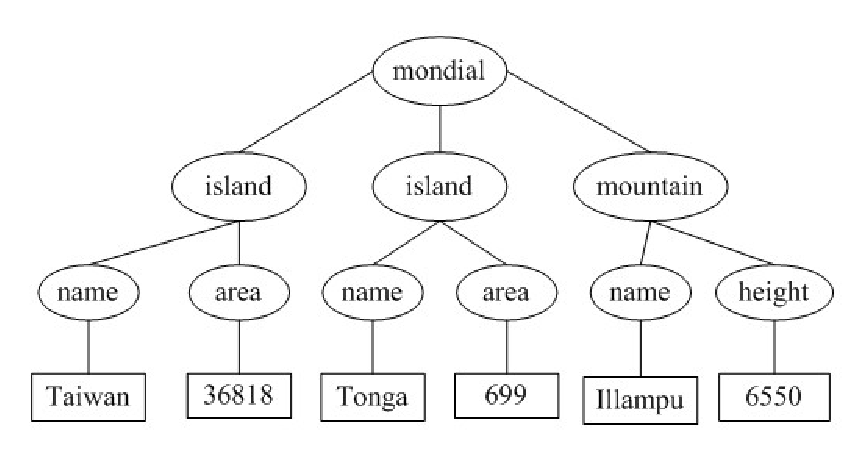
\includegraphics[width=0.4\textwidth]{XML}
\caption{树状结构}\label{fig:xml}
\vspace{\baselineskip}
\end{figure}


其插入图片的代码及其说明如下。
\vspace{1em}\noindent\hrule
\begin{verbatim}
\begin{figure}[htbp]
\centering
\includegraphics[width=0.4\textwidth]{文件名(.eps)}
\caption{标题}\label{标签名(通常为 fig:labelname)}
\vspace{\baselineskip} %表示图与正文空一行
\end{figure}
\end{verbatim}

\noindent\hrule

\begin{verbatim}
figure环境的可选参数[htbp]表示浮动图形所放置的位置,h (here)表示当前位置,t (top)表示页芯顶部,b (bottom)表示页芯底部,p (page)表示单独一页。在Word等软件中,图片通常插入到当前位置,如果当前页的剩余空间不够,图片将被移动到下一页,当前页就会出现很大的空白,其人工调整工作非常不便。由LaTeX提供的浮动图片功能,总是会按h->t->b->p的次序处理选项中的字母,自动调整图片的位置,大大减轻了工作量。
\centering命令将后续内容转换成每行皆居中的格式。
"\includegraphics"的可选参数用来设置图片插入文中的水平宽度,一般表示为正文宽度(\textwidth)的倍数。
\caption命令可选参数“标签名”为英文形式,一般不以图片或表格的数字顺序作为标签,而应包含一定的图片或表格信息,以便于文中引用(若图片、表格、公式、章节和参考文献等在文中出现的先后顺序发生了变化,其标注序号及其文中引用序号也会跟着发生变化,这一点是Word等软件所不能做到的)。另外,图题或表题并不会因为分页而与图片或表格体分置于两页,章节等各级标题也不会置于某页的最底部,LaTeX系统会自动调整它们在正文中的位置,这也是Word等软件所无法匹敌的。
\vspace将产生一定高度的竖直空白,必选参数为负值表示将后续文字位置向上提升,参数值可自行调整。em为长度单位,相当于大写字母M的宽度。\vspace{\baselineskip} 表示图与正文空一行。
引用方法:“见图~\ref{fig:figname}”、“如图~\ref{fig:figname}~所示”等。
\end{verbatim}

\noindent\hrule\vspace{1em}

若需要将~2~张及以上的图片并排插入到一行中,则需要采用\verb|minipage|环境,如图~\ref{fig:dd}~和图~\ref{fig:ds}~所示。
\begin{figure}[htbp]
\centering
\begin{minipage}{0.4\textwidth}
\centering
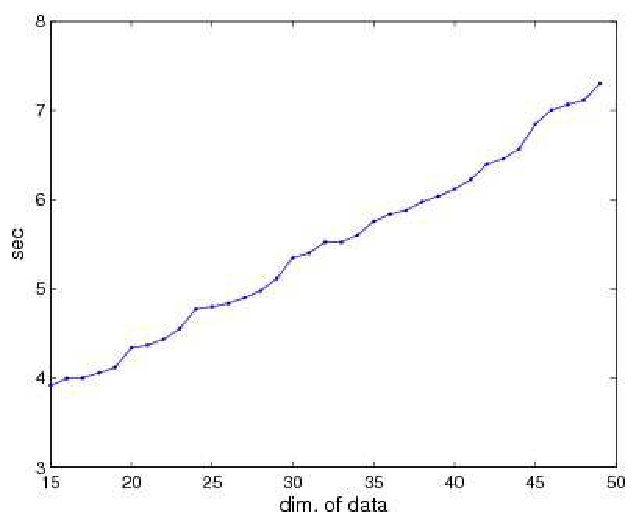
\includegraphics[width=\textwidth]{dataDimensions}
\caption{数据维数的变化}\label{fig:dd}
\end{minipage}
\begin{minipage}{0.4\textwidth}
\centering
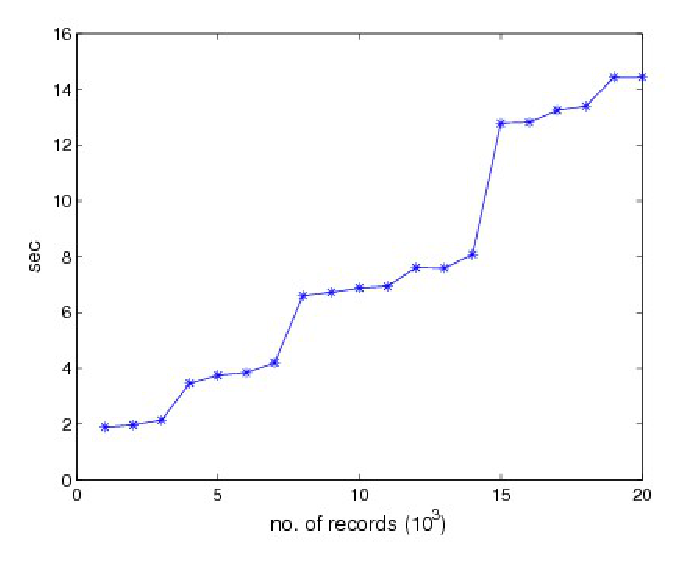
\includegraphics[width=\textwidth]{dataSize}
\caption{数据规模的变化}\label{fig:ds}
\end{minipage}
\vspace{\baselineskip}
\end{figure}

其代码如下所示。
\vspace{1em}\noindent\hrule
\begin{verbatim}
\begin{figure}[htbp]
\centering
\begin{minipage}{0.4\textwidth}
\centering
\includegraphics[width=\textwidth]{文件名}
\caption{标题}\label{fig:f1}
\end{minipage}
\begin{minipage}{0.4\textwidth}
\centering
\includegraphics[width=\textwidth]{文件名}
\caption{标题}\label{fig:f2}
\end{minipage}\vspace{\baselineskip}
\end{figure}
\end{verbatim}

\noindent\hrule

\begin{verbatim}
minipage环境的必选参数用来设置小页的宽度,若需要在一行中插入n个等宽图片,则每个小页的宽度应略小于(1/n)\textwidth。
\end{verbatim}

\noindent\hrule

\section{具有子图的图片插入方法}

图中若含有子图时,需要调用~subfigure~宏包, 如图~\ref{fig:subfig}~所示。
\begin{figure}[htbp]
  \centering
  \subfigure[Data Dimensions]{\label{fig:subfig:datadim}
                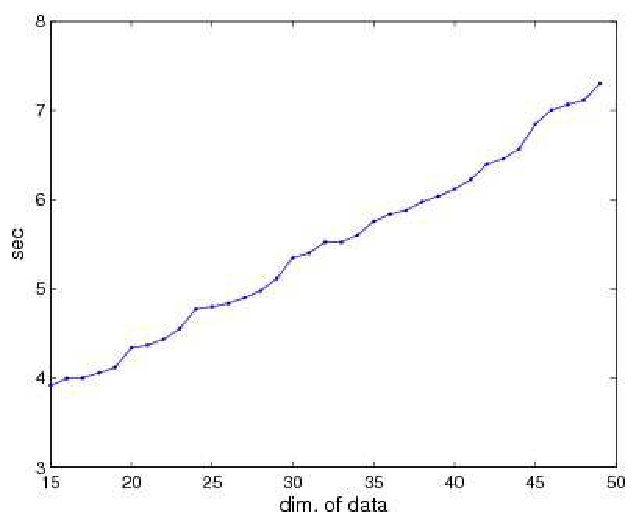
\includegraphics[width=0.4\textwidth]{dataDimensions}}
  \subfigure[Data Size]{\label{fig:subfig:datasize}
                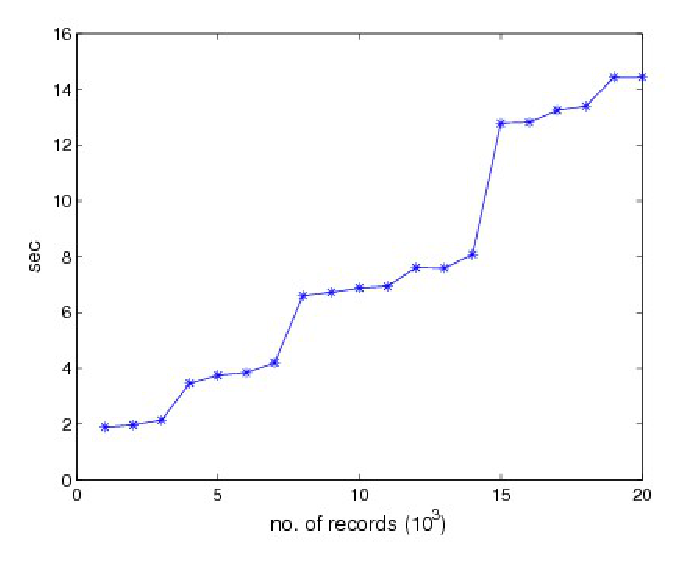
\includegraphics[width=0.4\textwidth]{dataSize}}
  \caption{Scalability of data}\label{fig:subfig}
\vspace{\baselineskip}
\end{figure}

其代码及其说明如下。
\vspace{1em}\noindent\hrule

\begin{verbatim}
\begin{figure}[htbp]
  \centering
  \subfigure[第1个子图标题]{
            \label{第1个子图标签(通常为 fig:subfig1:subsubfig1)}
            \includegraphics[width=0.4\textwidth]{文件名}}
  \subfigure[第2个子图标题]{
            \label{第2个子图标签(通常为 fig:subfig1:subsubfig2)}
            \includegraphics[width=0.4\textwidth]{文件名}}
  \caption{总标题}\label{总标签(通常为 fig:subfig1)}
\vspace{\baselineskip}
\end{figure}
\end{verbatim}

\noindent\hrule

\begin{verbatim}
子图的标签实际上可以随意设定,只要不重复就行。但为了更好的可读性,我们建议fig:subfig:subsubfig格式命名,这样我们从标签名就可以知道这是一个子图引用。
引用方法:总图的引用方法同本章第1节,子图的引用方法用\ref{fig:subfig:subsubfig}来代替。
\end{verbatim}

\noindent\hrule\vspace{1em}

子图的引用示例:如图~\ref{fig:subfig:datadim}~和图~\ref{fig:subfig:datasize}~所示。

若想获得插图方法的更多信息,参见网络上的~\href{ftp://ftp.tex.ac.uk/tex-archive/info/epslatex.pdf}{Using Imported Graphics in \LaTeX and pdf\LaTeX}~文档。 

\section{插入算法}

\begin{algorithm}[!h]
{
{
\renewcommand\baselinestretch{1.5}\selectfont %控制行距
\caption{ Scheduling Algorithm }
\label{alg:schedule}
\begin{algorithmic}[1]
\REQUIRE ~\\
A DFG $G=<V,E>$;\\
An allocation $A(G)$ for $G$.
\ENSURE ~\\
A schedule.
    \STATE{.......................}
    \FOR{$i\leftarrow\ 1\ to\ M$}    
        \STATE{.......................}
    \ENDFOR
    \STATE{.......................}
    \STATE{.......................}
    \STATE{.......................}
    \STATE{.......................}
    \STATE{.......................}
    \FOR{$k\leftarrow\ 1\ to\ |V|$}
        \STATE{.......................}
        \STATE{.......................}
        \STATE{.......................}
        \STATE{.......................}
    \IF{$LT_k==j$}
        \IF{there is no idle core in cluster $cl_{loc}$}
            \STATE{.......................}
            \STATE{.......................}
            \STATE{.......................}
            \STATE{.......................}
            \STATE{.......................}
            \STATE{.......................}
        \ELSE
            \STATE{.......................}
            \STATE{.......................}
            \STATE{.......................}
            \STATE{.......................}
            \STATE{.......................}
            \STATE{.......................}
        \ENDIF
    \ENDIF
    \ENDFOR
 

\end{algorithmic}
}
\par}
\end{algorithm}
%%% !Mode:: "TeX:UTF-8"

\chapter{表格的绘制方法}
\section{研究生毕业设计论文的绘表规范}

表应有自明性。表格不加左、右边线。表的编排建议采用国际通行的三线表。表内中文书写使用宋体五号字。

每个表格之上均应有表题(由表序和表名组成)。表序一般按章编排,如第~1~章第一个插表的序号为“表~1-1”等。表序与表名之间空两格,
表名使用中文五号字,居中。表名中不允许使用标点符号,表名后不加标点。
表头设计应简单明了,尽量不用斜线。表头中可采用化学,物理量等专业符号。

全表如用同一单位,则将单位符号移至表头右上角,加圆括号\cite{djy}。
表中数据应准确无误,书写清楚。数字空缺的格内加横线“-”(占~2~个数字宽度)。表内文字或数字上、下或左、右相同时,
采用通栏处理方式,不允许用“〃”、“同上”之类的写法。

表内文字使用宋体五号字,垂直居中书写,起行空一格、转行顶格、句末不加标点。
如某个表需要转页接排,在随后的各页上应重复表的编号。编号后加“(续表)”,表题可省略。续表应重复表头。
表格绘制完成之后,与正文空一行。

\section{普通表格的绘制方法}

表格应具有三线表格式,因此需要调用~booktabs~宏包,其标准格式如表~\ref{tab:table1}~所示。

\renewcommand\arraystretch{1.5}%控制行距
\begin{table}[!h]
\caption{基准测试集参数}\label{tab:bench}
\vspace{0.5em}
\centering
\begin{tabular}{l*{1}{C{2cm}}*{1}{L{6.2cm}}}
\toprule
Name         & $n$ & Description\\
\midrule
Random1      & 50  & Random graph generated by TGFF\\
Random2      & 100 & Random graph generated by TGFF\\
Random3      & 150 & Random graph generated by TGFF\\
Random4      & 200 & Random graph generated by TGFF\\
Random5      & 250 & Random graph generated by TGFF\\
Random6      & 300 & Random graph generated by TGFF\\
Random7      & 350 & Random graph generated by TGFF\\
Random8      & 400 & Random graph generated by TGFF\\
Random9      & 450 & Random graph generated by TGFF\\
Random10     & 500 & Random graph generated by TGFF\\
\bottomrule
\end{tabular}
\vspace{\baselineskip}
\end{table}
\renewcommand\arraystretch{1}

其绘制表格的代码及其说明如下。
\vspace{1em}\noindent\hrule

\begin{verbatim}
\begin{table}[htbp]
\caption{表标题}\label{标签名(通常为 tab:tablename)}
\vspace{0.5em}\centering\wuhao
\begin{tabular}{cc...c}
\toprule[1.5pt]
表头第1个格   & 表头第2个格   & ... & 表头第n个格  \\
\midrule[1pt]
表中数据(1,1) & 表中数据(1,2) & ... & 表中数据(1,n)\\
表中数据(2,1) & 表中数据(2,2) & ... & 表中数据(2,n)\\
表中数据(3,1) & 表中数据(3,2) & ... & 表中数据(3,n)\\
表中数据(4,1) & 表中数据(4,2) & ... & 表中数据(4,n)\\
...................................................\\
表中数据(m,1) & 表中数据(m,2) & ... & 表中数据(m,n)\\
\bottomrule[1.5pt]
\end{tabular}
\vspace{\baselineskip}
\end{table}
\end{verbatim}

\noindent\hrule

\begin{verbatim}
table环境是一个将表格嵌入文本的浮动环境。
\wuhao命令将表格的字号设置为五号字(10.5pt),在绘制表格结束退出时,不需要将字号再改回为\xiaosi,正文字号默认为小四号字(12pt)。
tabular环境的必选参数由每列对应一个格式字符所组成:c表示居中,l表示左对齐,r表示右对齐,其总个数应与表的列数相同。此外,@{文本}可以出现在任意两个上述的列格式之间,其中的文本将被插入每一行的同一位置。表格的各行以\\分隔,同一行的各列则以&分隔。
\toprule、\midrule和\bottomrule三个命令是由booktabs宏包提供的,其中\toprule和\bottomrule分别用来绘制表格的第一条(表格最顶部)和第三条(表格最底部)水平线,\midrule用来绘制第二条(表头之下)水平线,且第一条和第三条水平线的线宽为1.5pt,第二条水平线的线宽为1pt。
引用方法:“如表~\ref{tab:tablename}~所示”。
\end{verbatim}

\noindent\hrule

\section{长表格的绘制方法}

长表格是当表格在当前页排不下而需要转页接排的情况下所采用的一种表格环境。若长表格仍按照普通表格的绘制方法来获得,
其所使用的\verb|table|浮动环境无法实现表格的换页接排功能,表格下方过长部分会排在表格第1页的页脚以下。为了能够实现长表格的转页接排功能,
需要调用~longtable~宏包,由于长表格是跨页的文本内容,因此只需要单独的\verb|longtable|环境,所绘制的长表格的格式如表~\ref{tab:table2}~所示。

此长表格~\ref{tab:table2}~第~2~页的标题“编号(续表)”和表头是通过代码自动添加上去的,无需人工添加,若表格在页面中的竖直位置发生了变化,长表格在第~2~页
及之后各页的标题和表头位置能够始终处于各页的最顶部,也无需人工调整,\LaTeX~系统的这一优点是~Word~等软件所无法企及的。

下段内容是为了让下面的长表格分居两页,看到表标题“编号(续表)”的效果。摘录于《你若安好,便是晴天 -- 林徽因传》片段:

她叫林徽因,出生于杭州,是许多人梦中期待的白莲。她在雨雾之都伦敦,发生过一场空前绝后的康桥之恋。她爱过三个男子,爱得清醒,也爱得平静。徐志摩为她徜徉在康桥,深情地等待一场旧梦可以归来。梁思成与她携手走过千山万水,为完成使命而相约白头。金岳霖为她终身不娶,痴心不改地守候一世。可她懂得人生飘忽不定,要学会随遇而安。
真正的平静,不是避开车马喧嚣,而是在心中修篱种菊。尽管如流往事,每一天都涛声依旧,只要我们消除执念,便可寂静安然。愿每个人在纷呈世相中不会迷失荒径,可以端坐磐石上,醉倒落花前。
如果可以,请让我预支一段如莲的时光,哪怕将来某一天加倍偿还。这个雨季会在何时停歇,无从知晓。但我知道,你若安好,便是晴天。					 
\wuhao\begin{longtable}{ccc}
\caption{湖南大学各学院名称一览}\label{tab:table2}
 \vspace{0.5em}\\
\toprule[1.5pt] 学院名称 & 网址 & 联系电话  \\ \midrule[1pt]
\endfirsthead
\multicolumn{3}{c}{表~\thetable(续表)}\vspace{0.5em}\\
\toprule[1.5pt] 学院名称 & 网址 & 联系电话  \\ \midrule[1pt]
\endhead
\bottomrule[1.5pt]
\endfoot
机械工程学院& \url{http://tdjxxy.tju.edu.cn/}& 87401979\\
精密仪器与光电子工程学院&  \url{http://www2.tju.edu.cn/colleges/precision/cn/}& 27404775\\
电子信息工程学院& \url{http://www.tju.edu.cn/seie}& 27406956\\
电气与自动化工程学院& \url{http://www2.tju.edu.cn/colleges/automate/}& 27405477\\
建筑工程学院& \url{http://www2.tju.edu.cn/colleges/civil/}& 27404072\\
化工学院& \url{http://chemeng.tju.edu.cn/}& 27403389\\
材料科学与工程学院& \url{http://mse.tju.edu.cn}& 27406693 \\
建筑学院& \url{http://hgw022072.chinaw3.com/}& 27402724-2111\\
求是学部\\
管理与经济学部&	\url{ http://sm.tju.edu.cn}& 27403423\\
理学院& \url{ http://www.tju.edu.cn/science/}& 27404118\\
文法学院& \url{ http://www2.tju.edu.cn/colleges/sociology/new/}& 27403691\\
软件学院& \url{http://scs.tju.edu.cn}& 87401540\\
计算机科学与技术学院& \url{http://cs.tju.edu.cn/}& 27406538\\
马克思主义学院& \url{http://www2.tju.edu.cn/colleges/marxism/}& 27405348\\
环境科学与工程学院& \url{http://www.tju.edu.cn/see}& 87402072\\
药物科学与技术学院& \url{http://www2.tju.edu.cn/colleges/pharmtier/}& 87401830\\
教育学院& \url{http://soe.tju.edu.cn/}& 27401028\\
职业技术教育学院& \url{http://202.113.0.248:8888}\\
继续教育学院& \url{http://aectu.tju.edu.cn/}& 27406298\\
仁爱学院& \url{http://www.tjrac.edu.cn/}& 68579990\\
农业与生物工程学院& \url{http://202.113.13.169/site/nongxueyuan/}& 87402171\\
国际教育学院 & \url{http://www.ietju.com/}& 27406147\\
网络教育学院 & \url{http://www.etju.com/}& 27426952 \\

\end{longtable}\xiaosi
\vspace{\baselineskip}

绘制长表格的代码及其说明如下。
\vspace{1em}\noindent\hrule

\begin{verbatim}
\wuhao\begin{longtable}{cc...c}
\caption{表标题}\label{标签名(通常为 tab:tablename)}\\
\toprule[1.5pt] 表头第1个格 & 表头第2个格 & ... & 表头第n个格\\ \midrule[1pt]
\endfirsthead
\multicolumn{n}{c}{表~\thetable(续表)}\vspace{0.5em}\\
\toprule[1.5pt] 表头第1个格 & 表头第2个格 & ... & 表头第n个格\\ \midrule[1pt]
\endhead
\bottomrule[1.5pt]
\endfoot
表中数据(1,1) & 表中数据(1,2) & ... & 表中数据(1,n)\\
表中数据(2,1) & 表中数据(2,2) & ... & 表中数据(2,n)\\
...................................................\\
表中数据(m,1) & 表中数据(m,2) & ... & 表中数据(m,n)\\
\end{longtable}\xiaosi
\end{verbatim}

\noindent\hrule
\begin{verbatim}
在绘制长表格的前面留出一个空白行,并在第2行的一开始全局定义长表格的字号为五号字,这样能够保证长表格之前段落的行距保持不变。
在绘制长表格结束后,需要\xiaosi命令重新将字号改为小四号字。
\endhead之前的文字描述的是第2页及其之后各页的标题或表头;
\endfirsthead之前的文字描述的是第1页的标题和表头,若无此命令,则第1页的表头和标题由\endhead命令确定;
同理,\endfoot之前的文字描述的是除最后一页之外每页的表格底部内容;
\endlastfoot之前的文字描述的是最后一页的表格底部内容,若无此命令,
则最后一页的表格底部内容由\endfoot命令确定;由于规范中长表格每页底部内容均相同(水平粗线),因此模板中没有用到\endlastfoot命令。
\end{verbatim}

\noindent\hrule
\section{列宽可调表格的绘制方法}
论文中能用到列宽可调表格的情况共有两种:一种是当插入的表格某一单元格内容过长以至于一行放不下的情况,
另一种是当对公式中首次出现的物理量符号进行注释的情况。这两种情况都需要调用~tabularx~宏包。下面将分别对这两种情况下可调表格的绘制方法进行阐述。
\subsection{表格内某单元格内容过长的情况}

首先给出这种情况下的一个例子如表~\ref{tab:table3}~所示。
\begin{table}[htbp]
\caption{最小的三个正整数的英文表示法}\label{tab:table3}
\vspace{0.5em}\wuhao
\begin{tabularx}{\textwidth}{llX}
\toprule[1.5pt]
Value & Name & Alternate names, and names for sets of the given size\\\midrule[1pt]
1 & One & ace, single, singleton, unary, unit, unity\\
2 & Two & binary, brace, couple, couplet, distich, deuce, double, doubleton, duad, duality, duet, duo, dyad, pair, snake eyes, span, twain, twosome, yoke\\
3 & Three & deuce-ace, leash, set, tercet, ternary, ternion, terzetto, threesome, tierce, trey, triad, trine, trinity, trio, triplet, troika, hat-trick\\\bottomrule[1.5pt]
\end{tabularx}
\vspace{\baselineskip}
\end{table}
绘制这种表格的代码及其说明如下。
\vspace{1em}\noindent\hrule
\begin{verbatim}
\begin{table}[htbp]
\caption{表标题}\label{标签名(通常为 tab:tablename)}
\vspace{0.5em}\wuhao
\begin{tabularx}{\textwidth}{l...X...l}
\toprule[1.5pt]
表头第1个格   & ... & 表头第X个格   & ... & 表头第n个格  \\
\midrule[1pt]
表中数据(1,1) & ... & 表中数据(1,X) & ... & 表中数据(1,n)\\
表中数据(2,1) & ... & 表中数据(2,X) & ... & 表中数据(2,n)\\
.........................................................\\
表中数据(m,1) & ... & 表中数据(m,X) & ... & 表中数据(m,n)\\
\bottomrule[1.5pt]
\end{tabularx}
\vspace{\baselineskip}
\end{table}
\end{verbatim}

\noindent\hrule
\begin{verbatim}
tabularx环境共有两个必选参数:第1个参数用来确定表格的总宽度,这里取为排版表格能达到的最大宽度——正文宽度\textwidth;第2个参数用来确定每列格式,其中标为X的项表示该列的宽度可调,其宽度值由表格总宽度确定。
标为X的列一般选为单元格内容过长而无法置于一行的列,这样使得该列内容能够根据表格总宽度自动分行。若列格式中存在不止一个X项,则这些标为X的列的列宽相同,因此,一般不将内容较短的列设为X。
标为X的列均为左对齐,因此其余列一般选为l(左对齐),这样可使得表格美观,但也可以选为c或r。
\end{verbatim}

\noindent\hrule
\subsection{对物理量符号进行注释的情况}
为使得对公式中物理量符号注释的转行与破折号“———”后第一个字对齐,此处最好采用表格环境。此表格无任何线条,左对齐,
且在破折号处对齐,一共有“式中”二字、物理量符号和注释三列,表格的总宽度可选为文本宽度,因此应该采用\verb|tabularx|环境。
由\verb|tabularx|环境生成的对公式中物理量符号进行注释的公式如式(\ref{eq:1})所示。
%\vspace*{10pt}

\begin{equation}\label{eq:1}
\ddot{\boldsymbol{\rho}}-\frac{\mu}{R_{t}^{3}}\left(3\mathbf{R_{t}}\frac{\mathbf{R_{t}\rho}}{R_{t}^{2}}-\boldsymbol{\rho}\right)=\mathbf{a}
\end{equation}

\begin{tabularx}{\textwidth}{@{}l@{\quad}r@{———}X@{}}
式中& $\bm{\rho}$ &追踪飞行器与目标飞行器之间的相对位置矢量;\\
&  $\bm{\ddot{\rho}}$&追踪飞行器与目标飞行器之间的相对加速度;\\
&  $\mathbf{a}$   &推力所产生的加速度;\\
&  $\mathbf{R_t}$ & 目标飞行器在惯性坐标系中的位置矢量;\\
&  $\omega_{t}$ & 目标飞行器的轨道角速度;\\
&  $\mathbf{g}$ & 重力加速度,$=\frac{\mu}{R_{t}^{3}}\left(
3\mathbf{R_{t}}\frac{\mathbf{R_{t}\rho}}{R_{t}^{2}}-\bm{\rho}\right)=\omega_{t}^{2}\frac{R_{t}}{p}\left(
3\mathbf{R_{t}}\frac{\mathbf{R_{t}\rho}}{R_{t}^{2}}-\bm{\rho}\right)$,这里~$p$~是目标飞行器的轨道半通径。
\end{tabularx}
\vspace{\wordsep}

其中生成注释部分的代码及其说明如下。

\vspace{1em}\noindent\hrule

\begin{verbatim}
\begin{tabularx}{\textwidth}{@{}l@{\quad}r@{— — —}X@{}}
式中 & symbol-1 & symbol-1的注释内容;\\
     & symbol-2 & symbol-2的注释内容;\\
     .............................;\\
     & symbol-m & symbol-m的注释内容。
\end{tabularx}\vspace{\wordsep}
\end{verbatim}

\noindent\hrule

\begin{verbatim}
tabularx环境的第1个参数选为正文宽度,第2个参数里面各个符号的意义为:
    第1个@{}表示在“式中”二字左侧不插入任何文本,“式中”二字能够在正文中左对齐,若无此项,则“式中”二字左侧会留出一定的空白;
    @{\quad}表示在“式中”和物理量符号间插入一个空铅宽度的空白;
    @{— — —}实现插入破折号的功能,它由三个1/2的中文破折号构成;
    第2个@{}表示在注释内容靠近正文右边界的地方能够实现右对齐。
\end{verbatim}

\noindent\hrule\vspace{1em}

由此方法生成的注释内容应紧邻待注释公式并置于其下方,因此不能将代码放入\verb|table|浮动环境中。但此方法不能实现自动转页接排,
可能会在当前页剩余空间不够时,全部移动到下一页而导致当前页出现很大空白。因此在需要转页处理时,还请您手动将需要转页的代码放入一个
新的\verb|tabularx|环境中,将原来的一个\verb|tabularx|环境拆分为两个\verb|tabularx|环境。

若想获得绘制表格的更多信息,参见网络上的~\href{http://www.tug.org/pracjourn/2007-1/mori/}{Tables in \LaTeXe: Packages and Methods}~文档。


%%% !Mode:: "TeX:UTF-8"

\chapter{数学公式的输入方法}
\section{研究生毕业设计论文的公式规范}

论文中的公式应另起行,原则上应居中书写,与周围文字留有足够的空间区分开。
若公式前有文字(如“解”、“假定”等),文字空两格写,公式仍居中写。公式末不加标点。

公式应标注序号,并将序号置于括号内。 公式序号按章编排,如第~1~章第一个公式序号为“(1-1)”。公式的序号右端对齐。

公式较长时最好在等号“=”处转行,如难实现,则可在~$+$、$-$、$\times$、$\div$~运算符号处转行,转行时运算符号仅书写于转行式前,不重复书写。

文中引用公式时,一般用“见式~(1-1)”或“由公式~(1-1)”。

公式中用斜线表示“除”的关系时应采用括号,以免含糊不清,如~$a/(b\cos x)$。通常“乘”的关系在前,如~$a\cos x/b$而不写成~$(a/b)\cos x$。

不能用文字形式表示等式,如:$\textnormal{刚度}=\frac{{\textnormal{受力}}}{{\textnormal{受力方向的位移}}}$。

对于数学公式的输入方法,网络上有一个比较全面权威的文档\textbf{~\href{http://tug.ctan.org/cgi-bin/ctanPackageInformation.py?id=voss-mathmode}{Math mode}}~请大家事先大概浏览一下。下面将对学位论文中主要用到的数学公式排版形式进行阐述。

\section{生成~\LaTeX~数学公式的两种方法}
对于先前没有接触过~\LaTeX~的人来说,编写~\LaTeX~数学公式是一件很繁琐的事,尤其是对复杂的数学公式来说,更可以说是一件难以完成的任务。
实际上,生成~\LaTeX~数学公式有两种较为简便的方法,一种是基于~MathType~数学公式编辑器的方法,另一种是基于~MATLAB~商业数学软件的方法,
下面将分别对这两种数学公式的生成方法作一下简单介绍。

\subsection{基于~MathType~软件的数学公式生成方法}
MathType~是一款功能强大的数学公式编辑器软件,能够用来在文本环境中插入~Windows OLE~图形格式的复杂数学公式,所以应用比较普遍。但此软件只有~30~天的试用期,之后若再继续使用则需要付费购买才行。网络上有很多破解版的~MathType~软件可供下载免费使用,
笔者推荐下载安装版本号在~6.5~之上的中文破解版。

在安装好~MathType~之后,若在输入窗口中编写数学公式,复制到剪贴板上的仍然是图形格式的对象。
若希望得到可插入到~\LaTeX~编辑器中的文本格式对象,则需要对~MathType~软件做一下简单的设置:在~MathType~最上排的按钮中依次选择“参数选项
$\to$转换”,在弹出的对话窗中选中“转换到其它语言(文字):”,在转换下拉框中选择“Tex~--~--~LaTeX 2.09 and later”,并将对话框最下方的两个复选框全部勾掉,点击确定,这样,再从输入窗口中复制出来的对象就是文本格式的了,就可以直接将其粘贴到~\LaTeX~
编辑器中了。按照这种方法生成的数学公式两端分别有标记\verb|\[|和标记\verb|\]|,在这两个标记之间才是真正的数学公式代码。

若希望从~MathType~输入窗口中复制出来的对象为图形格式,则只需再选中“公示对象(Windows OLE~图形)”即可。

\subsection{基于~MATLAB~软件的数学公式生成方法}

MATLAB~是矩阵实验室(Matrix Laboratory)的简称,是美国~MathWorks~公司出品的商业数学软件。它是当今科研领域最常用的应用软件之一,
具有强大的矩阵计算、符号运算和数据可视化功能,是一种简单易用、可扩展的系统开发环境和平台。

MATLAB~中提供了一个~latex~函数,它可将符号表达式转化为~\LaTeX~数学公式的形式。其语法形式为~latex(s),其中,~s~为符号表达式,
之后再将~latex~函数的运算结果直接粘贴到~\LaTeX~编辑器中。从~\LaTeX~数学公式中可以发现,其中可能包含如下符号组合:

\begin{verbatim*}
\qquad=两个空铅(quad)宽度
\quad=一个空铅宽度
\;=5/18空铅宽度
\:=4/18空铅宽度
\,=3/18空铅宽度
\!=-3/18空铅宽度
\ =一个空格
\end{verbatim*}

所以最好将上述符号组合从数学公式中删除,从而使数学公式显得匀称美观。

对于~Word~等软件的使用者来说,在我们通过~MATLAB~运算得到符号表达式形式的运算结果时,在~Word~中插入运算结果需要借助于~MathType~软件,
通过在~MathType~中输入和~MATLAB~运算结果相对应的数学表达形式,之后再将~MathType~数学表达式转换为图形格式粘贴到~Word~中。实际上,
也可以将~MATLAB~中采用~latex~函数运行的结果直接粘贴到~MathType~中,再继续上述步骤,这样可以大大节省输入公式所需要的时间。
此方法在~MathType~6.5c~上验证通过,若您粘入到~MathType~中的仍然为从~MATLAB~中导入的代码,请您更新~MathType~软件。

\section{数学字体}
在数学模式下,常用的数学字体命令有如下几种:

\begin{verbatim}
\mathnormal或无命令 用数学字体打印文本;
\mathit             用斜体(\itshape)打印文本;
\mathbf             用粗体(\bfseries)打印文本;
\mathrm             用罗马体(\rmfamily)打印文本;
\mathsf             用无衬线字体(\sffamily)打印文本;
\mathtt             用打印机字体(\ttfamily)打印文本;
\mathcal            用书写体打印文本;
\end{verbatim}

在学位论文撰写中,只需要用到上面提到的~\verb|\mathit|、\verb|\mathbf|~和~\verb|\mathrm|~命令。若要得到~Times New Roman~的数学字体,则需要调用~txfonts~宏包(此宏包实际上采用的是~Nimbus Roman No9 L~字体,
它是开源系统中使用的免费字体,其字符字体与~Times New Roman~字体几乎完全相同);若要得到粗体数学字体,则需要调用~bm~宏包。表~\ref{tab:fonts}~中分别列出了得到阿拉伯数字、拉丁字母和希腊字母
各种数学字体的命令。

\begin{table}[htbp]
\caption{常用数学字体命令一览}\label{tab:fonts}
\vspace{0.5em}\centering\wuhao
\begin{tabular}{llll}
\toprule
 & 阿拉伯数字\&大写希腊字母 & 大小写拉丁字母 & 小写希腊字母  \\
\midrule
斜体 & \verb|\mathit{}| & \verb|无命令| & \verb|无命令|\\
粗斜体 & \verb|\bm{\mathit{}}| & \verb|\bm{}| & \verb|\bm{}|\\
直立体 & \verb|无命令| & \verb|\mathrm{}| & \verb|字母后加up|\\
粗体 & \verb|\mathbf{}或\bm{}| & \verb|\mathbf{}| & \verb|\bm{字母后加up}|\\
\bottomrule
\end{tabular}
\vspace{\baselineskip}
\end{table}

\noindent 下面列出了一些应采用直立数学字体的数学常数和数学符号。

\vspace{-0.5em}\begin{center}\begin{tabularx}{0.7\textwidth}{XX}
$\mathrm{d}$、 $\mathrm{D}$、 $\mathrm{p}$~———微分算子 & $\mathrm{e}$~———自然对数之底数\\
$\mathrm{i}$、 $\mathrm{j}$~———虚数单位 & $\piup$———圆周率\\
\end{tabularx}\end{center}

\section{行内公式}
出现在正文一行之内的公式称为行内公式,例如~$f(x)=\int_{a}^{b}\frac{\sin{x}}{x}\mathrm{d}x$。对于非矩阵和非多行形式的行内公式,一般不会使得行距发生变化,而~Word~等软件却会根据行内公式的竖直距离而自动调节行距,如图~\ref{fig:hangju}~所示。

\begin{figure}[htbp]
\centering
\subfigure[由~\LaTeX~系统生成的行内公式]{\label{fig:subfig:latex}
                \fbox{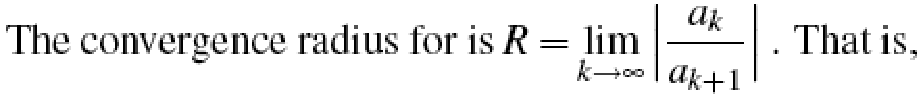
\includegraphics[width=0.55\textwidth]{latex}}}
\subfigure[由~Word软件生成的~.doc~格式行内公式]{\label{fig:subfig:word}
                \fbox{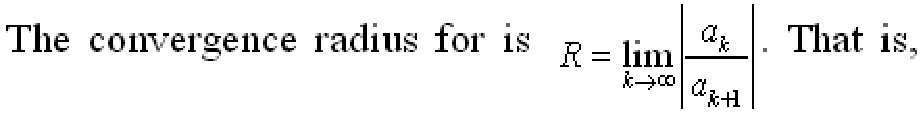
\includegraphics[width=0.55\textwidth]{word}}}
\subfigure[由~Word软件生成的~.pdf~格式行内公式]{\label{fig:subfig:pdf}
                \fbox{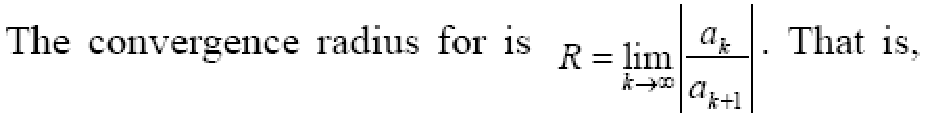
\includegraphics[width=0.55\textwidth]{pdf}}}

\caption{由~\LaTeX~和~Word~生成的~3~种行内公式屏显效果}\label{fig:hangju}
\vspace{-1em}
\end{figure}

这三幅图分别为~\LaTeX~和~Word~生成的行内公式屏显效果,从图中可看出,在~\LaTeX~文本含有公式的行内,在正文与公式之间对接工整,行距不变;而在~Word~文本含有公式的行内,在正文与公式之间对接不齐,行距变大。因此从这一点来说,
\LaTeX~系统在数学公式的排版上具有很大优势。

\LaTeX~提供的行内公式最简单、最有效的方法是采用~\TeX~本来的标记———开始和结束标记都写作~\$,例如本段开始的例子可由下面的输入得到。
\verb|$f(x)=\int_{a}^{b}\frac{\sin{x}}{x}\mathrm{d}x$|

\section{行间公式}
位于两行之间的公式称为行间公式,每个公式都是一个单独的段落,例如
\[\int_a^b{f\left(x\right)\mathrm{d}x}=\lim_{\left\|\Delta{x_i}\right\|\to 0}\sum_i{f\left(\xi_i\right)\Delta{x_i}}\]
除人工编号外,\LaTeX~各种类型行间公式的标记见表~\ref{tab:eqtag}。
\begin{table}[htbp]
\caption{各种类型行间公式的标记}\label{tab:eqtag}
\vspace{0.5em}\centering\wuhao
\begin{tabularx}{\textwidth}{cll}
\toprule
& 无编号 & 自动编号\\
\midrule
单行公式& \verb|\begin{displaymath}... \end{displaymath}|& \verb|\begin{equation}... \end{equation}|\\
        & 或~\verb|\[...\]| & \\
多行公式& \verb|\begin{eqnarray*}... \end{eqnarray*}|& \verb|\begin{eqnarray}... \end{eqnarray}|\\
\bottomrule
\end{tabularx}
\end{table}

另外,在自动编号的某行公式行尾添加标签~\verb|\nonumber|,可将该行转换为无编号形式。

行间多行公式需采用~\verb|eqnarray|~或~\verb|eqnarray*|~环境,它默认是一个列格式为~\verb|rcl|~的~3~列矩阵,并且中间列的字号要小一些,因此通常只将需要对齐的运算符号(通常为等号“=”)置于中间列。

\section{可自动调整大小的定界符}
若在左右两个定界符之前分别添加命令~\verb|\left|~和~\verb|\right|,则定界符可根据所包围公式大小自动调整其尺寸,这可从式(\ref{nodelimiter})和式(\ref{delimiter})中看出。
\begin{equation}\label{nodelimiter}
(\sum_{k=\frac12}^{N^2})
\end{equation}
\begin{equation}\label{delimiter}
\left(\sum_{k=\frac12}^{N^2}\right)
\end{equation}
式(\ref{nodelimiter})和式(\ref{delimiter})是在~\LaTeX~中分别输入如下代码得到的。
\begin{verbatim}
(\sum_{k=\frac12}^{N^2})
\left(\sum_{k=\frac12}^{N^2}\right)
\end{verbatim}
\verb|\left|~和~\verb|\right|~总是成对出现的,若只需在公式一侧有可自动调整大小的定界符,则只要用“.”代替另一侧那个无需打印出来的定界符即可。

若想获得关于此部分内容的更多信息,可参见~\href{http://tug.ctan.org/cgi-bin/ctanPackageInformation.py?id=voss-mathmode}{Math mode}~文档的第~8~章“Brackets, braces and parentheses”。

\section{数学重音符号}
数学重音符号通常用来区分同一字母表示的不同变量,输入方法如下(需要调用~\verb|amsmath|~宏包):

\vspace{0.5em}\noindent\wuhao\begin{tabularx}{\textwidth}{Xc|Xc|Xc}
 \verb|\acute| & $\acute{a}$ & \verb|\mathring| & $\mathring{a}$ & \verb|\underbrace| & $\underbrace{a}$ \\
 \verb|\bar| & $\bar{a}$ & \verb|\overbrace| & $\overbrace{a}$ & \verb|\underleftarrow| & $\underleftarrow{a}$ \\
 \verb|\breve| & $\breve{a}$ & \verb|\overleftarrow| & $\overleftarrow{a}$ & \verb|\underleftrightarrow| & $\underleftrightarrow{a}$ \\
 \verb|\check| & $\check{a}$ & \verb|\overleftrightarrow| & $\overleftrightarrow{a}$ & \verb|\underline| & $\underline{a}$ \\
 \verb|\dddot| & $\dddot{a}$ & \verb|\overline| & $\overline{a}$ & \verb|\underrightarrow| & $\underrightarrow{a}$ \\
 \verb|\ddot| & $\ddot{a}$ & \verb|\overrightarrow| & $\overrightarrow{a}$ & \verb|\vec| & $\vec{a}$ \\
 \verb|\dot| & $\dot{a}$ & \verb|\tilde| & $\tilde{a}$ & \verb|\widehat| & $\widehat{a}$ \\
 \verb|\grave| & $\grave{a}$ & \verb|\underbar| & $\underbar{a}$ & \verb|\widetilde| & $\widetilde{a}$ \\
 \verb|\hat| & $\hat{a}$
\end{tabularx}\vspace{0.5em}
\xiaosi 当需要在字母~$i$~和~$j$~的上方添加重音符号时,为了去掉这两个字母顶上的小点,这两个字母应该分别改用~\verb|\imath|~和~\verb|\jmath|。

如果遇到某些符号不知道该采用什么命令能输出它时,则可通过~\href{http://detexify.kirelabs.org/classify.html}{Detexify$^2$~网站}来获取符号命令。若用鼠标左键在此网页的方框区域内画出你所要找的符号形状,则会在网页右方列出和你所画符号形状相近的~5~个符号及其相对应的~\LaTeX~输入命令。若所列出的符号中不包括你所要找的符号,还可通过点击“Select from the complete list!”的链接以得分从低到高的顺序列出所有符号及其相对应的~\LaTeX~输入命令。

最后,建议大家还以~\href{http://tug.ctan.org/cgi-bin/ctanPackageInformation.py?id=voss-mathmode}{Math mode}~这篇~pdf~文档作为主要参考。若要获得最为标准、美观的数学公式排版形式,可以查查文档中是否有和你所要的排版形式相同或相近的代码段,通过修改代码段以获得你所要的数学公式排版形式。


%%% !Mode:: "TeX:UTF-8"

\chapter{罗列和定理环境使用方法}

\section{单层罗列环境}
湖南大学学位论文一般可采用两种罗列环境:一种是并列条目有同样标签的~\verb|itemize|~罗列环境,另一种是具有自动排序编号符号的~\verb|enumerate|~罗列环境。这两种罗列环境的样式参数可参考图~\ref{fig:list}。
\begin{figure}[htbp]
\centering
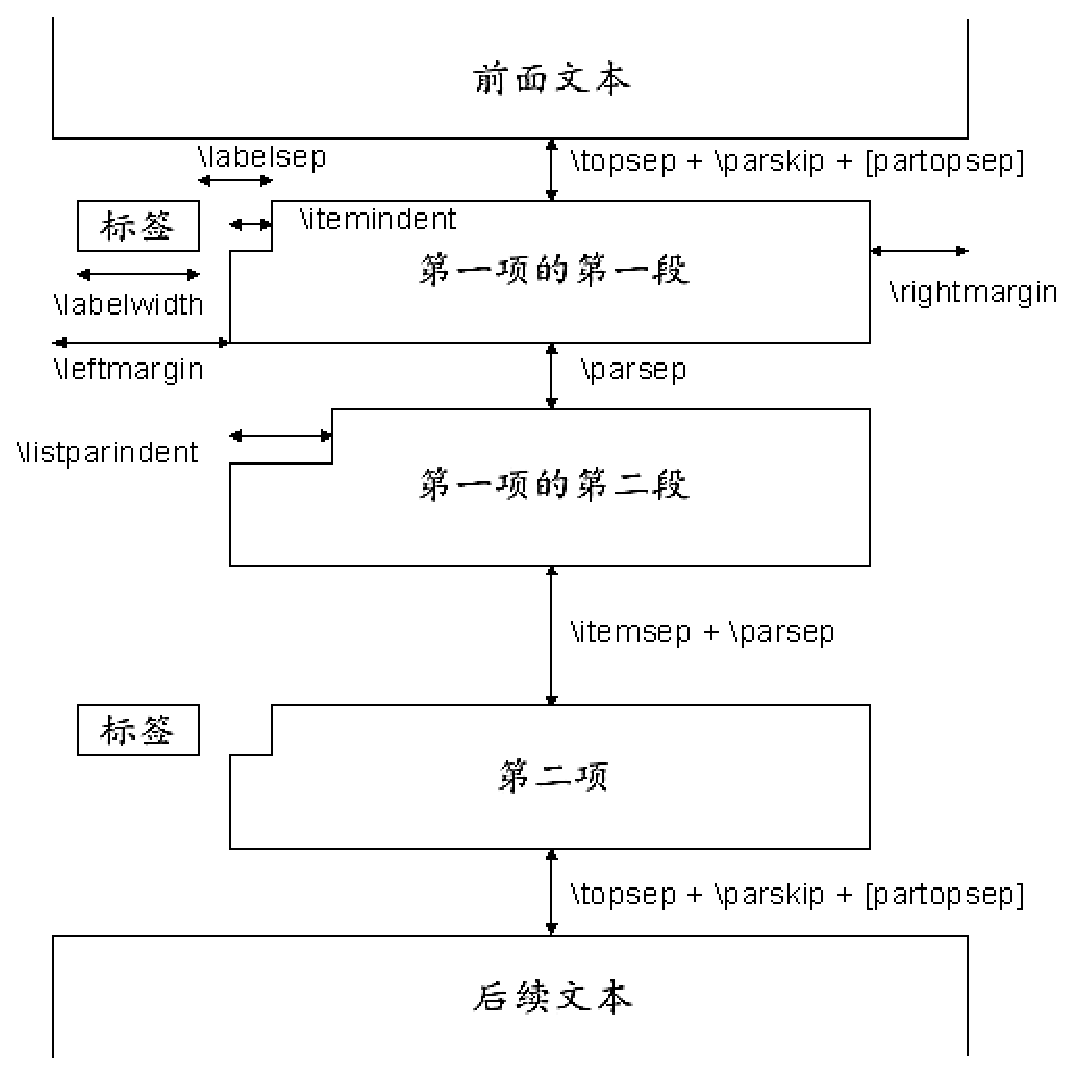
\includegraphics[width = 0.6\textwidth]{list}
\caption{罗列环境参数示意图}\label{fig:list}\vspace{-1em}
\end{figure}

通过调用~enumitem~宏包可以很方便地控制罗列环境的布局,其~format.tex~文件中的~\verb|\setitemize|~和~\verb|\setenumerate|~命令分别用来设置~\verb|itemize|~和~\verb|enumerate|~环境的样式参数。采用~\verb|itemize|~单层罗列环境的排版形式如下:

\begin{itemize}
\item 第一个条目文本内容
\item 第二个条目文本内容
\item 第三个条目文本内容
\end{itemize}

其代码如下

\begin{verbatim}
\begin{itemize}
  \item 第一个条目文本内容
  \item 第二个条目文本内容
  ...
  \item 第三个条目文本内容
\end{itemize}
\end{verbatim}

采用~\verb|enumerate|~单层罗列环境的排版形式如下:

\begin{enumerate}
\item 第一个条目文本内容
\item 第二个条目文本内容
\item 第三个条目文本内容
\end{enumerate}

其代码如下

\begin{verbatim}
\begin{enumerate}
  \item 第一个条目文本内容
  \item 第二个条目文本内容
  ...
  \item 第三个条目文本内容
\end{enumerate}
\end{verbatim}



\section{定理环境}

\begin{definition}[谱半径]\label{def:def1}
  称~$n$~阶方阵~$\mathbf{A}$~的全体特征值~$\lambda_1,\cdots,\lambda_n$~组成的集合为~$\mathbf{A}$~的谱,称
  $$\rho(\mathbf{A})=\max{\{|\lambda_1|,\cdots,|\lambda_n|\}}$$
\end{definition}
\begin{theorem}[相似充要条件]\label{lemma:l1}
  方阵$A$和$B$相似的充要条件是:~$A$~和~$B$~有全同的不变因子。
\end{theorem}
\begin{corollary}[推论1]\label{cor:cor1}
在赋范空间~$(X,\|\cdot\|)$~上定义~$d(x,y)=\|x-y\|$, 对任意~$x,y\in X$,~则~$(X,d)$~是距离空间。
\end{corollary}
\begin{proof}
  只需证明~$d(x,y)$~是距离。
\end{proof}
\newpage

定义代码如下:
\begin{verbatim}
 \begin{definition}[谱半径]\label{def:def1}
  称~$n$~阶方阵~$\mathbf{A}$~的全体特征值
  $\lambda_1,\cdots,\lambda_n$组成的集合为~$\mathbf{A}$~的谱,称
  $$\rho(\mathbf{A})=\max{\{|\lambda_1|,\cdots,|\lambda_n|\}}$$
\end{definition}
\end{verbatim}
\noindent\hrule

\vspace{0.1em}\noindent\hrule
\vspace{1em}
定理代码如下:
\begin{verbatim}
\begin{theorem}[相似充要条件]\label{lemma:l1}
  方阵$A$和$B$相似的充要条件是:$A$和$B$有全同的不变因子。
\end{theorem}
\end{verbatim}
\noindent\hrule\vspace{0.1em}

\noindent\hrule
\vspace{1em}
推论和证明代码如下:
\begin{verbatim}
\begin{corollary}[推论1]\label{cor:cor1}
在赋范空间~$(X,\|\cdot\|)$~上定义$d(x,y)=\|x-y\|$,
对任意$x,y\in X$,则$(X,d)$是距离空间。
\end{corollary}
\begin{proof}
  只需证明$d(x,y)$是距离。
\end{proof}
\end{verbatim}
\noindent\hrule\vspace{1em}

定理定义[]中是可选参数,用来说明定理的名称。其他环境格式书写与上面定理、定义、推论格式相同,可自己调用其他环境。
若需要书写定理定义等内容,而且带有顺序编号,需要采用如下环境。除了~\verb|proof|~环境之外,其余~9~个环境都可以有一个可选参数作为附加标题。

\begin{center}
\vspace{0.5em}\noindent\wuhao\begin{tabularx}{0.7\textwidth}{lX|lX}
定理 & \verb|theorem|~环境 & 定义 & \verb|definition|~环境 \\
例 & \verb|example|~环境 & 算法 & \verb|algorithm|~环境 \\
公理 & \verb|axiom|~环境 & 命题 & \verb|proposition|~环境 \\
引理 & \verb|lemma|~环境 & 推论 & \verb|corollary|~环境 \\
注解 & \verb|remark|~环境 & 证明 & \verb|proof|~环境 \\
\end{tabularx}
\end{center} 
%%% !Mode:: "TeX:UTF-8"

\addcontentsline{toc}{chapter}{结\quad 论} %添加到目录中
\chapter*{结\quad 论}

本文在分析分布式图处理系统和单机图处理系统的基础上,对目前图处理系统中的一些缺陷进行讨论,并在传统BSP计算模型的基础上,利用Actor并发模型对BSP模型进行优化,提出了基于Actor并发模型的BSP计算模型。通过对Actor-BSP模型的数据行为进行分析和讨论,将图数据分为两个部分:常驻内存的顶点状态信息和保存在磁盘上的边数据信息,同时利用内存映射优化IO操作。实验证明,GPSA图处理系统不仅能够在单机多核系统上高效的处理大规模图,同时还能够充分发挥多核的优势。本文的主要工作包括以下几个方面:

1、本论文在做了大量调研的基础上,对目前大规模图处理系统进行分析和对比,详细讨论目前存在于分布式图处理系统的困难问题,说明在单机系统上进行大规模图处理的可行性,对单机系统上的图处理系统进行分析和对比,从计算模型的角度出发,对传统的BSP模型进行优化,提出崭新的Actor-BSP图计算模型。Actor-BSP模型中将传统以顶点为中心的模型中顺序执行的计算过程和分发过程分离解耦,同时使用Actor代替线程,并将计算过程和分发过程分布在不同的Actor上,提高任务并发量。同时,Actor-BSP简化了图计算的流程,由于淡化顶点作为整个计算的中心的概念,顶点之间消息的传递转换为Actor之间的消息分发,计算过程和分发过程之间通过消息建立联系,从而无需再计算中缓存大量的消息,节省大量的IO操作。另外,Actor-BSP模型缩短了单个任务的平均执行时间,提升计算效率。

2、在Actor-BSP模型的基础上对数据的访问行为进行分析和讨论,由于新模型消息发送的随机性,就无法避免计算Actor对顶点状态信息的随机访问,与其他单机系统尽力回避随机访问的做法不同,GPSA大胆的采用数据分离的方法,将图数据分为两个独立的部分:顶点的状态信息和图的结构信息。其中,顶点的状态信息按照顺序存储的方式利用内存映射技术将其映射到内存来支持随机访问,提升效率。而对于图的结构信息则保持于磁盘上,可以采用顺序访问的方式,进一步节省IO操作。


3.独立完成了本文所论述的GPSA系统的调研,方案设计,具体编码实现和测试工作。列举PageRank、连通分量以及广度优先搜索三个常见图应用在GPSA系统上的实现,并将之与其他单机图处理系统从效率和多核利用率两个方面进行对比和分析,结果表明,GPSA不仅具有高效能够充分发挥多核优势的特点,而且具有较好的伸缩性与容错性。

虽然GPSA从改进计算模型角度出发,并取得良好的效果,但是GPSA依然存在一些不足,有待进一步完善。

首先,GPSA不支持图结构改变的应用。GPSA将图分为两部分:顶点信息和边。其中,顶点常驻内存,支持随机访问和更新,但是边、边上的权重等信息保存在磁盘上,需要尽量避免随机读写。

其次,GPSA使用JAVA实现,在实现过程中为避免频繁的垃圾回收造成的性能影响,在消息的封装中使用基本类型,造成消息的生成仅仅支持数字类型,无法支持字符串或者对象等。

最后,GPSA的设计初衷是能够兼容分布式以BSP为计算模型的大规模图处理系统,但是由于时间、经济等方面条件限制,该部分猜想的验证无力完成,希望能在将来能继续进行并开展在分布式方向的扩展和实验。

\end{verbatim}
那么,编译的时候就只编译未加~\%~的一章,在这个例子中,即本章~intros。

理论上,并不一定要把每章放在不同的文件中。但是这种自顶向下,分章节写作、编译的方法有利于提高效率,大大减少~Debug~过程中的编译时间,同时减小风险。

\section{参考文献生成方法}

\LaTeX~具有插入参考文献的能力。Google Scholar~网站上存在兼容~BibTeX~的参考文献信息,通过以下几个步骤,可以轻松完成参考文献的生成。
\begin{itemize}
  \item 在\href{http://scholar.google.com/}{谷歌学术搜索}中,
        点击\href{http://scholar.google.com/scholar_preferences?hl=en&as_sdt=0,5}{学术搜索设置}。
  \item 页面打开之后,在\textbf{文献管理软件}选项中选择\textbf{显示导入~BibTeX~的链接},单击保存设置,退出。
  \item 在谷歌学术搜索中检索到文献后,在文献条目区域单击导入~BibTeX~选项,页面中出现文献的引用信息。
  \item 将文献引用信息的内容复制之后,添加到~references~文件夹下的~reference.bib~中。
\end{itemize}

\section{编译注意事项}
\begin{enumerate}
  \item 由于模板使用~UTF-8~编码,所以源文件应该保存成~UTF-8~格式,否则可能出现中文字符无法识别的错误。
  本模板中每一个~.tex~文件的文件的开头已经加上一行:\\
    \verb|% !Mode:: "TeX:UTF-8"|\\
     这样可以确保~.tex~文件默认使用~UTF-8~的格式打开。读者如果删去此行,很有可能会导致中文字符显示乱码。
     在~WinEdt~编辑器中可以使用以下两种方式保存成~UTF-8~格式:
      \begin{enumerate}
        \item 先建立~.tex~文件,另存为~.tex~文件时,选择用~UTF-8~格式保存。
        \item
            在~WinEdt~编辑器中,选择\\
            \mbox{~Document$\to$Document Settings$\to$Document Mode $\to$TeX:UTF-8} 同时在~WinEdt~最下面的状态栏中,可以看到该文档是~TeX~格式还是~TeX:UTF-8~格式。
            当文档为~TeX:UTF-8~格式时,状态栏一般显示:
            \makebox[\textwidth][l]{Wrap | Indent | INS | LINE |Spell | TeX:UTF-8 | -src~等。}
      \end{enumerate}
  \item 如果在pdf书签中,中文显示乱码的话,则注意以下说明:
    \begin{verbatim}
        \usepackage{CJKutf8}
        % 1. 如果使用CJKutf8
        %    Hyperref中应使用unicode参数
        % 2. 如果使用CJK
        %    Hyperref则使用CJKbookmarks参数
        %    可惜得到的PDF书签是乱码,建议弃用
        % 3. Unicode选项和CJKbookmarks不能同时使用
        \usepackage[
        %CJKbookmarks=true,
        unicode=true
        ]{hyperref}
     \end{verbatim}
 \item 建议采用以下两种编译方式:
  \begin{enumerate}
     \item latex + bibtex + latex + latex + dvi2pdf. 在这种编译情况下,对应的~hnumain.tex~文件的第一行是\verb|\def\usewhat{dvipdfmx}|~(缺省设置)。 此时,所有图片文件应该保存为~.eps~格式,如~figures~文件夹里~.eps~图片。
          如果您选择在命令行中操作,可以在编译的时候依次输入~latex hnumain, bibtex hnumain, latex hnumain, latex hnumain~和~dvipdfmx hnumain, 编译完成之后,需要手动打开~pdf~文件。
     \item pdflatex + pdflatex. 在这种编译情况下,对应的~hnumain.tex~文件的第一行应该改为\verb|\def\usewhat{pdflatex}|~。 此时, 编译不支持~.eps~图片格式,此时需要在命令行下使用~epstopdf~指令将~figures~文件夹下 的~.eps~文件转化成~.pdf~文件格式,命令行中操作格式为~epstopdf a.eps~。
          在命令行编译的时候,依次输入~pdflatex hnumain~和~pdflatex hnumain, 编译完成之后,需要手动打开~pdf~文件。
  \end{enumerate}
\end{enumerate}

\section{系统要求}
    CTEX 2.8, MiKTeX 2.8, TeX Live 2009~或以上版本。使用推荐的~WinEdt 6.0~编辑器,可以完成文件的编辑和编译工作。

\section{\TeX~简介}

以下内容是~milksea@bbs.ctex.org~撰写的关于~\TeX~的简单介绍,略有改动。
注意这不是一个入门教程,不讲~\TeX~系统的配置安装,也不讲具体的~\LaTeX~代码。
这里仅仅试图以一些只言片语来解释:
进入这个门槛之前新手应该知道的注意事项,以及遇到问题以后该去如何解决问题。

\subsection{什么是 \TeX/\LaTeX,我是否应该选择它~?}

\TeX~是最早由高德纳(Donald Knuth)教授创建的一门标记式宏语言,
用来排版科技文章,尤其擅长处理复杂的数学公式。\TeX~同时也是处理这一语言的排版软件。
\LaTeX~是 Leslie Lamport 在~\TeX~基础上按内容/格式分离和模块化等思想建立的一集~\TeX~上的格式。

\TeX~本身的领域是专业排版领域
但现在~TeX/LaTeX~也被广泛用于生成电子文档甚至幻灯片等,~\TeX~语言的数学部分
偶尔也在其他一些地方使用。但注意~\TeX~并不适用于文书处理(Microsoft Office 的领域,以前和现在都不是)。

选择使用~\TeX/\LaTeX~的理由包括:
\begin{itemize}
\item 免费软件;
\item 专业的排版效果;
\item 是事实上的专业数学排版标准;
\item 广泛的西文期刊接收甚或只接收 LaTeX 格式的投稿;
\item[] ……
\end{itemize}
不选择使用~\TeX/\LaTeX~的理由包括:
\begin{itemize}
\item 需要相当精力学习;
\item 图文混合排版能力不够强;
\item 仅在数学、物理、计算机等领域流行;
\item 中文期刊的支持较差;
\item[] ……
\end{itemize}

请尽量清醒看待网上经常见到的关于~\TeX~与其他软件的优劣比较和口水战。在选择使用或离开之前,请先考虑
\TeX~的应用领域,想想它是否适合你的需要。


\subsection{我该用什么编辑器~?}

编辑器功能有简有繁,特色不一,从简单的纯文本编辑器到繁复的 Emacs,因人而易。基本功能有语法高亮、方便编译预览就很好了,扩充功能和定制有无限的可能。初学者可以使用功能简单、使用方便的专用编辑器,如 ~TeXWorks、Kile、WinEdt~等,或者类似所见即所得功能的~LyX;熟悉的人可以使用定制性更强的~Notepad++、SciTE、Vim、Emacs ~等。这方面的介绍很多,一开始不妨多试几种,找到最适合自己的才是最好的。

另外提醒一句,编辑器只是工作的助手,不必把它看得太重。

\subsection{我应该看什么~\LaTeX~读物~?}

这不是一个容易回答的问题,因为有许多选择,也同样有许多不合适的选择。
这里只是选出一个比较好的答案。更多更详细的介绍可以在版面和网上寻找(注意时效)。

近两年~\TeX~的中文处理发展很快,目前没有哪本书在中文处理方面给出一个最新进展的合适综述,
因而下面的介绍也不主要考虑中文处理。

\begin{enumerate}

\item 我能阅读英文。
\begin{enumerate}
\item 迅速入门:ltxprimer.pdf (LaTeX Tutorials: A Primer, India TUG)
\item 系统学习:A Guide to LaTeX, 4th Edition, Addison-Wesley
               有机械工业出版社的影印版(《\LaTeX{}~实用教程》)
\item 深入学习:要读许多书和文档,TeXbook 是必读的
\item 细节学习:去读你使用的每一个宏包的说明文档
\item 专题学习:阅读讲数学公式、图形、表格、字体等的专题文档
\end{enumerate}

\item 我更愿意阅读中文。
\begin{enumerate}
\item 迅速入门:lnotes.pdf (LaTeX Notes, 1.20, Alpha Huang)
\item 系统学习:《\LaTeXe{}~科技排版指南》,邓建松(电子版)
      如果不好找,可以阅读《\LaTeXe~入门与提高》第二版,陈志杰等,或者 《\LaTeXe~完全学习手册》,胡伟
\item 深入学习:~TeXbook0.pdf~(特可爱原本,TeXbook 的中译,xianxian)
\item 具体问题释疑:~CTeX-FAQ.pdf~,\\
        吴凌云,~\url{http://www.ctex.org/CTeXFAQ}~
\end{enumerate}
\end{enumerate}

遇见问题和解决问题的过程可以快速提高自己的技能,建议此时:
\begin{itemize}
  \item 利用~Google~搜索。
  \item 清楚,扼要地提出你的问题。
\end{itemize}

\subsection{什么知识会过时~?什么不会~?}

\TeX~是排版语言,也是广泛使用的软件,并且不断在发展中;
因此,总有一些东西会很快过时。作为学习~\TeX~的人,
免不了要看各种各样的书籍、电子文档和网络论坛上的只言片语,
因此了解什么知识会迅速过时,什么知识不会是十分重要的。

最稳定的是关于~Primitive \TeX~和~Plain \TeX~的知识,也就是 Knuth
在他的《The TeXbook》中介绍的内容。因为~\TeX~
系统开发的初衷就是稳定性,要求今天的文档到很久以后仍可以得到完全相同的结果,
因此 Knuth 限定了他的~\TeX~语言和相关实现的命令、语法。这些内容许多年来就没有多少变化,
在未来的一些年里也不会有什么变化。
Primitive \TeX~和 Plain \TeX~的知识主要包括 \TeX~排版的基本算法和原理,
盒子的原理,底层的 \TeX~命令等。其中技巧性的东西大多在宏包设计中,
初学者一般不会接触到很多;而基本原理则是常常被提到的,
譬如,~\TeX~把一切排版内容作为盒子(box)处理。

相对稳定的是关于基本~\LaTeXe~
的知识,也包括围绕~\LaTeXe~的一些核心宏包的知识。~\LaTeXe~
是自~1993~年以来的一个稳定的~\LaTeX~版本,直到最近的一次修订
(2005 年)都没有大的变动。
\LaTeX~的下一个计划中的版本~\LaTeX 3~遥遥无期,在可预见的将来,~\LaTeXe~不会过时。
\LaTeXe~的知识是目前大部分~\LaTeX~书籍的主体内容。关于~\LaTeX~的标准文档类
~(article、report、book、letter、slide~等),关于基本数学公式的输入,
文档的章节层次,表格和矩阵,图表浮动体,LR 盒子与段落盒子……
这些~\LaTeX~的核心内容都是最常用的,相对稳定的。
与~\LaTeXe~相匹配的核心宏包,
如~graphics(x)、ifthen、fontenc、doc~等,也同样是相对稳定的。
还有一些被非常广泛应用的宏包,如~amsmath~系列,也可以看作是相对稳定的。

简单地说,关于基本~\TeX/\LaTeX~的语言,都是比较稳定的。与之对应,实现或者支持~\TeX/\LaTeX~语言的软件,
包括在~\TeX/\LaTeX~基础上建立的新的宏,都不大稳定。

容易过时的是关于第三方~\LaTeX~宏包的知识、第三方~\TeX~工具的知识,以及新兴~\TeX~相关软件的知识等。
~\TeX~和~\LaTeX~语言是追求稳定的;但无论是宏包还是工具,作为不断更新软件,它们是不稳定的。
容易过时的技术很多,而且现在广泛地出现在几乎所有~\LaTeX~文档之中,因此需要特别引起注意:
宏包的过时的原因可
网络论坛上的只言片语的因此了解什么知识会迅速过时的什么知识不会是十分重
网络论坛上的只言片语的因此了解什么知识会迅速过时的什么知识不会是十分重
网络论坛上的只言片语的因此了解什么知识会迅速过时的什么知识不会是十分重
网络论坛上的只言片语的因此了解什么知识会迅速过时的什么知识不会是十分重
网络论坛上的只言片语的因此了解什么知识会迅速过时的什么知识不会是十分重
网络论坛上的只言片语的因此了解什么知识会迅速过时的什么知识不会是十分重
网络论坛上的只言片语的因此了解什么知识会迅速过时的什么知识不会是十分重
网络论坛上的只言片语的因此了解什么知识会迅速过时的什么知识不会是十分重
网络论坛上的只言片语的因此了解什么知识会迅速过时的什么知识不会是十分重
网络论坛上的只言片语的因此了解什么知识会迅速过时的什么知识不会是十分重
网络论坛上的只言片语的因此了解什么知识会迅速过时的什么知识不会是十分重
网络论坛上的只言片语的因此了解什么知识会迅速过时的什么知识不会是十分重
网络论坛上的只言片语的因此了解什么知识会迅速过时的什么知识不会是十分重
网络论坛上的只言片语的因此了解什么知识会迅速过时的什么知识不会是十分重
网络论坛上的只言片语的因此了解什么知识会迅速过时的什么知识不会是十分重
网络论坛上的只言片语的因此了解什么知识会迅速过时的什么知识不会是十分重
网络论坛上的只言片语的因此了解什么知识会迅速过时的什么知识不会是十分重
网络论坛上的只言片语的因此了解什么知识会迅速过时的什么知识不会是十分重
网络论坛上的只言片语的因此了解什么知识会迅速过时的什么知识不会是十分重
网络论坛上的只言片语的因此了解什么知识会迅速过时的什么知识不会是十分重
网络论坛上的只言片语的因此了解什么知识会迅速过时的什么知识不会是十分重
网络论坛上的只言片语的因此了解什么知识会迅速过时的什么知识不会是十分重
网络论坛上的只言片语的因此了解什么知识会迅速过时的什么知识不会是十分重
网络论坛上的只言片语的因此了解什么知识会迅速过时的什么知识不会是十分重
网络论坛上的只言片语的因此了解什么知识会迅速过时的什么知识不会是十分重
网络论坛上的只言片语的因此了解什么知识会迅速过时的什么知识不会是十分重
网络论坛上的只言片语的因此了解什么知识会迅速过时的什么知识不会是十分重
网络论坛上的只言片语的因此了解什么知识会迅速过时的什么知识不会是十分重
网络论坛上的只言片语的因此了解什么知识会迅速过时的什么知识不会是十分重
网络论坛上的只言片语的因此了解什么知识会迅速过时的什么知识不会是十分重
网络论坛上的只言片语的因此了解什么知识会迅速过时的什么知识不会是十分重
网络论坛上的只言片语的因此了解什么知识会迅速过时的什么知识不会是十分重
网络论坛上的只言片语的因此了解什么知识会迅速过时的什么知识不会是十分重
网络论坛上的只言片语的因此了解什么知识会迅速过时的什么知识不会是十分重
网络论坛上的只言片语的因此了解什么知识会迅速过时的什么知识不会是十分重
网络论坛上的只言片语的因此了解什么知识会迅速过时的什么知识不会是十分重
网络论坛上的只言片语的因此了解什么知识会迅速过时的什么知识不会是十分重
能是宏包本身的升级换代带来了新功能或不兼容,
也可能是同一功能的更新更好的宏包代替了旧的宏包。前者的典型例子比如绘图宏包~PGF/TikZ~,
现在的~2.00~版功能十分强大,和旧的~1.1x~版相差很大,和更旧的~0.x~版本则几乎完全不同;后
者的典型例子比如~caption~宏包先是被更新的~caption2~宏包代替,后来~caption~宏包更新又使得
caption2 宏包完全过时。——安装更新的发行版可以避免使用过旧的宏包;
认真阅读宏包自带的文档而不是搜索得到的陈旧片断可以避免采用过时的代码。

工具过时的主要原因也是升级换代和被其他工具替换。前者的典型例子是编辑器
WinEdt~在~5.5~以后的版本支持~UTF-8~编码,而旧版本不支持;
后者的典型例子是中文字体安装工具从~GBKFonts~到~xGBKFonts~到~FontsGen~不断被取代。
图形插入是一个在~\TeX~实现、宏包与外围工具方面都更新很快的东西。
在过去,最常用的输出格式是~PS(PostScript)~格式,因此插入的图像以~EPS~为主流。
使用~Dvips~为主要输出工具,外围工具有~GhostScript、bmeps~等等,相关宏包有~graphics~等,
相关文档如《\LaTeXe{}~ 插图指南》。

但凡提及“~\LaTeX~只支持~EPS~图形”的,就是这个过时的时代的产物。事实上~\TeX/\LaTeX~
并不限定任何图形格式,只不过是当时的输出格式(PS)和工具(Dvips)对~EPS~情有独钟而已。
后来 PDF 格式成为主流。~pdf\TeX、DVIPDFM、DVIPDFMx、XeTeX~工具则主要支持~PDF、PNG、JPG~格式的图形,
涉及一系列工具如~ImageMagick、ebb~等。

值得特别提出注意的就是,中文处理也一起是更新迅速、容易过时的部分。
而且因为中文处理一直没有一个“官方”的“标准”做法,软件、工具、
文档以及网上纷繁的笔记也就显得相当混乱。从八十年代开始的~CCT~系统、
天元系统,到后来的~CJK~方式,到近来的~XeTeX~和~LuaTeX~ 方式,
中文处理的原理、软件、宏包、配置方式等都在不断变化中。

%\section{后期工作}
%下表记录了~HNUThesis~计划中未来应该逐步实现的功能和特性:
%\begin{enumerate}
%  \item 编写更为详细的~HNUThesis~的使用手册和~FAQ~用户指南
%  \item 加入对课程结课论文的支持
%  \item 加入对天津大学学生经常参加的各种限时完成重大赛事的论文模板的支持,如全国研究生数学建模竞赛,以节省排版时间
%  \item 加入对~pdf~书签中章节中文编号的支持,如: 第1章 XXX
%  \item 加入对附录~A~等格式的支持
%  \item Linux~平台迁移和测试
%\end{enumerate}

\section{免责声明}

本模板依据《湖南大学关于博士、硕士学位论文统一格式的规定》和《湖南大学硕士论文模版》编写,适用于所有博士生的学位论文编写。然而,作者不保证本模板完全符合学校要求,也不对由此带来的风险和损失承担任何责任。

%%% !Mode:: "TeX:UTF-8"

\chapter{图片的插入方法}

\section{研究生毕业论文的插图规范}

图应有自明性。插图应与文字紧密配合,文图相符,内容正确。选图要力求精练,插图、照片应完整清晰。图中文字和数字等字号用宋体五号字。

机械工程图:采用第一角投影法,严格按照~GB4457---GB131-83《机械制图》标准规定。

数据流程图、程序流程图、系统流程图等按~GB1526-89~标准规定。

电气图:图形符号、文字符号等应符合有关标准的规定。

流程图:必须采用结构化程序并正确运用流程框图。

对无规定符号的图形应采用该行业的常用画法。

坐标图的坐标线均用细实线,粗细不得超过图中曲线,有数字标注的坐标图,必须注明坐标单位。

照片图要求主题和主要显示部分的轮廓鲜明,便于制版。如用放大或缩小的复制品,必须清晰,反差适中。照片上应有表示目的物尺寸的标度。

引用文献图表必须标注出处。

\subsection{图题及图中说明}
每个图均应有图题(由图序和图名组成),图名在图序之后空两格排写。图序按章编排,如第~1~章第一个插图的图号为“图~1-1”等。
图题置于图下,要求中文用宋体五号字,位置居中。有图注或其它说明时应置于图题之上。引用图应注明出处,在图题右上角加引用文献号。
图中若有分图时,分图题置于分图之下或图题之下,分图号用~a)、b)等表示。

图中各部分说明应采用中文(引用的外文图除外)或数字项号,各项文字说明置于图题之上(有分图题者,置于分图题之上)。

\subsection{插图编排}
插图之前,文中必须有关于本插图的提示,如“见图~1-1”、“如图~1-1~所示”等。插图与其图题为一个整体,不得拆开排写于两页。
插图处的该页空白不够排写该图整体时,则可将其后文字部分提前排写,将图移到次页。

\section{\LaTeX~中推荐使用的图片格式}
在~\LaTeX~中应用最多的图片格式是~EPS(Encapsulated PostScript)格式,它是一种专用的打印机描述语言,常用于印刷或打印输出。
EPS~格式图片可通过多种方式生成,这里介绍一款功能强大的免费图片处理软件———\href{http://www.imagemagick.org/}{ImageMagick},
此软件可将其它格式图片转换为~EPS~格式图片,同时还可以锐化图片,使图片的局部清晰一些。

此软件对图片的格式转换操作都是在命令提示符(cmd.exe)中实现的,可以通过“开始$\to$运行$\to$输入~cmd$\to$回车”或
“开始$\to$程序$\to$附件$\to$命令提示符”找到它。在命令提示符下,首先采用“盘符命令”或“cd~命令”将当前目录改为待处理图片所在的目录,
在此目录下就可通过~convert~命令将图片转换为~EPS~格式,其命令的语法格式为

\indent\verb|convert [可选参数] 原文件名.原扩展名 新文件名.eps|.

若~convert~命令中无可选参数,则将原来的图片格式直接转换为~EPS~格式,对图片不进行任何处理,这也是最常用的方法。
也可以选用可选参数,可选参数有很多选择,但最常用的有如下两个:

\verb|-sharpen radius{xsigma}|———此参数用来锐化图片,一般用在图片像素不高,需要提高图片清晰度的情况下。其中~radius~只能为整数,
它用来确定转换命令采取哪一种锐化算法,我们可以只取~radius~为~0;sigma~为所采取算法的锐化度,它的取值为~$0.1 - 3$~之间的任意一个浮点数,
数值越大,锐化程度也越大,通常取为~$0.1 - 3$~之间;x~在参数中为分隔符。

\verb|-resize geometry|———此参数用来改变图片的大小,若图片的存储空间过大,可通过此命令缩小图片尺寸,但同时也将导致图片像素降低,
其具体用法请参见\href{http://www.imagemagick.org/script/command-line-options.php#resize}{-resize geometry~的官方说明}。

除此之外,一些文字处理软件和科学计算软件也支持生成~EPS~格式的文件,请使用“另存为”功能查看某款软件是否能够将图片以~EPS~格式的形式保存。

\section{单张图片的插入方法}
单张图片独自占一行的插入形式如图~\ref{fig:xml}~所示。
\begin{figure}[htbp]
\centering
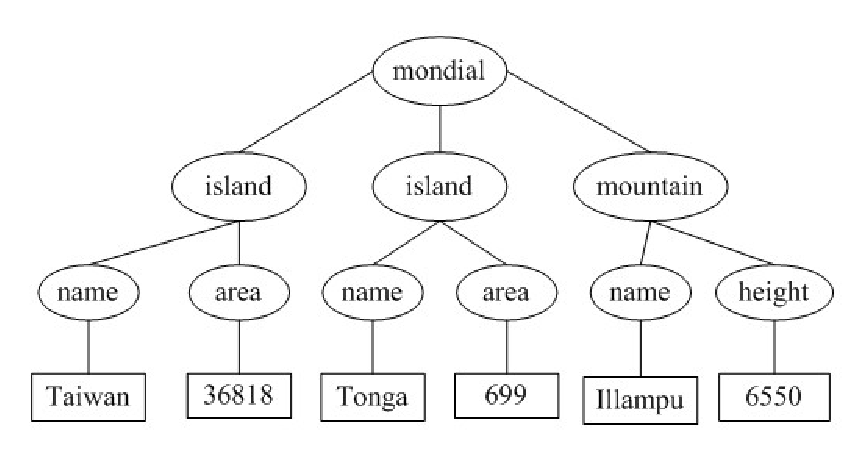
\includegraphics[width=0.4\textwidth]{XML}
\caption{树状结构}\label{fig:xml}
\vspace{\baselineskip}
\end{figure}


其插入图片的代码及其说明如下。
\vspace{1em}\noindent\hrule
\begin{verbatim}
\begin{figure}[htbp]
\centering
\includegraphics[width=0.4\textwidth]{文件名(.eps)}
\caption{标题}\label{标签名(通常为 fig:labelname)}
\vspace{\baselineskip} %表示图与正文空一行
\end{figure}
\end{verbatim}

\noindent\hrule

\begin{verbatim}
figure环境的可选参数[htbp]表示浮动图形所放置的位置,h (here)表示当前位置,t (top)表示页芯顶部,b (bottom)表示页芯底部,p (page)表示单独一页。在Word等软件中,图片通常插入到当前位置,如果当前页的剩余空间不够,图片将被移动到下一页,当前页就会出现很大的空白,其人工调整工作非常不便。由LaTeX提供的浮动图片功能,总是会按h->t->b->p的次序处理选项中的字母,自动调整图片的位置,大大减轻了工作量。
\centering命令将后续内容转换成每行皆居中的格式。
"\includegraphics"的可选参数用来设置图片插入文中的水平宽度,一般表示为正文宽度(\textwidth)的倍数。
\caption命令可选参数“标签名”为英文形式,一般不以图片或表格的数字顺序作为标签,而应包含一定的图片或表格信息,以便于文中引用(若图片、表格、公式、章节和参考文献等在文中出现的先后顺序发生了变化,其标注序号及其文中引用序号也会跟着发生变化,这一点是Word等软件所不能做到的)。另外,图题或表题并不会因为分页而与图片或表格体分置于两页,章节等各级标题也不会置于某页的最底部,LaTeX系统会自动调整它们在正文中的位置,这也是Word等软件所无法匹敌的。
\vspace将产生一定高度的竖直空白,必选参数为负值表示将后续文字位置向上提升,参数值可自行调整。em为长度单位,相当于大写字母M的宽度。\vspace{\baselineskip} 表示图与正文空一行。
引用方法:“见图~\ref{fig:figname}”、“如图~\ref{fig:figname}~所示”等。
\end{verbatim}

\noindent\hrule\vspace{1em}

若需要将~2~张及以上的图片并排插入到一行中,则需要采用\verb|minipage|环境,如图~\ref{fig:dd}~和图~\ref{fig:ds}~所示。
\begin{figure}[htbp]
\centering
\begin{minipage}{0.4\textwidth}
\centering
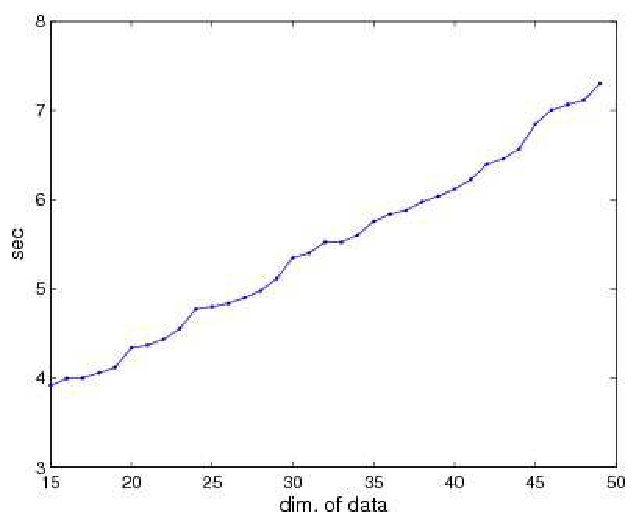
\includegraphics[width=\textwidth]{dataDimensions}
\caption{数据维数的变化}\label{fig:dd}
\end{minipage}
\begin{minipage}{0.4\textwidth}
\centering
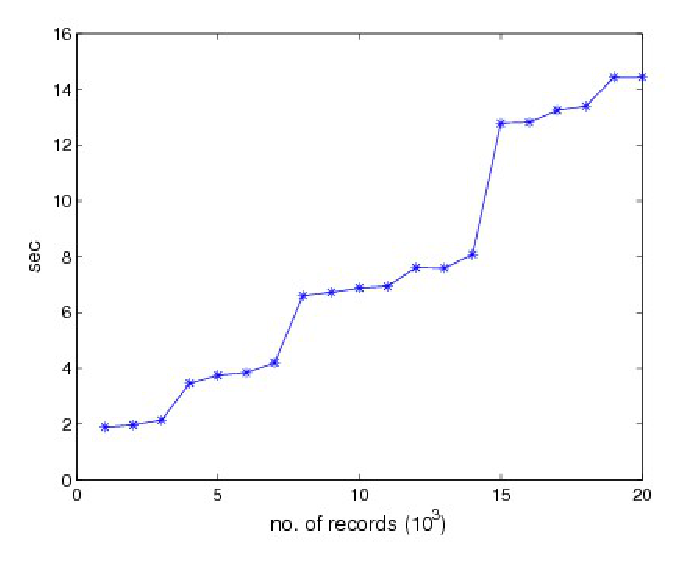
\includegraphics[width=\textwidth]{dataSize}
\caption{数据规模的变化}\label{fig:ds}
\end{minipage}
\vspace{\baselineskip}
\end{figure}

其代码如下所示。
\vspace{1em}\noindent\hrule
\begin{verbatim}
\begin{figure}[htbp]
\centering
\begin{minipage}{0.4\textwidth}
\centering
\includegraphics[width=\textwidth]{文件名}
\caption{标题}\label{fig:f1}
\end{minipage}
\begin{minipage}{0.4\textwidth}
\centering
\includegraphics[width=\textwidth]{文件名}
\caption{标题}\label{fig:f2}
\end{minipage}\vspace{\baselineskip}
\end{figure}
\end{verbatim}

\noindent\hrule

\begin{verbatim}
minipage环境的必选参数用来设置小页的宽度,若需要在一行中插入n个等宽图片,则每个小页的宽度应略小于(1/n)\textwidth。
\end{verbatim}

\noindent\hrule

\section{具有子图的图片插入方法}

图中若含有子图时,需要调用~subfigure~宏包, 如图~\ref{fig:subfig}~所示。
\begin{figure}[htbp]
  \centering
  \subfigure[Data Dimensions]{\label{fig:subfig:datadim}
                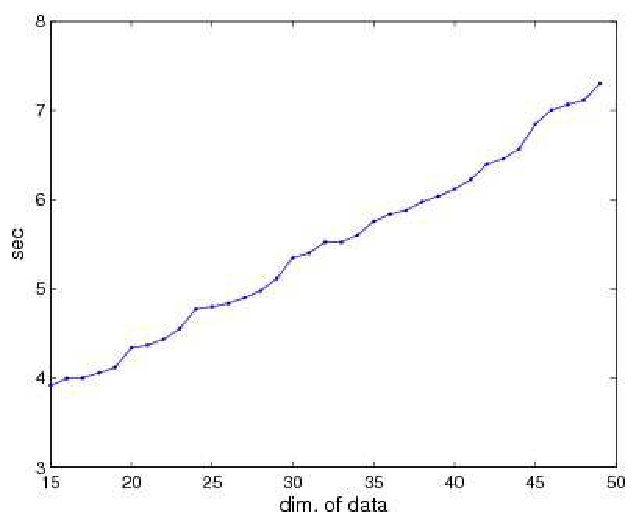
\includegraphics[width=0.4\textwidth]{dataDimensions}}
  \subfigure[Data Size]{\label{fig:subfig:datasize}
                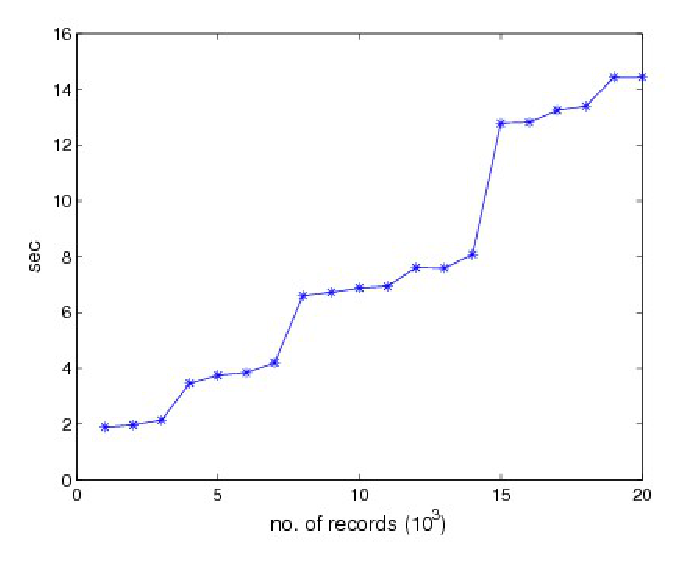
\includegraphics[width=0.4\textwidth]{dataSize}}
  \caption{Scalability of data}\label{fig:subfig}
\vspace{\baselineskip}
\end{figure}

其代码及其说明如下。
\vspace{1em}\noindent\hrule

\begin{verbatim}
\begin{figure}[htbp]
  \centering
  \subfigure[第1个子图标题]{
            \label{第1个子图标签(通常为 fig:subfig1:subsubfig1)}
            \includegraphics[width=0.4\textwidth]{文件名}}
  \subfigure[第2个子图标题]{
            \label{第2个子图标签(通常为 fig:subfig1:subsubfig2)}
            \includegraphics[width=0.4\textwidth]{文件名}}
  \caption{总标题}\label{总标签(通常为 fig:subfig1)}
\vspace{\baselineskip}
\end{figure}
\end{verbatim}

\noindent\hrule

\begin{verbatim}
子图的标签实际上可以随意设定,只要不重复就行。但为了更好的可读性,我们建议fig:subfig:subsubfig格式命名,这样我们从标签名就可以知道这是一个子图引用。
引用方法:总图的引用方法同本章第1节,子图的引用方法用\ref{fig:subfig:subsubfig}来代替。
\end{verbatim}

\noindent\hrule\vspace{1em}

子图的引用示例:如图~\ref{fig:subfig:datadim}~和图~\ref{fig:subfig:datasize}~所示。

若想获得插图方法的更多信息,参见网络上的~\href{ftp://ftp.tex.ac.uk/tex-archive/info/epslatex.pdf}{Using Imported Graphics in \LaTeX and pdf\LaTeX}~文档。 

\section{插入算法}

\begin{algorithm}[!h]
{
{
\renewcommand\baselinestretch{1.5}\selectfont %控制行距
\caption{ Scheduling Algorithm }
\label{alg:schedule}
\begin{algorithmic}[1]
\REQUIRE ~\\
A DFG $G=<V,E>$;\\
An allocation $A(G)$ for $G$.
\ENSURE ~\\
A schedule.
    \STATE{.......................}
    \FOR{$i\leftarrow\ 1\ to\ M$}    
        \STATE{.......................}
    \ENDFOR
    \STATE{.......................}
    \STATE{.......................}
    \STATE{.......................}
    \STATE{.......................}
    \STATE{.......................}
    \FOR{$k\leftarrow\ 1\ to\ |V|$}
        \STATE{.......................}
        \STATE{.......................}
        \STATE{.......................}
        \STATE{.......................}
    \IF{$LT_k==j$}
        \IF{there is no idle core in cluster $cl_{loc}$}
            \STATE{.......................}
            \STATE{.......................}
            \STATE{.......................}
            \STATE{.......................}
            \STATE{.......................}
            \STATE{.......................}
        \ELSE
            \STATE{.......................}
            \STATE{.......................}
            \STATE{.......................}
            \STATE{.......................}
            \STATE{.......................}
            \STATE{.......................}
        \ENDIF
    \ENDIF
    \ENDFOR
 

\end{algorithmic}
}
\par}
\end{algorithm}
%%% !Mode:: "TeX:UTF-8"

\chapter{表格的绘制方法}
\section{研究生毕业设计论文的绘表规范}

表应有自明性。表格不加左、右边线。表的编排建议采用国际通行的三线表。表内中文书写使用宋体五号字。

每个表格之上均应有表题(由表序和表名组成)。表序一般按章编排,如第~1~章第一个插表的序号为“表~1-1”等。表序与表名之间空两格,
表名使用中文五号字,居中。表名中不允许使用标点符号,表名后不加标点。
表头设计应简单明了,尽量不用斜线。表头中可采用化学,物理量等专业符号。

全表如用同一单位,则将单位符号移至表头右上角,加圆括号\cite{djy}。
表中数据应准确无误,书写清楚。数字空缺的格内加横线“-”(占~2~个数字宽度)。表内文字或数字上、下或左、右相同时,
采用通栏处理方式,不允许用“〃”、“同上”之类的写法。

表内文字使用宋体五号字,垂直居中书写,起行空一格、转行顶格、句末不加标点。
如某个表需要转页接排,在随后的各页上应重复表的编号。编号后加“(续表)”,表题可省略。续表应重复表头。
表格绘制完成之后,与正文空一行。

\section{普通表格的绘制方法}

表格应具有三线表格式,因此需要调用~booktabs~宏包,其标准格式如表~\ref{tab:table1}~所示。

\renewcommand\arraystretch{1.5}%控制行距
\begin{table}[!h]
\caption{基准测试集参数}\label{tab:bench}
\vspace{0.5em}
\centering
\begin{tabular}{l*{1}{C{2cm}}*{1}{L{6.2cm}}}
\toprule
Name         & $n$ & Description\\
\midrule
Random1      & 50  & Random graph generated by TGFF\\
Random2      & 100 & Random graph generated by TGFF\\
Random3      & 150 & Random graph generated by TGFF\\
Random4      & 200 & Random graph generated by TGFF\\
Random5      & 250 & Random graph generated by TGFF\\
Random6      & 300 & Random graph generated by TGFF\\
Random7      & 350 & Random graph generated by TGFF\\
Random8      & 400 & Random graph generated by TGFF\\
Random9      & 450 & Random graph generated by TGFF\\
Random10     & 500 & Random graph generated by TGFF\\
\bottomrule
\end{tabular}
\vspace{\baselineskip}
\end{table}
\renewcommand\arraystretch{1}

其绘制表格的代码及其说明如下。
\vspace{1em}\noindent\hrule

\begin{verbatim}
\begin{table}[htbp]
\caption{表标题}\label{标签名(通常为 tab:tablename)}
\vspace{0.5em}\centering\wuhao
\begin{tabular}{cc...c}
\toprule[1.5pt]
表头第1个格   & 表头第2个格   & ... & 表头第n个格  \\
\midrule[1pt]
表中数据(1,1) & 表中数据(1,2) & ... & 表中数据(1,n)\\
表中数据(2,1) & 表中数据(2,2) & ... & 表中数据(2,n)\\
表中数据(3,1) & 表中数据(3,2) & ... & 表中数据(3,n)\\
表中数据(4,1) & 表中数据(4,2) & ... & 表中数据(4,n)\\
...................................................\\
表中数据(m,1) & 表中数据(m,2) & ... & 表中数据(m,n)\\
\bottomrule[1.5pt]
\end{tabular}
\vspace{\baselineskip}
\end{table}
\end{verbatim}

\noindent\hrule

\begin{verbatim}
table环境是一个将表格嵌入文本的浮动环境。
\wuhao命令将表格的字号设置为五号字(10.5pt),在绘制表格结束退出时,不需要将字号再改回为\xiaosi,正文字号默认为小四号字(12pt)。
tabular环境的必选参数由每列对应一个格式字符所组成:c表示居中,l表示左对齐,r表示右对齐,其总个数应与表的列数相同。此外,@{文本}可以出现在任意两个上述的列格式之间,其中的文本将被插入每一行的同一位置。表格的各行以\\分隔,同一行的各列则以&分隔。
\toprule、\midrule和\bottomrule三个命令是由booktabs宏包提供的,其中\toprule和\bottomrule分别用来绘制表格的第一条(表格最顶部)和第三条(表格最底部)水平线,\midrule用来绘制第二条(表头之下)水平线,且第一条和第三条水平线的线宽为1.5pt,第二条水平线的线宽为1pt。
引用方法:“如表~\ref{tab:tablename}~所示”。
\end{verbatim}

\noindent\hrule

\section{长表格的绘制方法}

长表格是当表格在当前页排不下而需要转页接排的情况下所采用的一种表格环境。若长表格仍按照普通表格的绘制方法来获得,
其所使用的\verb|table|浮动环境无法实现表格的换页接排功能,表格下方过长部分会排在表格第1页的页脚以下。为了能够实现长表格的转页接排功能,
需要调用~longtable~宏包,由于长表格是跨页的文本内容,因此只需要单独的\verb|longtable|环境,所绘制的长表格的格式如表~\ref{tab:table2}~所示。

此长表格~\ref{tab:table2}~第~2~页的标题“编号(续表)”和表头是通过代码自动添加上去的,无需人工添加,若表格在页面中的竖直位置发生了变化,长表格在第~2~页
及之后各页的标题和表头位置能够始终处于各页的最顶部,也无需人工调整,\LaTeX~系统的这一优点是~Word~等软件所无法企及的。

下段内容是为了让下面的长表格分居两页,看到表标题“编号(续表)”的效果。摘录于《你若安好,便是晴天 -- 林徽因传》片段:

她叫林徽因,出生于杭州,是许多人梦中期待的白莲。她在雨雾之都伦敦,发生过一场空前绝后的康桥之恋。她爱过三个男子,爱得清醒,也爱得平静。徐志摩为她徜徉在康桥,深情地等待一场旧梦可以归来。梁思成与她携手走过千山万水,为完成使命而相约白头。金岳霖为她终身不娶,痴心不改地守候一世。可她懂得人生飘忽不定,要学会随遇而安。
真正的平静,不是避开车马喧嚣,而是在心中修篱种菊。尽管如流往事,每一天都涛声依旧,只要我们消除执念,便可寂静安然。愿每个人在纷呈世相中不会迷失荒径,可以端坐磐石上,醉倒落花前。
如果可以,请让我预支一段如莲的时光,哪怕将来某一天加倍偿还。这个雨季会在何时停歇,无从知晓。但我知道,你若安好,便是晴天。					 
\wuhao\begin{longtable}{ccc}
\caption{湖南大学各学院名称一览}\label{tab:table2}
 \vspace{0.5em}\\
\toprule[1.5pt] 学院名称 & 网址 & 联系电话  \\ \midrule[1pt]
\endfirsthead
\multicolumn{3}{c}{表~\thetable(续表)}\vspace{0.5em}\\
\toprule[1.5pt] 学院名称 & 网址 & 联系电话  \\ \midrule[1pt]
\endhead
\bottomrule[1.5pt]
\endfoot
机械工程学院& \url{http://tdjxxy.tju.edu.cn/}& 87401979\\
精密仪器与光电子工程学院&  \url{http://www2.tju.edu.cn/colleges/precision/cn/}& 27404775\\
电子信息工程学院& \url{http://www.tju.edu.cn/seie}& 27406956\\
电气与自动化工程学院& \url{http://www2.tju.edu.cn/colleges/automate/}& 27405477\\
建筑工程学院& \url{http://www2.tju.edu.cn/colleges/civil/}& 27404072\\
化工学院& \url{http://chemeng.tju.edu.cn/}& 27403389\\
材料科学与工程学院& \url{http://mse.tju.edu.cn}& 27406693 \\
建筑学院& \url{http://hgw022072.chinaw3.com/}& 27402724-2111\\
求是学部\\
管理与经济学部&	\url{ http://sm.tju.edu.cn}& 27403423\\
理学院& \url{ http://www.tju.edu.cn/science/}& 27404118\\
文法学院& \url{ http://www2.tju.edu.cn/colleges/sociology/new/}& 27403691\\
软件学院& \url{http://scs.tju.edu.cn}& 87401540\\
计算机科学与技术学院& \url{http://cs.tju.edu.cn/}& 27406538\\
马克思主义学院& \url{http://www2.tju.edu.cn/colleges/marxism/}& 27405348\\
环境科学与工程学院& \url{http://www.tju.edu.cn/see}& 87402072\\
药物科学与技术学院& \url{http://www2.tju.edu.cn/colleges/pharmtier/}& 87401830\\
教育学院& \url{http://soe.tju.edu.cn/}& 27401028\\
职业技术教育学院& \url{http://202.113.0.248:8888}\\
继续教育学院& \url{http://aectu.tju.edu.cn/}& 27406298\\
仁爱学院& \url{http://www.tjrac.edu.cn/}& 68579990\\
农业与生物工程学院& \url{http://202.113.13.169/site/nongxueyuan/}& 87402171\\
国际教育学院 & \url{http://www.ietju.com/}& 27406147\\
网络教育学院 & \url{http://www.etju.com/}& 27426952 \\

\end{longtable}\xiaosi
\vspace{\baselineskip}

绘制长表格的代码及其说明如下。
\vspace{1em}\noindent\hrule

\begin{verbatim}
\wuhao\begin{longtable}{cc...c}
\caption{表标题}\label{标签名(通常为 tab:tablename)}\\
\toprule[1.5pt] 表头第1个格 & 表头第2个格 & ... & 表头第n个格\\ \midrule[1pt]
\endfirsthead
\multicolumn{n}{c}{表~\thetable(续表)}\vspace{0.5em}\\
\toprule[1.5pt] 表头第1个格 & 表头第2个格 & ... & 表头第n个格\\ \midrule[1pt]
\endhead
\bottomrule[1.5pt]
\endfoot
表中数据(1,1) & 表中数据(1,2) & ... & 表中数据(1,n)\\
表中数据(2,1) & 表中数据(2,2) & ... & 表中数据(2,n)\\
...................................................\\
表中数据(m,1) & 表中数据(m,2) & ... & 表中数据(m,n)\\
\end{longtable}\xiaosi
\end{verbatim}

\noindent\hrule
\begin{verbatim}
在绘制长表格的前面留出一个空白行,并在第2行的一开始全局定义长表格的字号为五号字,这样能够保证长表格之前段落的行距保持不变。
在绘制长表格结束后,需要\xiaosi命令重新将字号改为小四号字。
\endhead之前的文字描述的是第2页及其之后各页的标题或表头;
\endfirsthead之前的文字描述的是第1页的标题和表头,若无此命令,则第1页的表头和标题由\endhead命令确定;
同理,\endfoot之前的文字描述的是除最后一页之外每页的表格底部内容;
\endlastfoot之前的文字描述的是最后一页的表格底部内容,若无此命令,
则最后一页的表格底部内容由\endfoot命令确定;由于规范中长表格每页底部内容均相同(水平粗线),因此模板中没有用到\endlastfoot命令。
\end{verbatim}

\noindent\hrule
\section{列宽可调表格的绘制方法}
论文中能用到列宽可调表格的情况共有两种:一种是当插入的表格某一单元格内容过长以至于一行放不下的情况,
另一种是当对公式中首次出现的物理量符号进行注释的情况。这两种情况都需要调用~tabularx~宏包。下面将分别对这两种情况下可调表格的绘制方法进行阐述。
\subsection{表格内某单元格内容过长的情况}

首先给出这种情况下的一个例子如表~\ref{tab:table3}~所示。
\begin{table}[htbp]
\caption{最小的三个正整数的英文表示法}\label{tab:table3}
\vspace{0.5em}\wuhao
\begin{tabularx}{\textwidth}{llX}
\toprule[1.5pt]
Value & Name & Alternate names, and names for sets of the given size\\\midrule[1pt]
1 & One & ace, single, singleton, unary, unit, unity\\
2 & Two & binary, brace, couple, couplet, distich, deuce, double, doubleton, duad, duality, duet, duo, dyad, pair, snake eyes, span, twain, twosome, yoke\\
3 & Three & deuce-ace, leash, set, tercet, ternary, ternion, terzetto, threesome, tierce, trey, triad, trine, trinity, trio, triplet, troika, hat-trick\\\bottomrule[1.5pt]
\end{tabularx}
\vspace{\baselineskip}
\end{table}
绘制这种表格的代码及其说明如下。
\vspace{1em}\noindent\hrule
\begin{verbatim}
\begin{table}[htbp]
\caption{表标题}\label{标签名(通常为 tab:tablename)}
\vspace{0.5em}\wuhao
\begin{tabularx}{\textwidth}{l...X...l}
\toprule[1.5pt]
表头第1个格   & ... & 表头第X个格   & ... & 表头第n个格  \\
\midrule[1pt]
表中数据(1,1) & ... & 表中数据(1,X) & ... & 表中数据(1,n)\\
表中数据(2,1) & ... & 表中数据(2,X) & ... & 表中数据(2,n)\\
.........................................................\\
表中数据(m,1) & ... & 表中数据(m,X) & ... & 表中数据(m,n)\\
\bottomrule[1.5pt]
\end{tabularx}
\vspace{\baselineskip}
\end{table}
\end{verbatim}

\noindent\hrule
\begin{verbatim}
tabularx环境共有两个必选参数:第1个参数用来确定表格的总宽度,这里取为排版表格能达到的最大宽度——正文宽度\textwidth;第2个参数用来确定每列格式,其中标为X的项表示该列的宽度可调,其宽度值由表格总宽度确定。
标为X的列一般选为单元格内容过长而无法置于一行的列,这样使得该列内容能够根据表格总宽度自动分行。若列格式中存在不止一个X项,则这些标为X的列的列宽相同,因此,一般不将内容较短的列设为X。
标为X的列均为左对齐,因此其余列一般选为l(左对齐),这样可使得表格美观,但也可以选为c或r。
\end{verbatim}

\noindent\hrule
\subsection{对物理量符号进行注释的情况}
为使得对公式中物理量符号注释的转行与破折号“———”后第一个字对齐,此处最好采用表格环境。此表格无任何线条,左对齐,
且在破折号处对齐,一共有“式中”二字、物理量符号和注释三列,表格的总宽度可选为文本宽度,因此应该采用\verb|tabularx|环境。
由\verb|tabularx|环境生成的对公式中物理量符号进行注释的公式如式(\ref{eq:1})所示。
%\vspace*{10pt}

\begin{equation}\label{eq:1}
\ddot{\boldsymbol{\rho}}-\frac{\mu}{R_{t}^{3}}\left(3\mathbf{R_{t}}\frac{\mathbf{R_{t}\rho}}{R_{t}^{2}}-\boldsymbol{\rho}\right)=\mathbf{a}
\end{equation}

\begin{tabularx}{\textwidth}{@{}l@{\quad}r@{———}X@{}}
式中& $\bm{\rho}$ &追踪飞行器与目标飞行器之间的相对位置矢量;\\
&  $\bm{\ddot{\rho}}$&追踪飞行器与目标飞行器之间的相对加速度;\\
&  $\mathbf{a}$   &推力所产生的加速度;\\
&  $\mathbf{R_t}$ & 目标飞行器在惯性坐标系中的位置矢量;\\
&  $\omega_{t}$ & 目标飞行器的轨道角速度;\\
&  $\mathbf{g}$ & 重力加速度,$=\frac{\mu}{R_{t}^{3}}\left(
3\mathbf{R_{t}}\frac{\mathbf{R_{t}\rho}}{R_{t}^{2}}-\bm{\rho}\right)=\omega_{t}^{2}\frac{R_{t}}{p}\left(
3\mathbf{R_{t}}\frac{\mathbf{R_{t}\rho}}{R_{t}^{2}}-\bm{\rho}\right)$,这里~$p$~是目标飞行器的轨道半通径。
\end{tabularx}
\vspace{\wordsep}

其中生成注释部分的代码及其说明如下。

\vspace{1em}\noindent\hrule

\begin{verbatim}
\begin{tabularx}{\textwidth}{@{}l@{\quad}r@{— — —}X@{}}
式中 & symbol-1 & symbol-1的注释内容;\\
     & symbol-2 & symbol-2的注释内容;\\
     .............................;\\
     & symbol-m & symbol-m的注释内容。
\end{tabularx}\vspace{\wordsep}
\end{verbatim}

\noindent\hrule

\begin{verbatim}
tabularx环境的第1个参数选为正文宽度,第2个参数里面各个符号的意义为:
    第1个@{}表示在“式中”二字左侧不插入任何文本,“式中”二字能够在正文中左对齐,若无此项,则“式中”二字左侧会留出一定的空白;
    @{\quad}表示在“式中”和物理量符号间插入一个空铅宽度的空白;
    @{— — —}实现插入破折号的功能,它由三个1/2的中文破折号构成;
    第2个@{}表示在注释内容靠近正文右边界的地方能够实现右对齐。
\end{verbatim}

\noindent\hrule\vspace{1em}

由此方法生成的注释内容应紧邻待注释公式并置于其下方,因此不能将代码放入\verb|table|浮动环境中。但此方法不能实现自动转页接排,
可能会在当前页剩余空间不够时,全部移动到下一页而导致当前页出现很大空白。因此在需要转页处理时,还请您手动将需要转页的代码放入一个
新的\verb|tabularx|环境中,将原来的一个\verb|tabularx|环境拆分为两个\verb|tabularx|环境。

若想获得绘制表格的更多信息,参见网络上的~\href{http://www.tug.org/pracjourn/2007-1/mori/}{Tables in \LaTeXe: Packages and Methods}~文档。


%%% !Mode:: "TeX:UTF-8"

\chapter{数学公式的输入方法}
\section{研究生毕业设计论文的公式规范}

论文中的公式应另起行,原则上应居中书写,与周围文字留有足够的空间区分开。
若公式前有文字(如“解”、“假定”等),文字空两格写,公式仍居中写。公式末不加标点。

公式应标注序号,并将序号置于括号内。 公式序号按章编排,如第~1~章第一个公式序号为“(1-1)”。公式的序号右端对齐。

公式较长时最好在等号“=”处转行,如难实现,则可在~$+$、$-$、$\times$、$\div$~运算符号处转行,转行时运算符号仅书写于转行式前,不重复书写。

文中引用公式时,一般用“见式~(1-1)”或“由公式~(1-1)”。

公式中用斜线表示“除”的关系时应采用括号,以免含糊不清,如~$a/(b\cos x)$。通常“乘”的关系在前,如~$a\cos x/b$而不写成~$(a/b)\cos x$。

不能用文字形式表示等式,如:$\textnormal{刚度}=\frac{{\textnormal{受力}}}{{\textnormal{受力方向的位移}}}$。

对于数学公式的输入方法,网络上有一个比较全面权威的文档\textbf{~\href{http://tug.ctan.org/cgi-bin/ctanPackageInformation.py?id=voss-mathmode}{Math mode}}~请大家事先大概浏览一下。下面将对学位论文中主要用到的数学公式排版形式进行阐述。

\section{生成~\LaTeX~数学公式的两种方法}
对于先前没有接触过~\LaTeX~的人来说,编写~\LaTeX~数学公式是一件很繁琐的事,尤其是对复杂的数学公式来说,更可以说是一件难以完成的任务。
实际上,生成~\LaTeX~数学公式有两种较为简便的方法,一种是基于~MathType~数学公式编辑器的方法,另一种是基于~MATLAB~商业数学软件的方法,
下面将分别对这两种数学公式的生成方法作一下简单介绍。

\subsection{基于~MathType~软件的数学公式生成方法}
MathType~是一款功能强大的数学公式编辑器软件,能够用来在文本环境中插入~Windows OLE~图形格式的复杂数学公式,所以应用比较普遍。但此软件只有~30~天的试用期,之后若再继续使用则需要付费购买才行。网络上有很多破解版的~MathType~软件可供下载免费使用,
笔者推荐下载安装版本号在~6.5~之上的中文破解版。

在安装好~MathType~之后,若在输入窗口中编写数学公式,复制到剪贴板上的仍然是图形格式的对象。
若希望得到可插入到~\LaTeX~编辑器中的文本格式对象,则需要对~MathType~软件做一下简单的设置:在~MathType~最上排的按钮中依次选择“参数选项
$\to$转换”,在弹出的对话窗中选中“转换到其它语言(文字):”,在转换下拉框中选择“Tex~--~--~LaTeX 2.09 and later”,并将对话框最下方的两个复选框全部勾掉,点击确定,这样,再从输入窗口中复制出来的对象就是文本格式的了,就可以直接将其粘贴到~\LaTeX~
编辑器中了。按照这种方法生成的数学公式两端分别有标记\verb|\[|和标记\verb|\]|,在这两个标记之间才是真正的数学公式代码。

若希望从~MathType~输入窗口中复制出来的对象为图形格式,则只需再选中“公示对象(Windows OLE~图形)”即可。

\subsection{基于~MATLAB~软件的数学公式生成方法}

MATLAB~是矩阵实验室(Matrix Laboratory)的简称,是美国~MathWorks~公司出品的商业数学软件。它是当今科研领域最常用的应用软件之一,
具有强大的矩阵计算、符号运算和数据可视化功能,是一种简单易用、可扩展的系统开发环境和平台。

MATLAB~中提供了一个~latex~函数,它可将符号表达式转化为~\LaTeX~数学公式的形式。其语法形式为~latex(s),其中,~s~为符号表达式,
之后再将~latex~函数的运算结果直接粘贴到~\LaTeX~编辑器中。从~\LaTeX~数学公式中可以发现,其中可能包含如下符号组合:

\begin{verbatim*}
\qquad=两个空铅(quad)宽度
\quad=一个空铅宽度
\;=5/18空铅宽度
\:=4/18空铅宽度
\,=3/18空铅宽度
\!=-3/18空铅宽度
\ =一个空格
\end{verbatim*}

所以最好将上述符号组合从数学公式中删除,从而使数学公式显得匀称美观。

对于~Word~等软件的使用者来说,在我们通过~MATLAB~运算得到符号表达式形式的运算结果时,在~Word~中插入运算结果需要借助于~MathType~软件,
通过在~MathType~中输入和~MATLAB~运算结果相对应的数学表达形式,之后再将~MathType~数学表达式转换为图形格式粘贴到~Word~中。实际上,
也可以将~MATLAB~中采用~latex~函数运行的结果直接粘贴到~MathType~中,再继续上述步骤,这样可以大大节省输入公式所需要的时间。
此方法在~MathType~6.5c~上验证通过,若您粘入到~MathType~中的仍然为从~MATLAB~中导入的代码,请您更新~MathType~软件。

\section{数学字体}
在数学模式下,常用的数学字体命令有如下几种:

\begin{verbatim}
\mathnormal或无命令 用数学字体打印文本;
\mathit             用斜体(\itshape)打印文本;
\mathbf             用粗体(\bfseries)打印文本;
\mathrm             用罗马体(\rmfamily)打印文本;
\mathsf             用无衬线字体(\sffamily)打印文本;
\mathtt             用打印机字体(\ttfamily)打印文本;
\mathcal            用书写体打印文本;
\end{verbatim}

在学位论文撰写中,只需要用到上面提到的~\verb|\mathit|、\verb|\mathbf|~和~\verb|\mathrm|~命令。若要得到~Times New Roman~的数学字体,则需要调用~txfonts~宏包(此宏包实际上采用的是~Nimbus Roman No9 L~字体,
它是开源系统中使用的免费字体,其字符字体与~Times New Roman~字体几乎完全相同);若要得到粗体数学字体,则需要调用~bm~宏包。表~\ref{tab:fonts}~中分别列出了得到阿拉伯数字、拉丁字母和希腊字母
各种数学字体的命令。

\begin{table}[htbp]
\caption{常用数学字体命令一览}\label{tab:fonts}
\vspace{0.5em}\centering\wuhao
\begin{tabular}{llll}
\toprule
 & 阿拉伯数字\&大写希腊字母 & 大小写拉丁字母 & 小写希腊字母  \\
\midrule
斜体 & \verb|\mathit{}| & \verb|无命令| & \verb|无命令|\\
粗斜体 & \verb|\bm{\mathit{}}| & \verb|\bm{}| & \verb|\bm{}|\\
直立体 & \verb|无命令| & \verb|\mathrm{}| & \verb|字母后加up|\\
粗体 & \verb|\mathbf{}或\bm{}| & \verb|\mathbf{}| & \verb|\bm{字母后加up}|\\
\bottomrule
\end{tabular}
\vspace{\baselineskip}
\end{table}

\noindent 下面列出了一些应采用直立数学字体的数学常数和数学符号。

\vspace{-0.5em}\begin{center}\begin{tabularx}{0.7\textwidth}{XX}
$\mathrm{d}$、 $\mathrm{D}$、 $\mathrm{p}$~———微分算子 & $\mathrm{e}$~———自然对数之底数\\
$\mathrm{i}$、 $\mathrm{j}$~———虚数单位 & $\piup$———圆周率\\
\end{tabularx}\end{center}

\section{行内公式}
出现在正文一行之内的公式称为行内公式,例如~$f(x)=\int_{a}^{b}\frac{\sin{x}}{x}\mathrm{d}x$。对于非矩阵和非多行形式的行内公式,一般不会使得行距发生变化,而~Word~等软件却会根据行内公式的竖直距离而自动调节行距,如图~\ref{fig:hangju}~所示。

\begin{figure}[htbp]
\centering
\subfigure[由~\LaTeX~系统生成的行内公式]{\label{fig:subfig:latex}
                \fbox{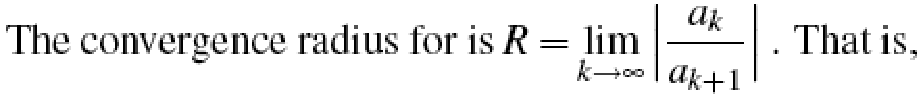
\includegraphics[width=0.55\textwidth]{latex}}}
\subfigure[由~Word软件生成的~.doc~格式行内公式]{\label{fig:subfig:word}
                \fbox{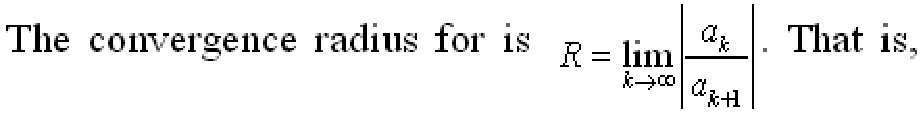
\includegraphics[width=0.55\textwidth]{word}}}
\subfigure[由~Word软件生成的~.pdf~格式行内公式]{\label{fig:subfig:pdf}
                \fbox{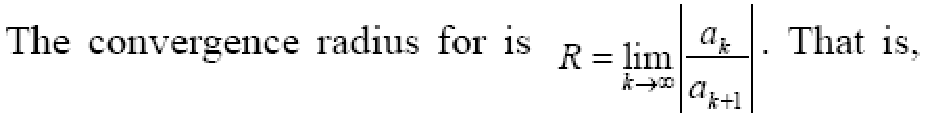
\includegraphics[width=0.55\textwidth]{pdf}}}

\caption{由~\LaTeX~和~Word~生成的~3~种行内公式屏显效果}\label{fig:hangju}
\vspace{-1em}
\end{figure}

这三幅图分别为~\LaTeX~和~Word~生成的行内公式屏显效果,从图中可看出,在~\LaTeX~文本含有公式的行内,在正文与公式之间对接工整,行距不变;而在~Word~文本含有公式的行内,在正文与公式之间对接不齐,行距变大。因此从这一点来说,
\LaTeX~系统在数学公式的排版上具有很大优势。

\LaTeX~提供的行内公式最简单、最有效的方法是采用~\TeX~本来的标记———开始和结束标记都写作~\$,例如本段开始的例子可由下面的输入得到。
\verb|$f(x)=\int_{a}^{b}\frac{\sin{x}}{x}\mathrm{d}x$|

\section{行间公式}
位于两行之间的公式称为行间公式,每个公式都是一个单独的段落,例如
\[\int_a^b{f\left(x\right)\mathrm{d}x}=\lim_{\left\|\Delta{x_i}\right\|\to 0}\sum_i{f\left(\xi_i\right)\Delta{x_i}}\]
除人工编号外,\LaTeX~各种类型行间公式的标记见表~\ref{tab:eqtag}。
\begin{table}[htbp]
\caption{各种类型行间公式的标记}\label{tab:eqtag}
\vspace{0.5em}\centering\wuhao
\begin{tabularx}{\textwidth}{cll}
\toprule
& 无编号 & 自动编号\\
\midrule
单行公式& \verb|\begin{displaymath}... \end{displaymath}|& \verb|\begin{equation}... \end{equation}|\\
        & 或~\verb|\[...\]| & \\
多行公式& \verb|\begin{eqnarray*}... \end{eqnarray*}|& \verb|\begin{eqnarray}... \end{eqnarray}|\\
\bottomrule
\end{tabularx}
\end{table}

另外,在自动编号的某行公式行尾添加标签~\verb|\nonumber|,可将该行转换为无编号形式。

行间多行公式需采用~\verb|eqnarray|~或~\verb|eqnarray*|~环境,它默认是一个列格式为~\verb|rcl|~的~3~列矩阵,并且中间列的字号要小一些,因此通常只将需要对齐的运算符号(通常为等号“=”)置于中间列。

\section{可自动调整大小的定界符}
若在左右两个定界符之前分别添加命令~\verb|\left|~和~\verb|\right|,则定界符可根据所包围公式大小自动调整其尺寸,这可从式(\ref{nodelimiter})和式(\ref{delimiter})中看出。
\begin{equation}\label{nodelimiter}
(\sum_{k=\frac12}^{N^2})
\end{equation}
\begin{equation}\label{delimiter}
\left(\sum_{k=\frac12}^{N^2}\right)
\end{equation}
式(\ref{nodelimiter})和式(\ref{delimiter})是在~\LaTeX~中分别输入如下代码得到的。
\begin{verbatim}
(\sum_{k=\frac12}^{N^2})
\left(\sum_{k=\frac12}^{N^2}\right)
\end{verbatim}
\verb|\left|~和~\verb|\right|~总是成对出现的,若只需在公式一侧有可自动调整大小的定界符,则只要用“.”代替另一侧那个无需打印出来的定界符即可。

若想获得关于此部分内容的更多信息,可参见~\href{http://tug.ctan.org/cgi-bin/ctanPackageInformation.py?id=voss-mathmode}{Math mode}~文档的第~8~章“Brackets, braces and parentheses”。

\section{数学重音符号}
数学重音符号通常用来区分同一字母表示的不同变量,输入方法如下(需要调用~\verb|amsmath|~宏包):

\vspace{0.5em}\noindent\wuhao\begin{tabularx}{\textwidth}{Xc|Xc|Xc}
 \verb|\acute| & $\acute{a}$ & \verb|\mathring| & $\mathring{a}$ & \verb|\underbrace| & $\underbrace{a}$ \\
 \verb|\bar| & $\bar{a}$ & \verb|\overbrace| & $\overbrace{a}$ & \verb|\underleftarrow| & $\underleftarrow{a}$ \\
 \verb|\breve| & $\breve{a}$ & \verb|\overleftarrow| & $\overleftarrow{a}$ & \verb|\underleftrightarrow| & $\underleftrightarrow{a}$ \\
 \verb|\check| & $\check{a}$ & \verb|\overleftrightarrow| & $\overleftrightarrow{a}$ & \verb|\underline| & $\underline{a}$ \\
 \verb|\dddot| & $\dddot{a}$ & \verb|\overline| & $\overline{a}$ & \verb|\underrightarrow| & $\underrightarrow{a}$ \\
 \verb|\ddot| & $\ddot{a}$ & \verb|\overrightarrow| & $\overrightarrow{a}$ & \verb|\vec| & $\vec{a}$ \\
 \verb|\dot| & $\dot{a}$ & \verb|\tilde| & $\tilde{a}$ & \verb|\widehat| & $\widehat{a}$ \\
 \verb|\grave| & $\grave{a}$ & \verb|\underbar| & $\underbar{a}$ & \verb|\widetilde| & $\widetilde{a}$ \\
 \verb|\hat| & $\hat{a}$
\end{tabularx}\vspace{0.5em}
\xiaosi 当需要在字母~$i$~和~$j$~的上方添加重音符号时,为了去掉这两个字母顶上的小点,这两个字母应该分别改用~\verb|\imath|~和~\verb|\jmath|。

如果遇到某些符号不知道该采用什么命令能输出它时,则可通过~\href{http://detexify.kirelabs.org/classify.html}{Detexify$^2$~网站}来获取符号命令。若用鼠标左键在此网页的方框区域内画出你所要找的符号形状,则会在网页右方列出和你所画符号形状相近的~5~个符号及其相对应的~\LaTeX~输入命令。若所列出的符号中不包括你所要找的符号,还可通过点击“Select from the complete list!”的链接以得分从低到高的顺序列出所有符号及其相对应的~\LaTeX~输入命令。

最后,建议大家还以~\href{http://tug.ctan.org/cgi-bin/ctanPackageInformation.py?id=voss-mathmode}{Math mode}~这篇~pdf~文档作为主要参考。若要获得最为标准、美观的数学公式排版形式,可以查查文档中是否有和你所要的排版形式相同或相近的代码段,通过修改代码段以获得你所要的数学公式排版形式。


%%% !Mode:: "TeX:UTF-8"

\chapter{罗列和定理环境使用方法}

\section{单层罗列环境}
湖南大学学位论文一般可采用两种罗列环境:一种是并列条目有同样标签的~\verb|itemize|~罗列环境,另一种是具有自动排序编号符号的~\verb|enumerate|~罗列环境。这两种罗列环境的样式参数可参考图~\ref{fig:list}。
\begin{figure}[htbp]
\centering
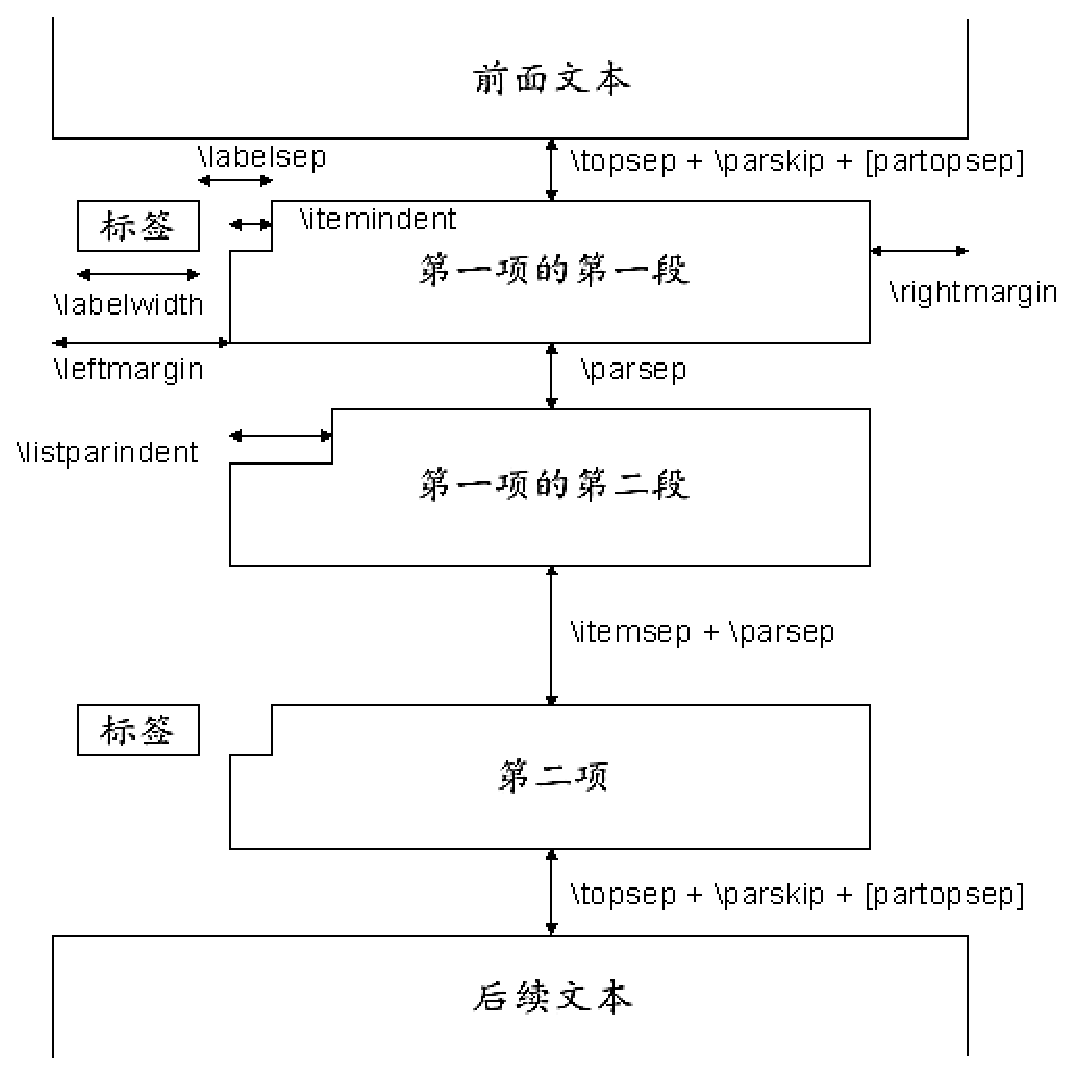
\includegraphics[width = 0.6\textwidth]{list}
\caption{罗列环境参数示意图}\label{fig:list}\vspace{-1em}
\end{figure}

通过调用~enumitem~宏包可以很方便地控制罗列环境的布局,其~format.tex~文件中的~\verb|\setitemize|~和~\verb|\setenumerate|~命令分别用来设置~\verb|itemize|~和~\verb|enumerate|~环境的样式参数。采用~\verb|itemize|~单层罗列环境的排版形式如下:

\begin{itemize}
\item 第一个条目文本内容
\item 第二个条目文本内容
\item 第三个条目文本内容
\end{itemize}

其代码如下

\begin{verbatim}
\begin{itemize}
  \item 第一个条目文本内容
  \item 第二个条目文本内容
  ...
  \item 第三个条目文本内容
\end{itemize}
\end{verbatim}

采用~\verb|enumerate|~单层罗列环境的排版形式如下:

\begin{enumerate}
\item 第一个条目文本内容
\item 第二个条目文本内容
\item 第三个条目文本内容
\end{enumerate}

其代码如下

\begin{verbatim}
\begin{enumerate}
  \item 第一个条目文本内容
  \item 第二个条目文本内容
  ...
  \item 第三个条目文本内容
\end{enumerate}
\end{verbatim}



\section{定理环境}

\begin{definition}[谱半径]\label{def:def1}
  称~$n$~阶方阵~$\mathbf{A}$~的全体特征值~$\lambda_1,\cdots,\lambda_n$~组成的集合为~$\mathbf{A}$~的谱,称
  $$\rho(\mathbf{A})=\max{\{|\lambda_1|,\cdots,|\lambda_n|\}}$$
\end{definition}
\begin{theorem}[相似充要条件]\label{lemma:l1}
  方阵$A$和$B$相似的充要条件是:~$A$~和~$B$~有全同的不变因子。
\end{theorem}
\begin{corollary}[推论1]\label{cor:cor1}
在赋范空间~$(X,\|\cdot\|)$~上定义~$d(x,y)=\|x-y\|$, 对任意~$x,y\in X$,~则~$(X,d)$~是距离空间。
\end{corollary}
\begin{proof}
  只需证明~$d(x,y)$~是距离。
\end{proof}
\newpage

定义代码如下:
\begin{verbatim}
 \begin{definition}[谱半径]\label{def:def1}
  称~$n$~阶方阵~$\mathbf{A}$~的全体特征值
  $\lambda_1,\cdots,\lambda_n$组成的集合为~$\mathbf{A}$~的谱,称
  $$\rho(\mathbf{A})=\max{\{|\lambda_1|,\cdots,|\lambda_n|\}}$$
\end{definition}
\end{verbatim}
\noindent\hrule

\vspace{0.1em}\noindent\hrule
\vspace{1em}
定理代码如下:
\begin{verbatim}
\begin{theorem}[相似充要条件]\label{lemma:l1}
  方阵$A$和$B$相似的充要条件是:$A$和$B$有全同的不变因子。
\end{theorem}
\end{verbatim}
\noindent\hrule\vspace{0.1em}

\noindent\hrule
\vspace{1em}
推论和证明代码如下:
\begin{verbatim}
\begin{corollary}[推论1]\label{cor:cor1}
在赋范空间~$(X,\|\cdot\|)$~上定义$d(x,y)=\|x-y\|$,
对任意$x,y\in X$,则$(X,d)$是距离空间。
\end{corollary}
\begin{proof}
  只需证明$d(x,y)$是距离。
\end{proof}
\end{verbatim}
\noindent\hrule\vspace{1em}

定理定义[]中是可选参数,用来说明定理的名称。其他环境格式书写与上面定理、定义、推论格式相同,可自己调用其他环境。
若需要书写定理定义等内容,而且带有顺序编号,需要采用如下环境。除了~\verb|proof|~环境之外,其余~9~个环境都可以有一个可选参数作为附加标题。

\begin{center}
\vspace{0.5em}\noindent\wuhao\begin{tabularx}{0.7\textwidth}{lX|lX}
定理 & \verb|theorem|~环境 & 定义 & \verb|definition|~环境 \\
例 & \verb|example|~环境 & 算法 & \verb|algorithm|~环境 \\
公理 & \verb|axiom|~环境 & 命题 & \verb|proposition|~环境 \\
引理 & \verb|lemma|~环境 & 推论 & \verb|corollary|~环境 \\
注解 & \verb|remark|~环境 & 证明 & \verb|proof|~环境 \\
\end{tabularx}
\end{center} 
%%% !Mode:: "TeX:UTF-8"

\addcontentsline{toc}{chapter}{结\quad 论} %添加到目录中
\chapter*{结\quad 论}

本文在分析分布式图处理系统和单机图处理系统的基础上,对目前图处理系统中的一些缺陷进行讨论,并在传统BSP计算模型的基础上,利用Actor并发模型对BSP模型进行优化,提出了基于Actor并发模型的BSP计算模型。通过对Actor-BSP模型的数据行为进行分析和讨论,将图数据分为两个部分:常驻内存的顶点状态信息和保存在磁盘上的边数据信息,同时利用内存映射优化IO操作。实验证明,GPSA图处理系统不仅能够在单机多核系统上高效的处理大规模图,同时还能够充分发挥多核的优势。本文的主要工作包括以下几个方面:

1、本论文在做了大量调研的基础上,对目前大规模图处理系统进行分析和对比,详细讨论目前存在于分布式图处理系统的困难问题,说明在单机系统上进行大规模图处理的可行性,对单机系统上的图处理系统进行分析和对比,从计算模型的角度出发,对传统的BSP模型进行优化,提出崭新的Actor-BSP图计算模型。Actor-BSP模型中将传统以顶点为中心的模型中顺序执行的计算过程和分发过程分离解耦,同时使用Actor代替线程,并将计算过程和分发过程分布在不同的Actor上,提高任务并发量。同时,Actor-BSP简化了图计算的流程,由于淡化顶点作为整个计算的中心的概念,顶点之间消息的传递转换为Actor之间的消息分发,计算过程和分发过程之间通过消息建立联系,从而无需再计算中缓存大量的消息,节省大量的IO操作。另外,Actor-BSP模型缩短了单个任务的平均执行时间,提升计算效率。

2、在Actor-BSP模型的基础上对数据的访问行为进行分析和讨论,由于新模型消息发送的随机性,就无法避免计算Actor对顶点状态信息的随机访问,与其他单机系统尽力回避随机访问的做法不同,GPSA大胆的采用数据分离的方法,将图数据分为两个独立的部分:顶点的状态信息和图的结构信息。其中,顶点的状态信息按照顺序存储的方式利用内存映射技术将其映射到内存来支持随机访问,提升效率。而对于图的结构信息则保持于磁盘上,可以采用顺序访问的方式,进一步节省IO操作。


3.独立完成了本文所论述的GPSA系统的调研,方案设计,具体编码实现和测试工作。列举PageRank、连通分量以及广度优先搜索三个常见图应用在GPSA系统上的实现,并将之与其他单机图处理系统从效率和多核利用率两个方面进行对比和分析,结果表明,GPSA不仅具有高效能够充分发挥多核优势的特点,而且具有较好的伸缩性与容错性。

虽然GPSA从改进计算模型角度出发,并取得良好的效果,但是GPSA依然存在一些不足,有待进一步完善。

首先,GPSA不支持图结构改变的应用。GPSA将图分为两部分:顶点信息和边。其中,顶点常驻内存,支持随机访问和更新,但是边、边上的权重等信息保存在磁盘上,需要尽量避免随机读写。

其次,GPSA使用JAVA实现,在实现过程中为避免频繁的垃圾回收造成的性能影响,在消息的封装中使用基本类型,造成消息的生成仅仅支持数字类型,无法支持字符串或者对象等。

最后,GPSA的设计初衷是能够兼容分布式以BSP为计算模型的大规模图处理系统,但是由于时间、经济等方面条件限制,该部分猜想的验证无力完成,希望能在将来能继续进行并开展在分布式方向的扩展和实验。

\end{verbatim}
那么,编译的时候就只编译未加~\%~的一章,在这个例子中,即本章~intros。

理论上,并不一定要把每章放在不同的文件中。但是这种自顶向下,分章节写作、编译的方法有利于提高效率,大大减少~Debug~过程中的编译时间,同时减小风险。

\section{参考文献生成方法}

\LaTeX~具有插入参考文献的能力。Google Scholar~网站上存在兼容~BibTeX~的参考文献信息,通过以下几个步骤,可以轻松完成参考文献的生成。
\begin{itemize}
  \item 在\href{http://scholar.google.com/}{谷歌学术搜索}中,
        点击\href{http://scholar.google.com/scholar_preferences?hl=en&as_sdt=0,5}{学术搜索设置}。
  \item 页面打开之后,在\textbf{文献管理软件}选项中选择\textbf{显示导入~BibTeX~的链接},单击保存设置,退出。
  \item 在谷歌学术搜索中检索到文献后,在文献条目区域单击导入~BibTeX~选项,页面中出现文献的引用信息。
  \item 将文献引用信息的内容复制之后,添加到~references~文件夹下的~reference.bib~中。
\end{itemize}

\section{编译注意事项}
\begin{enumerate}
  \item 由于模板使用~UTF-8~编码,所以源文件应该保存成~UTF-8~格式,否则可能出现中文字符无法识别的错误。
  本模板中每一个~.tex~文件的文件的开头已经加上一行:\\
    \verb|% !Mode:: "TeX:UTF-8"|\\
     这样可以确保~.tex~文件默认使用~UTF-8~的格式打开。读者如果删去此行,很有可能会导致中文字符显示乱码。
     在~WinEdt~编辑器中可以使用以下两种方式保存成~UTF-8~格式:
      \begin{enumerate}
        \item 先建立~.tex~文件,另存为~.tex~文件时,选择用~UTF-8~格式保存。
        \item
            在~WinEdt~编辑器中,选择\\
            \mbox{~Document$\to$Document Settings$\to$Document Mode $\to$TeX:UTF-8} 同时在~WinEdt~最下面的状态栏中,可以看到该文档是~TeX~格式还是~TeX:UTF-8~格式。
            当文档为~TeX:UTF-8~格式时,状态栏一般显示:
            \makebox[\textwidth][l]{Wrap | Indent | INS | LINE |Spell | TeX:UTF-8 | -src~等。}
      \end{enumerate}
  \item 如果在pdf书签中,中文显示乱码的话,则注意以下说明:
    \begin{verbatim}
        \usepackage{CJKutf8}
        % 1. 如果使用CJKutf8
        %    Hyperref中应使用unicode参数
        % 2. 如果使用CJK
        %    Hyperref则使用CJKbookmarks参数
        %    可惜得到的PDF书签是乱码,建议弃用
        % 3. Unicode选项和CJKbookmarks不能同时使用
        \usepackage[
        %CJKbookmarks=true,
        unicode=true
        ]{hyperref}
     \end{verbatim}
 \item 建议采用以下两种编译方式:
  \begin{enumerate}
     \item latex + bibtex + latex + latex + dvi2pdf. 在这种编译情况下,对应的~hnumain.tex~文件的第一行是\verb|\def\usewhat{dvipdfmx}|~(缺省设置)。 此时,所有图片文件应该保存为~.eps~格式,如~figures~文件夹里~.eps~图片。
          如果您选择在命令行中操作,可以在编译的时候依次输入~latex hnumain, bibtex hnumain, latex hnumain, latex hnumain~和~dvipdfmx hnumain, 编译完成之后,需要手动打开~pdf~文件。
     \item pdflatex + pdflatex. 在这种编译情况下,对应的~hnumain.tex~文件的第一行应该改为\verb|\def\usewhat{pdflatex}|~。 此时, 编译不支持~.eps~图片格式,此时需要在命令行下使用~epstopdf~指令将~figures~文件夹下 的~.eps~文件转化成~.pdf~文件格式,命令行中操作格式为~epstopdf a.eps~。
          在命令行编译的时候,依次输入~pdflatex hnumain~和~pdflatex hnumain, 编译完成之后,需要手动打开~pdf~文件。
  \end{enumerate}
\end{enumerate}

\section{系统要求}
    CTEX 2.8, MiKTeX 2.8, TeX Live 2009~或以上版本。使用推荐的~WinEdt 6.0~编辑器,可以完成文件的编辑和编译工作。

\section{\TeX~简介}

以下内容是~milksea@bbs.ctex.org~撰写的关于~\TeX~的简单介绍,略有改动。
注意这不是一个入门教程,不讲~\TeX~系统的配置安装,也不讲具体的~\LaTeX~代码。
这里仅仅试图以一些只言片语来解释:
进入这个门槛之前新手应该知道的注意事项,以及遇到问题以后该去如何解决问题。

\subsection{什么是 \TeX/\LaTeX,我是否应该选择它~?}

\TeX~是最早由高德纳(Donald Knuth)教授创建的一门标记式宏语言,
用来排版科技文章,尤其擅长处理复杂的数学公式。\TeX~同时也是处理这一语言的排版软件。
\LaTeX~是 Leslie Lamport 在~\TeX~基础上按内容/格式分离和模块化等思想建立的一集~\TeX~上的格式。

\TeX~本身的领域是专业排版领域
但现在~TeX/LaTeX~也被广泛用于生成电子文档甚至幻灯片等,~\TeX~语言的数学部分
偶尔也在其他一些地方使用。但注意~\TeX~并不适用于文书处理(Microsoft Office 的领域,以前和现在都不是)。

选择使用~\TeX/\LaTeX~的理由包括:
\begin{itemize}
\item 免费软件;
\item 专业的排版效果;
\item 是事实上的专业数学排版标准;
\item 广泛的西文期刊接收甚或只接收 LaTeX 格式的投稿;
\item[] ……
\end{itemize}
不选择使用~\TeX/\LaTeX~的理由包括:
\begin{itemize}
\item 需要相当精力学习;
\item 图文混合排版能力不够强;
\item 仅在数学、物理、计算机等领域流行;
\item 中文期刊的支持较差;
\item[] ……
\end{itemize}

请尽量清醒看待网上经常见到的关于~\TeX~与其他软件的优劣比较和口水战。在选择使用或离开之前,请先考虑
\TeX~的应用领域,想想它是否适合你的需要。


\subsection{我该用什么编辑器~?}

编辑器功能有简有繁,特色不一,从简单的纯文本编辑器到繁复的 Emacs,因人而易。基本功能有语法高亮、方便编译预览就很好了,扩充功能和定制有无限的可能。初学者可以使用功能简单、使用方便的专用编辑器,如 ~TeXWorks、Kile、WinEdt~等,或者类似所见即所得功能的~LyX;熟悉的人可以使用定制性更强的~Notepad++、SciTE、Vim、Emacs ~等。这方面的介绍很多,一开始不妨多试几种,找到最适合自己的才是最好的。

另外提醒一句,编辑器只是工作的助手,不必把它看得太重。

\subsection{我应该看什么~\LaTeX~读物~?}

这不是一个容易回答的问题,因为有许多选择,也同样有许多不合适的选择。
这里只是选出一个比较好的答案。更多更详细的介绍可以在版面和网上寻找(注意时效)。

近两年~\TeX~的中文处理发展很快,目前没有哪本书在中文处理方面给出一个最新进展的合适综述,
因而下面的介绍也不主要考虑中文处理。

\begin{enumerate}

\item 我能阅读英文。
\begin{enumerate}
\item 迅速入门:ltxprimer.pdf (LaTeX Tutorials: A Primer, India TUG)
\item 系统学习:A Guide to LaTeX, 4th Edition, Addison-Wesley
               有机械工业出版社的影印版(《\LaTeX{}~实用教程》)
\item 深入学习:要读许多书和文档,TeXbook 是必读的
\item 细节学习:去读你使用的每一个宏包的说明文档
\item 专题学习:阅读讲数学公式、图形、表格、字体等的专题文档
\end{enumerate}

\item 我更愿意阅读中文。
\begin{enumerate}
\item 迅速入门:lnotes.pdf (LaTeX Notes, 1.20, Alpha Huang)
\item 系统学习:《\LaTeXe{}~科技排版指南》,邓建松(电子版)
      如果不好找,可以阅读《\LaTeXe~入门与提高》第二版,陈志杰等,或者 《\LaTeXe~完全学习手册》,胡伟
\item 深入学习:~TeXbook0.pdf~(特可爱原本,TeXbook 的中译,xianxian)
\item 具体问题释疑:~CTeX-FAQ.pdf~,\\
        吴凌云,~\url{http://www.ctex.org/CTeXFAQ}~
\end{enumerate}
\end{enumerate}

遇见问题和解决问题的过程可以快速提高自己的技能,建议此时:
\begin{itemize}
  \item 利用~Google~搜索。
  \item 清楚,扼要地提出你的问题。
\end{itemize}

\subsection{什么知识会过时~?什么不会~?}

\TeX~是排版语言,也是广泛使用的软件,并且不断在发展中;
因此,总有一些东西会很快过时。作为学习~\TeX~的人,
免不了要看各种各样的书籍、电子文档和网络论坛上的只言片语,
因此了解什么知识会迅速过时,什么知识不会是十分重要的。

最稳定的是关于~Primitive \TeX~和~Plain \TeX~的知识,也就是 Knuth
在他的《The TeXbook》中介绍的内容。因为~\TeX~
系统开发的初衷就是稳定性,要求今天的文档到很久以后仍可以得到完全相同的结果,
因此 Knuth 限定了他的~\TeX~语言和相关实现的命令、语法。这些内容许多年来就没有多少变化,
在未来的一些年里也不会有什么变化。
Primitive \TeX~和 Plain \TeX~的知识主要包括 \TeX~排版的基本算法和原理,
盒子的原理,底层的 \TeX~命令等。其中技巧性的东西大多在宏包设计中,
初学者一般不会接触到很多;而基本原理则是常常被提到的,
譬如,~\TeX~把一切排版内容作为盒子(box)处理。

相对稳定的是关于基本~\LaTeXe~
的知识,也包括围绕~\LaTeXe~的一些核心宏包的知识。~\LaTeXe~
是自~1993~年以来的一个稳定的~\LaTeX~版本,直到最近的一次修订
(2005 年)都没有大的变动。
\LaTeX~的下一个计划中的版本~\LaTeX 3~遥遥无期,在可预见的将来,~\LaTeXe~不会过时。
\LaTeXe~的知识是目前大部分~\LaTeX~书籍的主体内容。关于~\LaTeX~的标准文档类
~(article、report、book、letter、slide~等),关于基本数学公式的输入,
文档的章节层次,表格和矩阵,图表浮动体,LR 盒子与段落盒子……
这些~\LaTeX~的核心内容都是最常用的,相对稳定的。
与~\LaTeXe~相匹配的核心宏包,
如~graphics(x)、ifthen、fontenc、doc~等,也同样是相对稳定的。
还有一些被非常广泛应用的宏包,如~amsmath~系列,也可以看作是相对稳定的。

简单地说,关于基本~\TeX/\LaTeX~的语言,都是比较稳定的。与之对应,实现或者支持~\TeX/\LaTeX~语言的软件,
包括在~\TeX/\LaTeX~基础上建立的新的宏,都不大稳定。

容易过时的是关于第三方~\LaTeX~宏包的知识、第三方~\TeX~工具的知识,以及新兴~\TeX~相关软件的知识等。
~\TeX~和~\LaTeX~语言是追求稳定的;但无论是宏包还是工具,作为不断更新软件,它们是不稳定的。
容易过时的技术很多,而且现在广泛地出现在几乎所有~\LaTeX~文档之中,因此需要特别引起注意:
宏包的过时的原因可
网络论坛上的只言片语的因此了解什么知识会迅速过时的什么知识不会是十分重
网络论坛上的只言片语的因此了解什么知识会迅速过时的什么知识不会是十分重
网络论坛上的只言片语的因此了解什么知识会迅速过时的什么知识不会是十分重
网络论坛上的只言片语的因此了解什么知识会迅速过时的什么知识不会是十分重
网络论坛上的只言片语的因此了解什么知识会迅速过时的什么知识不会是十分重
网络论坛上的只言片语的因此了解什么知识会迅速过时的什么知识不会是十分重
网络论坛上的只言片语的因此了解什么知识会迅速过时的什么知识不会是十分重
网络论坛上的只言片语的因此了解什么知识会迅速过时的什么知识不会是十分重
网络论坛上的只言片语的因此了解什么知识会迅速过时的什么知识不会是十分重
网络论坛上的只言片语的因此了解什么知识会迅速过时的什么知识不会是十分重
网络论坛上的只言片语的因此了解什么知识会迅速过时的什么知识不会是十分重
网络论坛上的只言片语的因此了解什么知识会迅速过时的什么知识不会是十分重
网络论坛上的只言片语的因此了解什么知识会迅速过时的什么知识不会是十分重
网络论坛上的只言片语的因此了解什么知识会迅速过时的什么知识不会是十分重
网络论坛上的只言片语的因此了解什么知识会迅速过时的什么知识不会是十分重
网络论坛上的只言片语的因此了解什么知识会迅速过时的什么知识不会是十分重
网络论坛上的只言片语的因此了解什么知识会迅速过时的什么知识不会是十分重
网络论坛上的只言片语的因此了解什么知识会迅速过时的什么知识不会是十分重
网络论坛上的只言片语的因此了解什么知识会迅速过时的什么知识不会是十分重
网络论坛上的只言片语的因此了解什么知识会迅速过时的什么知识不会是十分重
网络论坛上的只言片语的因此了解什么知识会迅速过时的什么知识不会是十分重
网络论坛上的只言片语的因此了解什么知识会迅速过时的什么知识不会是十分重
网络论坛上的只言片语的因此了解什么知识会迅速过时的什么知识不会是十分重
网络论坛上的只言片语的因此了解什么知识会迅速过时的什么知识不会是十分重
网络论坛上的只言片语的因此了解什么知识会迅速过时的什么知识不会是十分重
网络论坛上的只言片语的因此了解什么知识会迅速过时的什么知识不会是十分重
网络论坛上的只言片语的因此了解什么知识会迅速过时的什么知识不会是十分重
网络论坛上的只言片语的因此了解什么知识会迅速过时的什么知识不会是十分重
网络论坛上的只言片语的因此了解什么知识会迅速过时的什么知识不会是十分重
网络论坛上的只言片语的因此了解什么知识会迅速过时的什么知识不会是十分重
网络论坛上的只言片语的因此了解什么知识会迅速过时的什么知识不会是十分重
网络论坛上的只言片语的因此了解什么知识会迅速过时的什么知识不会是十分重
网络论坛上的只言片语的因此了解什么知识会迅速过时的什么知识不会是十分重
网络论坛上的只言片语的因此了解什么知识会迅速过时的什么知识不会是十分重
网络论坛上的只言片语的因此了解什么知识会迅速过时的什么知识不会是十分重
网络论坛上的只言片语的因此了解什么知识会迅速过时的什么知识不会是十分重
网络论坛上的只言片语的因此了解什么知识会迅速过时的什么知识不会是十分重
能是宏包本身的升级换代带来了新功能或不兼容,
也可能是同一功能的更新更好的宏包代替了旧的宏包。前者的典型例子比如绘图宏包~PGF/TikZ~,
现在的~2.00~版功能十分强大,和旧的~1.1x~版相差很大,和更旧的~0.x~版本则几乎完全不同;后
者的典型例子比如~caption~宏包先是被更新的~caption2~宏包代替,后来~caption~宏包更新又使得
caption2 宏包完全过时。——安装更新的发行版可以避免使用过旧的宏包;
认真阅读宏包自带的文档而不是搜索得到的陈旧片断可以避免采用过时的代码。

工具过时的主要原因也是升级换代和被其他工具替换。前者的典型例子是编辑器
WinEdt~在~5.5~以后的版本支持~UTF-8~编码,而旧版本不支持;
后者的典型例子是中文字体安装工具从~GBKFonts~到~xGBKFonts~到~FontsGen~不断被取代。
图形插入是一个在~\TeX~实现、宏包与外围工具方面都更新很快的东西。
在过去,最常用的输出格式是~PS(PostScript)~格式,因此插入的图像以~EPS~为主流。
使用~Dvips~为主要输出工具,外围工具有~GhostScript、bmeps~等等,相关宏包有~graphics~等,
相关文档如《\LaTeXe{}~ 插图指南》。

但凡提及“~\LaTeX~只支持~EPS~图形”的,就是这个过时的时代的产物。事实上~\TeX/\LaTeX~
并不限定任何图形格式,只不过是当时的输出格式(PS)和工具(Dvips)对~EPS~情有独钟而已。
后来 PDF 格式成为主流。~pdf\TeX、DVIPDFM、DVIPDFMx、XeTeX~工具则主要支持~PDF、PNG、JPG~格式的图形,
涉及一系列工具如~ImageMagick、ebb~等。

值得特别提出注意的就是,中文处理也一起是更新迅速、容易过时的部分。
而且因为中文处理一直没有一个“官方”的“标准”做法,软件、工具、
文档以及网上纷繁的笔记也就显得相当混乱。从八十年代开始的~CCT~系统、
天元系统,到后来的~CJK~方式,到近来的~XeTeX~和~LuaTeX~ 方式,
中文处理的原理、软件、宏包、配置方式等都在不断变化中。

%\section{后期工作}
%下表记录了~HNUThesis~计划中未来应该逐步实现的功能和特性:
%\begin{enumerate}
%  \item 编写更为详细的~HNUThesis~的使用手册和~FAQ~用户指南
%  \item 加入对课程结课论文的支持
%  \item 加入对天津大学学生经常参加的各种限时完成重大赛事的论文模板的支持,如全国研究生数学建模竞赛,以节省排版时间
%  \item 加入对~pdf~书签中章节中文编号的支持,如: 第1章 XXX
%  \item 加入对附录~A~等格式的支持
%  \item Linux~平台迁移和测试
%\end{enumerate}

\section{免责声明}

本模板依据《湖南大学关于博士、硕士学位论文统一格式的规定》和《湖南大学硕士论文模版》编写,适用于所有博士生的学位论文编写。然而,作者不保证本模板完全符合学校要求,也不对由此带来的风险和损失承担任何责任。

% !Mode:: "TeX:UTF-8"

\chapter{图片的插入方法}

\section{研究生毕业论文的插图规范}

图应有自明性。插图应与文字紧密配合,文图相符,内容正确。选图要力求精练,插图、照片应完整清晰。图中文字和数字等字号用宋体五号字。

机械工程图:采用第一角投影法,严格按照~GB4457---GB131-83《机械制图》标准规定。

数据流程图、程序流程图、系统流程图等按~GB1526-89~标准规定。

电气图:图形符号、文字符号等应符合有关标准的规定。

流程图:必须采用结构化程序并正确运用流程框图。

对无规定符号的图形应采用该行业的常用画法。

坐标图的坐标线均用细实线,粗细不得超过图中曲线,有数字标注的坐标图,必须注明坐标单位。

照片图要求主题和主要显示部分的轮廓鲜明,便于制版。如用放大或缩小的复制品,必须清晰,反差适中。照片上应有表示目的物尺寸的标度。

引用文献图表必须标注出处。

\subsection{图题及图中说明}
每个图均应有图题(由图序和图名组成),图名在图序之后空两格排写。图序按章编排,如第~1~章第一个插图的图号为“图~1-1”等。
图题置于图下,要求中文用宋体五号字,位置居中。有图注或其它说明时应置于图题之上。引用图应注明出处,在图题右上角加引用文献号。
图中若有分图时,分图题置于分图之下或图题之下,分图号用~a)、b)等表示。

图中各部分说明应采用中文(引用的外文图除外)或数字项号,各项文字说明置于图题之上(有分图题者,置于分图题之上)。

\subsection{插图编排}
插图之前,文中必须有关于本插图的提示,如“见图~1-1”、“如图~1-1~所示”等。插图与其图题为一个整体,不得拆开排写于两页。
插图处的该页空白不够排写该图整体时,则可将其后文字部分提前排写,将图移到次页。

\section{\LaTeX~中推荐使用的图片格式}
在~\LaTeX~中应用最多的图片格式是~EPS(Encapsulated PostScript)格式,它是一种专用的打印机描述语言,常用于印刷或打印输出。
EPS~格式图片可通过多种方式生成,这里介绍一款功能强大的免费图片处理软件———\href{http://www.imagemagick.org/}{ImageMagick},
此软件可将其它格式图片转换为~EPS~格式图片,同时还可以锐化图片,使图片的局部清晰一些。

此软件对图片的格式转换操作都是在命令提示符(cmd.exe)中实现的,可以通过“开始$\to$运行$\to$输入~cmd$\to$回车”或
“开始$\to$程序$\to$附件$\to$命令提示符”找到它。在命令提示符下,首先采用“盘符命令”或“cd~命令”将当前目录改为待处理图片所在的目录,
在此目录下就可通过~convert~命令将图片转换为~EPS~格式,其命令的语法格式为

\indent\verb|convert [可选参数] 原文件名.原扩展名 新文件名.eps|.

若~convert~命令中无可选参数,则将原来的图片格式直接转换为~EPS~格式,对图片不进行任何处理,这也是最常用的方法。
也可以选用可选参数,可选参数有很多选择,但最常用的有如下两个:

\verb|-sharpen radius{xsigma}|———此参数用来锐化图片,一般用在图片像素不高,需要提高图片清晰度的情况下。其中~radius~只能为整数,
它用来确定转换命令采取哪一种锐化算法,我们可以只取~radius~为~0;sigma~为所采取算法的锐化度,它的取值为~$0.1 - 3$~之间的任意一个浮点数,
数值越大,锐化程度也越大,通常取为~$0.1 - 3$~之间;x~在参数中为分隔符。

\verb|-resize geometry|———此参数用来改变图片的大小,若图片的存储空间过大,可通过此命令缩小图片尺寸,但同时也将导致图片像素降低,
其具体用法请参见\href{http://www.imagemagick.org/script/command-line-options.php#resize}{-resize geometry~的官方说明}。

除此之外,一些文字处理软件和科学计算软件也支持生成~EPS~格式的文件,请使用“另存为”功能查看某款软件是否能够将图片以~EPS~格式的形式保存。

\section{单张图片的插入方法}
单张图片独自占一行的插入形式如图~\ref{fig:xml}~所示。
\begin{figure}[htbp]
\centering
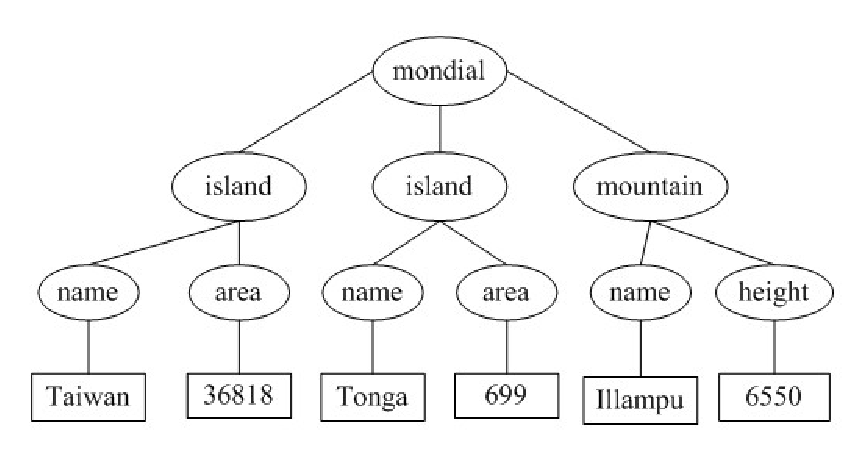
\includegraphics[width=0.4\textwidth]{XML}
\caption{树状结构}\label{fig:xml}
\vspace{\baselineskip}
\end{figure}


其插入图片的代码及其说明如下。
\vspace{1em}\noindent\hrule
\begin{verbatim}
\begin{figure}[htbp]
\centering
\includegraphics[width=0.4\textwidth]{文件名(.eps)}
\caption{标题}\label{标签名(通常为 fig:labelname)}
\vspace{\baselineskip} %表示图与正文空一行
\end{figure}
\end{verbatim}

\noindent\hrule

\begin{verbatim}
figure环境的可选参数[htbp]表示浮动图形所放置的位置,h (here)表示当前位置,t (top)表示页芯顶部,b (bottom)表示页芯底部,p (page)表示单独一页。在Word等软件中,图片通常插入到当前位置,如果当前页的剩余空间不够,图片将被移动到下一页,当前页就会出现很大的空白,其人工调整工作非常不便。由LaTeX提供的浮动图片功能,总是会按h->t->b->p的次序处理选项中的字母,自动调整图片的位置,大大减轻了工作量。
\centering命令将后续内容转换成每行皆居中的格式。
"\includegraphics"的可选参数用来设置图片插入文中的水平宽度,一般表示为正文宽度(\textwidth)的倍数。
\caption命令可选参数“标签名”为英文形式,一般不以图片或表格的数字顺序作为标签,而应包含一定的图片或表格信息,以便于文中引用(若图片、表格、公式、章节和参考文献等在文中出现的先后顺序发生了变化,其标注序号及其文中引用序号也会跟着发生变化,这一点是Word等软件所不能做到的)。另外,图题或表题并不会因为分页而与图片或表格体分置于两页,章节等各级标题也不会置于某页的最底部,LaTeX系统会自动调整它们在正文中的位置,这也是Word等软件所无法匹敌的。
\vspace将产生一定高度的竖直空白,必选参数为负值表示将后续文字位置向上提升,参数值可自行调整。em为长度单位,相当于大写字母M的宽度。\vspace{\baselineskip} 表示图与正文空一行。
引用方法:“见图~\ref{fig:figname}”、“如图~\ref{fig:figname}~所示”等。
\end{verbatim}

\noindent\hrule\vspace{1em}

若需要将~2~张及以上的图片并排插入到一行中,则需要采用\verb|minipage|环境,如图~\ref{fig:dd}~和图~\ref{fig:ds}~所示。
\begin{figure}[htbp]
\centering
\begin{minipage}{0.4\textwidth}
\centering
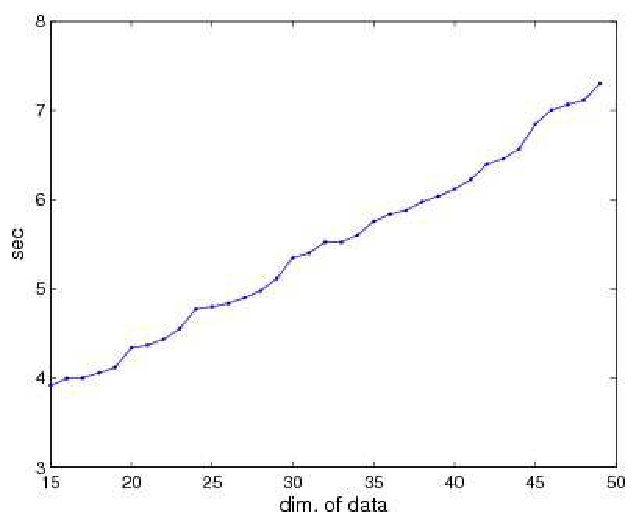
\includegraphics[width=\textwidth]{dataDimensions}
\caption{数据维数的变化}\label{fig:dd}
\end{minipage}
\begin{minipage}{0.4\textwidth}
\centering
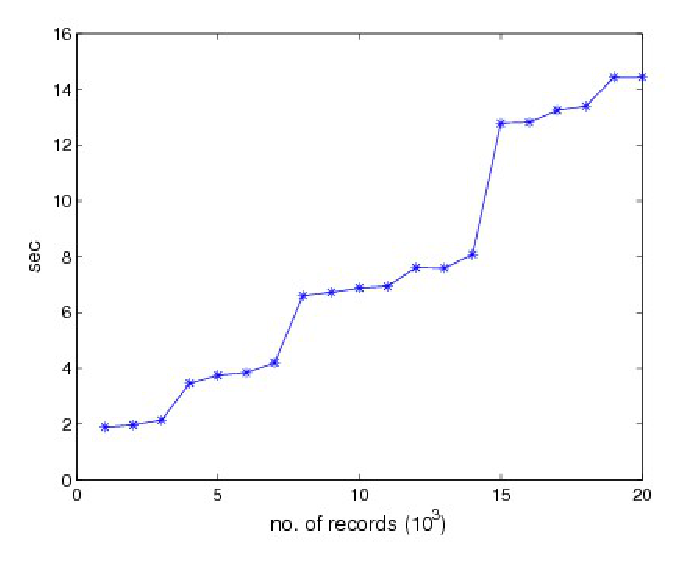
\includegraphics[width=\textwidth]{dataSize}
\caption{数据规模的变化}\label{fig:ds}
\end{minipage}
\vspace{\baselineskip}
\end{figure}

其代码如下所示。
\vspace{1em}\noindent\hrule
\begin{verbatim}
\begin{figure}[htbp]
\centering
\begin{minipage}{0.4\textwidth}
\centering
\includegraphics[width=\textwidth]{文件名}
\caption{标题}\label{fig:f1}
\end{minipage}
\begin{minipage}{0.4\textwidth}
\centering
\includegraphics[width=\textwidth]{文件名}
\caption{标题}\label{fig:f2}
\end{minipage}\vspace{\baselineskip}
\end{figure}
\end{verbatim}

\noindent\hrule

\begin{verbatim}
minipage环境的必选参数用来设置小页的宽度,若需要在一行中插入n个等宽图片,则每个小页的宽度应略小于(1/n)\textwidth。
\end{verbatim}

\noindent\hrule

\section{具有子图的图片插入方法}

图中若含有子图时,需要调用~subfigure~宏包, 如图~\ref{fig:subfig}~所示。
\begin{figure}[htbp]
  \centering
  \subfigure[Data Dimensions]{\label{fig:subfig:datadim}
                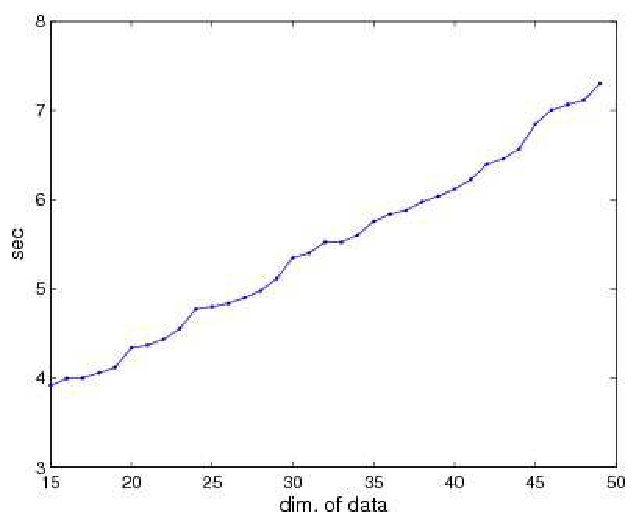
\includegraphics[width=0.4\textwidth]{dataDimensions}}
  \subfigure[Data Size]{\label{fig:subfig:datasize}
                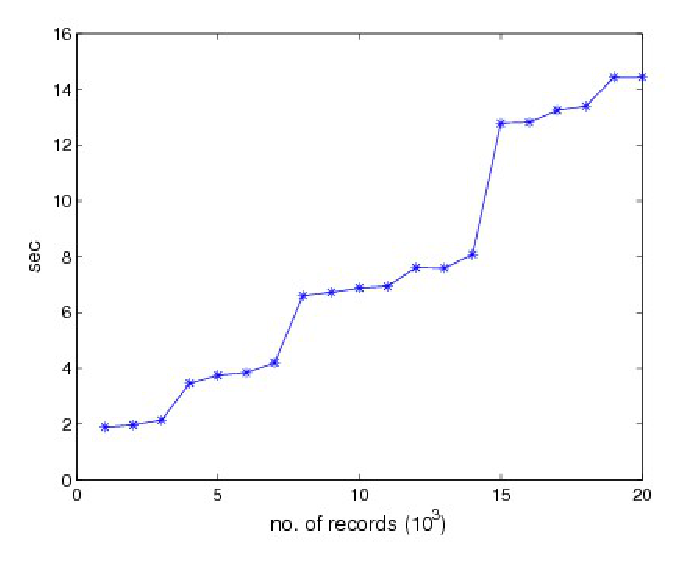
\includegraphics[width=0.4\textwidth]{dataSize}}
  \caption{Scalability of data}\label{fig:subfig}
\vspace{\baselineskip}
\end{figure}

其代码及其说明如下。
\vspace{1em}\noindent\hrule

\begin{verbatim}
\begin{figure}[htbp]
  \centering
  \subfigure[第1个子图标题]{
            \label{第1个子图标签(通常为 fig:subfig1:subsubfig1)}
            \includegraphics[width=0.4\textwidth]{文件名}}
  \subfigure[第2个子图标题]{
            \label{第2个子图标签(通常为 fig:subfig1:subsubfig2)}
            \includegraphics[width=0.4\textwidth]{文件名}}
  \caption{总标题}\label{总标签(通常为 fig:subfig1)}
\vspace{\baselineskip}
\end{figure}
\end{verbatim}

\noindent\hrule

\begin{verbatim}
子图的标签实际上可以随意设定,只要不重复就行。但为了更好的可读性,我们建议fig:subfig:subsubfig格式命名,这样我们从标签名就可以知道这是一个子图引用。
引用方法:总图的引用方法同本章第1节,子图的引用方法用\ref{fig:subfig:subsubfig}来代替。
\end{verbatim}

\noindent\hrule\vspace{1em}

子图的引用示例:如图~\ref{fig:subfig:datadim}~和图~\ref{fig:subfig:datasize}~所示。

若想获得插图方法的更多信息,参见网络上的~\href{ftp://ftp.tex.ac.uk/tex-archive/info/epslatex.pdf}{Using Imported Graphics in \LaTeX and pdf\LaTeX}~文档。 

\section{插入算法}

\begin{algorithm}[!h]
{
{
\renewcommand\baselinestretch{1.5}\selectfont %控制行距
\caption{ Scheduling Algorithm }
\label{alg:schedule}
\begin{algorithmic}[1]
\REQUIRE ~\\
A DFG $G=<V,E>$;\\
An allocation $A(G)$ for $G$.
\ENSURE ~\\
A schedule.
    \STATE{.......................}
    \FOR{$i\leftarrow\ 1\ to\ M$}    
        \STATE{.......................}
    \ENDFOR
    \STATE{.......................}
    \STATE{.......................}
    \STATE{.......................}
    \STATE{.......................}
    \STATE{.......................}
    \FOR{$k\leftarrow\ 1\ to\ |V|$}
        \STATE{.......................}
        \STATE{.......................}
        \STATE{.......................}
        \STATE{.......................}
    \IF{$LT_k==j$}
        \IF{there is no idle core in cluster $cl_{loc}$}
            \STATE{.......................}
            \STATE{.......................}
            \STATE{.......................}
            \STATE{.......................}
            \STATE{.......................}
            \STATE{.......................}
        \ELSE
            \STATE{.......................}
            \STATE{.......................}
            \STATE{.......................}
            \STATE{.......................}
            \STATE{.......................}
            \STATE{.......................}
        \ENDIF
    \ENDIF
    \ENDFOR
 

\end{algorithmic}
}
\par}
\end{algorithm}
% !Mode:: "TeX:UTF-8"

\chapter{表格的绘制方法}
\section{研究生毕业设计论文的绘表规范}

表应有自明性。表格不加左、右边线。表的编排建议采用国际通行的三线表。表内中文书写使用宋体五号字。

每个表格之上均应有表题(由表序和表名组成)。表序一般按章编排,如第~1~章第一个插表的序号为“表~1-1”等。表序与表名之间空两格,
表名使用中文五号字,居中。表名中不允许使用标点符号,表名后不加标点。
表头设计应简单明了,尽量不用斜线。表头中可采用化学,物理量等专业符号。

全表如用同一单位,则将单位符号移至表头右上角,加圆括号\cite{djy}。
表中数据应准确无误,书写清楚。数字空缺的格内加横线“-”(占~2~个数字宽度)。表内文字或数字上、下或左、右相同时,
采用通栏处理方式,不允许用“〃”、“同上”之类的写法。

表内文字使用宋体五号字,垂直居中书写,起行空一格、转行顶格、句末不加标点。
如某个表需要转页接排,在随后的各页上应重复表的编号。编号后加“(续表)”,表题可省略。续表应重复表头。
表格绘制完成之后,与正文空一行。

\section{普通表格的绘制方法}

表格应具有三线表格式,因此需要调用~booktabs~宏包,其标准格式如表~\ref{tab:table1}~所示。

\renewcommand\arraystretch{1.5}%控制行距
\begin{table}[!h]
\caption{基准测试集参数}\label{tab:bench}
\vspace{0.5em}
\centering
\begin{tabular}{l*{1}{C{2cm}}*{1}{L{6.2cm}}}
\toprule
Name         & $n$ & Description\\
\midrule
Random1      & 50  & Random graph generated by TGFF\\
Random2      & 100 & Random graph generated by TGFF\\
Random3      & 150 & Random graph generated by TGFF\\
Random4      & 200 & Random graph generated by TGFF\\
Random5      & 250 & Random graph generated by TGFF\\
Random6      & 300 & Random graph generated by TGFF\\
Random7      & 350 & Random graph generated by TGFF\\
Random8      & 400 & Random graph generated by TGFF\\
Random9      & 450 & Random graph generated by TGFF\\
Random10     & 500 & Random graph generated by TGFF\\
\bottomrule
\end{tabular}
\vspace{\baselineskip}
\end{table}
\renewcommand\arraystretch{1}

其绘制表格的代码及其说明如下。
\vspace{1em}\noindent\hrule

\begin{verbatim}
\begin{table}[htbp]
\caption{表标题}\label{标签名(通常为 tab:tablename)}
\vspace{0.5em}\centering\wuhao
\begin{tabular}{cc...c}
\toprule[1.5pt]
表头第1个格   & 表头第2个格   & ... & 表头第n个格  \\
\midrule[1pt]
表中数据(1,1) & 表中数据(1,2) & ... & 表中数据(1,n)\\
表中数据(2,1) & 表中数据(2,2) & ... & 表中数据(2,n)\\
表中数据(3,1) & 表中数据(3,2) & ... & 表中数据(3,n)\\
表中数据(4,1) & 表中数据(4,2) & ... & 表中数据(4,n)\\
...................................................\\
表中数据(m,1) & 表中数据(m,2) & ... & 表中数据(m,n)\\
\bottomrule[1.5pt]
\end{tabular}
\vspace{\baselineskip}
\end{table}
\end{verbatim}

\noindent\hrule

\begin{verbatim}
table环境是一个将表格嵌入文本的浮动环境。
\wuhao命令将表格的字号设置为五号字(10.5pt),在绘制表格结束退出时,不需要将字号再改回为\xiaosi,正文字号默认为小四号字(12pt)。
tabular环境的必选参数由每列对应一个格式字符所组成:c表示居中,l表示左对齐,r表示右对齐,其总个数应与表的列数相同。此外,@{文本}可以出现在任意两个上述的列格式之间,其中的文本将被插入每一行的同一位置。表格的各行以\\分隔,同一行的各列则以&分隔。
\toprule、\midrule和\bottomrule三个命令是由booktabs宏包提供的,其中\toprule和\bottomrule分别用来绘制表格的第一条(表格最顶部)和第三条(表格最底部)水平线,\midrule用来绘制第二条(表头之下)水平线,且第一条和第三条水平线的线宽为1.5pt,第二条水平线的线宽为1pt。
引用方法:“如表~\ref{tab:tablename}~所示”。
\end{verbatim}

\noindent\hrule

\section{长表格的绘制方法}

长表格是当表格在当前页排不下而需要转页接排的情况下所采用的一种表格环境。若长表格仍按照普通表格的绘制方法来获得,
其所使用的\verb|table|浮动环境无法实现表格的换页接排功能,表格下方过长部分会排在表格第1页的页脚以下。为了能够实现长表格的转页接排功能,
需要调用~longtable~宏包,由于长表格是跨页的文本内容,因此只需要单独的\verb|longtable|环境,所绘制的长表格的格式如表~\ref{tab:table2}~所示。

此长表格~\ref{tab:table2}~第~2~页的标题“编号(续表)”和表头是通过代码自动添加上去的,无需人工添加,若表格在页面中的竖直位置发生了变化,长表格在第~2~页
及之后各页的标题和表头位置能够始终处于各页的最顶部,也无需人工调整,\LaTeX~系统的这一优点是~Word~等软件所无法企及的。

下段内容是为了让下面的长表格分居两页,看到表标题“编号(续表)”的效果。摘录于《你若安好,便是晴天 -- 林徽因传》片段:

她叫林徽因,出生于杭州,是许多人梦中期待的白莲。她在雨雾之都伦敦,发生过一场空前绝后的康桥之恋。她爱过三个男子,爱得清醒,也爱得平静。徐志摩为她徜徉在康桥,深情地等待一场旧梦可以归来。梁思成与她携手走过千山万水,为完成使命而相约白头。金岳霖为她终身不娶,痴心不改地守候一世。可她懂得人生飘忽不定,要学会随遇而安。
真正的平静,不是避开车马喧嚣,而是在心中修篱种菊。尽管如流往事,每一天都涛声依旧,只要我们消除执念,便可寂静安然。愿每个人在纷呈世相中不会迷失荒径,可以端坐磐石上,醉倒落花前。
如果可以,请让我预支一段如莲的时光,哪怕将来某一天加倍偿还。这个雨季会在何时停歇,无从知晓。但我知道,你若安好,便是晴天。					 
\wuhao\begin{longtable}{ccc}
\caption{湖南大学各学院名称一览}\label{tab:table2}
 \vspace{0.5em}\\
\toprule[1.5pt] 学院名称 & 网址 & 联系电话  \\ \midrule[1pt]
\endfirsthead
\multicolumn{3}{c}{表~\thetable(续表)}\vspace{0.5em}\\
\toprule[1.5pt] 学院名称 & 网址 & 联系电话  \\ \midrule[1pt]
\endhead
\bottomrule[1.5pt]
\endfoot
机械工程学院& \url{http://tdjxxy.tju.edu.cn/}& 87401979\\
精密仪器与光电子工程学院&  \url{http://www2.tju.edu.cn/colleges/precision/cn/}& 27404775\\
电子信息工程学院& \url{http://www.tju.edu.cn/seie}& 27406956\\
电气与自动化工程学院& \url{http://www2.tju.edu.cn/colleges/automate/}& 27405477\\
建筑工程学院& \url{http://www2.tju.edu.cn/colleges/civil/}& 27404072\\
化工学院& \url{http://chemeng.tju.edu.cn/}& 27403389\\
材料科学与工程学院& \url{http://mse.tju.edu.cn}& 27406693 \\
建筑学院& \url{http://hgw022072.chinaw3.com/}& 27402724-2111\\
求是学部\\
管理与经济学部&	\url{ http://sm.tju.edu.cn}& 27403423\\
理学院& \url{ http://www.tju.edu.cn/science/}& 27404118\\
文法学院& \url{ http://www2.tju.edu.cn/colleges/sociology/new/}& 27403691\\
软件学院& \url{http://scs.tju.edu.cn}& 87401540\\
计算机科学与技术学院& \url{http://cs.tju.edu.cn/}& 27406538\\
马克思主义学院& \url{http://www2.tju.edu.cn/colleges/marxism/}& 27405348\\
环境科学与工程学院& \url{http://www.tju.edu.cn/see}& 87402072\\
药物科学与技术学院& \url{http://www2.tju.edu.cn/colleges/pharmtier/}& 87401830\\
教育学院& \url{http://soe.tju.edu.cn/}& 27401028\\
职业技术教育学院& \url{http://202.113.0.248:8888}\\
继续教育学院& \url{http://aectu.tju.edu.cn/}& 27406298\\
仁爱学院& \url{http://www.tjrac.edu.cn/}& 68579990\\
农业与生物工程学院& \url{http://202.113.13.169/site/nongxueyuan/}& 87402171\\
国际教育学院 & \url{http://www.ietju.com/}& 27406147\\
网络教育学院 & \url{http://www.etju.com/}& 27426952 \\

\end{longtable}\xiaosi
\vspace{\baselineskip}

绘制长表格的代码及其说明如下。
\vspace{1em}\noindent\hrule

\begin{verbatim}
\wuhao\begin{longtable}{cc...c}
\caption{表标题}\label{标签名(通常为 tab:tablename)}\\
\toprule[1.5pt] 表头第1个格 & 表头第2个格 & ... & 表头第n个格\\ \midrule[1pt]
\endfirsthead
\multicolumn{n}{c}{表~\thetable(续表)}\vspace{0.5em}\\
\toprule[1.5pt] 表头第1个格 & 表头第2个格 & ... & 表头第n个格\\ \midrule[1pt]
\endhead
\bottomrule[1.5pt]
\endfoot
表中数据(1,1) & 表中数据(1,2) & ... & 表中数据(1,n)\\
表中数据(2,1) & 表中数据(2,2) & ... & 表中数据(2,n)\\
...................................................\\
表中数据(m,1) & 表中数据(m,2) & ... & 表中数据(m,n)\\
\end{longtable}\xiaosi
\end{verbatim}

\noindent\hrule
\begin{verbatim}
在绘制长表格的前面留出一个空白行,并在第2行的一开始全局定义长表格的字号为五号字,这样能够保证长表格之前段落的行距保持不变。
在绘制长表格结束后,需要\xiaosi命令重新将字号改为小四号字。
\endhead之前的文字描述的是第2页及其之后各页的标题或表头;
\endfirsthead之前的文字描述的是第1页的标题和表头,若无此命令,则第1页的表头和标题由\endhead命令确定;
同理,\endfoot之前的文字描述的是除最后一页之外每页的表格底部内容;
\endlastfoot之前的文字描述的是最后一页的表格底部内容,若无此命令,
则最后一页的表格底部内容由\endfoot命令确定;由于规范中长表格每页底部内容均相同(水平粗线),因此模板中没有用到\endlastfoot命令。
\end{verbatim}

\noindent\hrule
\section{列宽可调表格的绘制方法}
论文中能用到列宽可调表格的情况共有两种:一种是当插入的表格某一单元格内容过长以至于一行放不下的情况,
另一种是当对公式中首次出现的物理量符号进行注释的情况。这两种情况都需要调用~tabularx~宏包。下面将分别对这两种情况下可调表格的绘制方法进行阐述。
\subsection{表格内某单元格内容过长的情况}

首先给出这种情况下的一个例子如表~\ref{tab:table3}~所示。
\begin{table}[htbp]
\caption{最小的三个正整数的英文表示法}\label{tab:table3}
\vspace{0.5em}\wuhao
\begin{tabularx}{\textwidth}{llX}
\toprule[1.5pt]
Value & Name & Alternate names, and names for sets of the given size\\\midrule[1pt]
1 & One & ace, single, singleton, unary, unit, unity\\
2 & Two & binary, brace, couple, couplet, distich, deuce, double, doubleton, duad, duality, duet, duo, dyad, pair, snake eyes, span, twain, twosome, yoke\\
3 & Three & deuce-ace, leash, set, tercet, ternary, ternion, terzetto, threesome, tierce, trey, triad, trine, trinity, trio, triplet, troika, hat-trick\\\bottomrule[1.5pt]
\end{tabularx}
\vspace{\baselineskip}
\end{table}
绘制这种表格的代码及其说明如下。
\vspace{1em}\noindent\hrule
\begin{verbatim}
\begin{table}[htbp]
\caption{表标题}\label{标签名(通常为 tab:tablename)}
\vspace{0.5em}\wuhao
\begin{tabularx}{\textwidth}{l...X...l}
\toprule[1.5pt]
表头第1个格   & ... & 表头第X个格   & ... & 表头第n个格  \\
\midrule[1pt]
表中数据(1,1) & ... & 表中数据(1,X) & ... & 表中数据(1,n)\\
表中数据(2,1) & ... & 表中数据(2,X) & ... & 表中数据(2,n)\\
.........................................................\\
表中数据(m,1) & ... & 表中数据(m,X) & ... & 表中数据(m,n)\\
\bottomrule[1.5pt]
\end{tabularx}
\vspace{\baselineskip}
\end{table}
\end{verbatim}

\noindent\hrule
\begin{verbatim}
tabularx环境共有两个必选参数:第1个参数用来确定表格的总宽度,这里取为排版表格能达到的最大宽度——正文宽度\textwidth;第2个参数用来确定每列格式,其中标为X的项表示该列的宽度可调,其宽度值由表格总宽度确定。
标为X的列一般选为单元格内容过长而无法置于一行的列,这样使得该列内容能够根据表格总宽度自动分行。若列格式中存在不止一个X项,则这些标为X的列的列宽相同,因此,一般不将内容较短的列设为X。
标为X的列均为左对齐,因此其余列一般选为l(左对齐),这样可使得表格美观,但也可以选为c或r。
\end{verbatim}

\noindent\hrule
\subsection{对物理量符号进行注释的情况}
为使得对公式中物理量符号注释的转行与破折号“———”后第一个字对齐,此处最好采用表格环境。此表格无任何线条,左对齐,
且在破折号处对齐,一共有“式中”二字、物理量符号和注释三列,表格的总宽度可选为文本宽度,因此应该采用\verb|tabularx|环境。
由\verb|tabularx|环境生成的对公式中物理量符号进行注释的公式如式(\ref{eq:1})所示。
%\vspace*{10pt}

\begin{equation}\label{eq:1}
\ddot{\boldsymbol{\rho}}-\frac{\mu}{R_{t}^{3}}\left(3\mathbf{R_{t}}\frac{\mathbf{R_{t}\rho}}{R_{t}^{2}}-\boldsymbol{\rho}\right)=\mathbf{a}
\end{equation}

\begin{tabularx}{\textwidth}{@{}l@{\quad}r@{———}X@{}}
式中& $\bm{\rho}$ &追踪飞行器与目标飞行器之间的相对位置矢量;\\
&  $\bm{\ddot{\rho}}$&追踪飞行器与目标飞行器之间的相对加速度;\\
&  $\mathbf{a}$   &推力所产生的加速度;\\
&  $\mathbf{R_t}$ & 目标飞行器在惯性坐标系中的位置矢量;\\
&  $\omega_{t}$ & 目标飞行器的轨道角速度;\\
&  $\mathbf{g}$ & 重力加速度,$=\frac{\mu}{R_{t}^{3}}\left(
3\mathbf{R_{t}}\frac{\mathbf{R_{t}\rho}}{R_{t}^{2}}-\bm{\rho}\right)=\omega_{t}^{2}\frac{R_{t}}{p}\left(
3\mathbf{R_{t}}\frac{\mathbf{R_{t}\rho}}{R_{t}^{2}}-\bm{\rho}\right)$,这里~$p$~是目标飞行器的轨道半通径。
\end{tabularx}
\vspace{\wordsep}

其中生成注释部分的代码及其说明如下。

\vspace{1em}\noindent\hrule

\begin{verbatim}
\begin{tabularx}{\textwidth}{@{}l@{\quad}r@{— — —}X@{}}
式中 & symbol-1 & symbol-1的注释内容;\\
     & symbol-2 & symbol-2的注释内容;\\
     .............................;\\
     & symbol-m & symbol-m的注释内容。
\end{tabularx}\vspace{\wordsep}
\end{verbatim}

\noindent\hrule

\begin{verbatim}
tabularx环境的第1个参数选为正文宽度,第2个参数里面各个符号的意义为:
    第1个@{}表示在“式中”二字左侧不插入任何文本,“式中”二字能够在正文中左对齐,若无此项,则“式中”二字左侧会留出一定的空白;
    @{\quad}表示在“式中”和物理量符号间插入一个空铅宽度的空白;
    @{— — —}实现插入破折号的功能,它由三个1/2的中文破折号构成;
    第2个@{}表示在注释内容靠近正文右边界的地方能够实现右对齐。
\end{verbatim}

\noindent\hrule\vspace{1em}

由此方法生成的注释内容应紧邻待注释公式并置于其下方,因此不能将代码放入\verb|table|浮动环境中。但此方法不能实现自动转页接排,
可能会在当前页剩余空间不够时,全部移动到下一页而导致当前页出现很大空白。因此在需要转页处理时,还请您手动将需要转页的代码放入一个
新的\verb|tabularx|环境中,将原来的一个\verb|tabularx|环境拆分为两个\verb|tabularx|环境。

若想获得绘制表格的更多信息,参见网络上的~\href{http://www.tug.org/pracjourn/2007-1/mori/}{Tables in \LaTeXe: Packages and Methods}~文档。


% !Mode:: "TeX:UTF-8"

\chapter{数学公式的输入方法}
\section{研究生毕业设计论文的公式规范}

论文中的公式应另起行,原则上应居中书写,与周围文字留有足够的空间区分开。
若公式前有文字(如“解”、“假定”等),文字空两格写,公式仍居中写。公式末不加标点。

公式应标注序号,并将序号置于括号内。 公式序号按章编排,如第~1~章第一个公式序号为“(1-1)”。公式的序号右端对齐。

公式较长时最好在等号“=”处转行,如难实现,则可在~$+$、$-$、$\times$、$\div$~运算符号处转行,转行时运算符号仅书写于转行式前,不重复书写。

文中引用公式时,一般用“见式~(1-1)”或“由公式~(1-1)”。

公式中用斜线表示“除”的关系时应采用括号,以免含糊不清,如~$a/(b\cos x)$。通常“乘”的关系在前,如~$a\cos x/b$而不写成~$(a/b)\cos x$。

不能用文字形式表示等式,如:$\textnormal{刚度}=\frac{{\textnormal{受力}}}{{\textnormal{受力方向的位移}}}$。

对于数学公式的输入方法,网络上有一个比较全面权威的文档\textbf{~\href{http://tug.ctan.org/cgi-bin/ctanPackageInformation.py?id=voss-mathmode}{Math mode}}~请大家事先大概浏览一下。下面将对学位论文中主要用到的数学公式排版形式进行阐述。

\section{生成~\LaTeX~数学公式的两种方法}
对于先前没有接触过~\LaTeX~的人来说,编写~\LaTeX~数学公式是一件很繁琐的事,尤其是对复杂的数学公式来说,更可以说是一件难以完成的任务。
实际上,生成~\LaTeX~数学公式有两种较为简便的方法,一种是基于~MathType~数学公式编辑器的方法,另一种是基于~MATLAB~商业数学软件的方法,
下面将分别对这两种数学公式的生成方法作一下简单介绍。

\subsection{基于~MathType~软件的数学公式生成方法}
MathType~是一款功能强大的数学公式编辑器软件,能够用来在文本环境中插入~Windows OLE~图形格式的复杂数学公式,所以应用比较普遍。但此软件只有~30~天的试用期,之后若再继续使用则需要付费购买才行。网络上有很多破解版的~MathType~软件可供下载免费使用,
笔者推荐下载安装版本号在~6.5~之上的中文破解版。

在安装好~MathType~之后,若在输入窗口中编写数学公式,复制到剪贴板上的仍然是图形格式的对象。
若希望得到可插入到~\LaTeX~编辑器中的文本格式对象,则需要对~MathType~软件做一下简单的设置:在~MathType~最上排的按钮中依次选择“参数选项
$\to$转换”,在弹出的对话窗中选中“转换到其它语言(文字):”,在转换下拉框中选择“Tex~--~--~LaTeX 2.09 and later”,并将对话框最下方的两个复选框全部勾掉,点击确定,这样,再从输入窗口中复制出来的对象就是文本格式的了,就可以直接将其粘贴到~\LaTeX~
编辑器中了。按照这种方法生成的数学公式两端分别有标记\verb|\[|和标记\verb|\]|,在这两个标记之间才是真正的数学公式代码。

若希望从~MathType~输入窗口中复制出来的对象为图形格式,则只需再选中“公示对象(Windows OLE~图形)”即可。

\subsection{基于~MATLAB~软件的数学公式生成方法}

MATLAB~是矩阵实验室(Matrix Laboratory)的简称,是美国~MathWorks~公司出品的商业数学软件。它是当今科研领域最常用的应用软件之一,
具有强大的矩阵计算、符号运算和数据可视化功能,是一种简单易用、可扩展的系统开发环境和平台。

MATLAB~中提供了一个~latex~函数,它可将符号表达式转化为~\LaTeX~数学公式的形式。其语法形式为~latex(s),其中,~s~为符号表达式,
之后再将~latex~函数的运算结果直接粘贴到~\LaTeX~编辑器中。从~\LaTeX~数学公式中可以发现,其中可能包含如下符号组合:

\begin{verbatim*}
\qquad=两个空铅(quad)宽度
\quad=一个空铅宽度
\;=5/18空铅宽度
\:=4/18空铅宽度
\,=3/18空铅宽度
\!=-3/18空铅宽度
\ =一个空格
\end{verbatim*}

所以最好将上述符号组合从数学公式中删除,从而使数学公式显得匀称美观。

对于~Word~等软件的使用者来说,在我们通过~MATLAB~运算得到符号表达式形式的运算结果时,在~Word~中插入运算结果需要借助于~MathType~软件,
通过在~MathType~中输入和~MATLAB~运算结果相对应的数学表达形式,之后再将~MathType~数学表达式转换为图形格式粘贴到~Word~中。实际上,
也可以将~MATLAB~中采用~latex~函数运行的结果直接粘贴到~MathType~中,再继续上述步骤,这样可以大大节省输入公式所需要的时间。
此方法在~MathType~6.5c~上验证通过,若您粘入到~MathType~中的仍然为从~MATLAB~中导入的代码,请您更新~MathType~软件。

\section{数学字体}
在数学模式下,常用的数学字体命令有如下几种:

\begin{verbatim}
\mathnormal或无命令 用数学字体打印文本;
\mathit             用斜体(\itshape)打印文本;
\mathbf             用粗体(\bfseries)打印文本;
\mathrm             用罗马体(\rmfamily)打印文本;
\mathsf             用无衬线字体(\sffamily)打印文本;
\mathtt             用打印机字体(\ttfamily)打印文本;
\mathcal            用书写体打印文本;
\end{verbatim}

在学位论文撰写中,只需要用到上面提到的~\verb|\mathit|、\verb|\mathbf|~和~\verb|\mathrm|~命令。若要得到~Times New Roman~的数学字体,则需要调用~txfonts~宏包(此宏包实际上采用的是~Nimbus Roman No9 L~字体,
它是开源系统中使用的免费字体,其字符字体与~Times New Roman~字体几乎完全相同);若要得到粗体数学字体,则需要调用~bm~宏包。表~\ref{tab:fonts}~中分别列出了得到阿拉伯数字、拉丁字母和希腊字母
各种数学字体的命令。

\begin{table}[htbp]
\caption{常用数学字体命令一览}\label{tab:fonts}
\vspace{0.5em}\centering\wuhao
\begin{tabular}{llll}
\toprule
 & 阿拉伯数字\&大写希腊字母 & 大小写拉丁字母 & 小写希腊字母  \\
\midrule
斜体 & \verb|\mathit{}| & \verb|无命令| & \verb|无命令|\\
粗斜体 & \verb|\bm{\mathit{}}| & \verb|\bm{}| & \verb|\bm{}|\\
直立体 & \verb|无命令| & \verb|\mathrm{}| & \verb|字母后加up|\\
粗体 & \verb|\mathbf{}或\bm{}| & \verb|\mathbf{}| & \verb|\bm{字母后加up}|\\
\bottomrule
\end{tabular}
\vspace{\baselineskip}
\end{table}

\noindent 下面列出了一些应采用直立数学字体的数学常数和数学符号。

\vspace{-0.5em}\begin{center}\begin{tabularx}{0.7\textwidth}{XX}
$\mathrm{d}$、 $\mathrm{D}$、 $\mathrm{p}$~———微分算子 & $\mathrm{e}$~———自然对数之底数\\
$\mathrm{i}$、 $\mathrm{j}$~———虚数单位 & $\piup$———圆周率\\
\end{tabularx}\end{center}

\section{行内公式}
出现在正文一行之内的公式称为行内公式,例如~$f(x)=\int_{a}^{b}\frac{\sin{x}}{x}\mathrm{d}x$。对于非矩阵和非多行形式的行内公式,一般不会使得行距发生变化,而~Word~等软件却会根据行内公式的竖直距离而自动调节行距,如图~\ref{fig:hangju}~所示。

\begin{figure}[htbp]
\centering
\subfigure[由~\LaTeX~系统生成的行内公式]{\label{fig:subfig:latex}
                \fbox{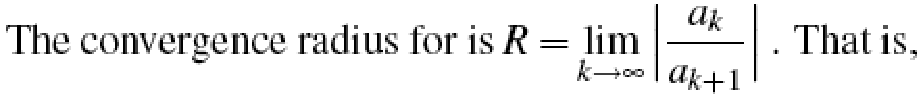
\includegraphics[width=0.55\textwidth]{latex}}}
\subfigure[由~Word软件生成的~.doc~格式行内公式]{\label{fig:subfig:word}
                \fbox{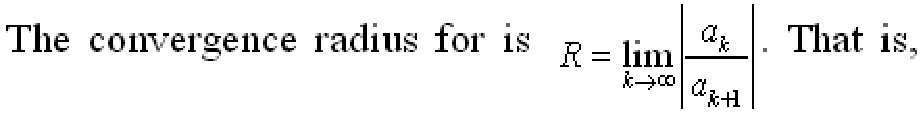
\includegraphics[width=0.55\textwidth]{word}}}
\subfigure[由~Word软件生成的~.pdf~格式行内公式]{\label{fig:subfig:pdf}
                \fbox{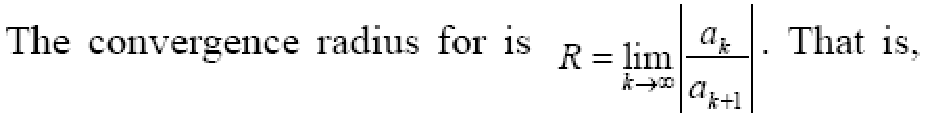
\includegraphics[width=0.55\textwidth]{pdf}}}

\caption{由~\LaTeX~和~Word~生成的~3~种行内公式屏显效果}\label{fig:hangju}
\vspace{-1em}
\end{figure}

这三幅图分别为~\LaTeX~和~Word~生成的行内公式屏显效果,从图中可看出,在~\LaTeX~文本含有公式的行内,在正文与公式之间对接工整,行距不变;而在~Word~文本含有公式的行内,在正文与公式之间对接不齐,行距变大。因此从这一点来说,
\LaTeX~系统在数学公式的排版上具有很大优势。

\LaTeX~提供的行内公式最简单、最有效的方法是采用~\TeX~本来的标记———开始和结束标记都写作~\$,例如本段开始的例子可由下面的输入得到。
\verb|$f(x)=\int_{a}^{b}\frac{\sin{x}}{x}\mathrm{d}x$|

\section{行间公式}
位于两行之间的公式称为行间公式,每个公式都是一个单独的段落,例如
\[\int_a^b{f\left(x\right)\mathrm{d}x}=\lim_{\left\|\Delta{x_i}\right\|\to 0}\sum_i{f\left(\xi_i\right)\Delta{x_i}}\]
除人工编号外,\LaTeX~各种类型行间公式的标记见表~\ref{tab:eqtag}。
\begin{table}[htbp]
\caption{各种类型行间公式的标记}\label{tab:eqtag}
\vspace{0.5em}\centering\wuhao
\begin{tabularx}{\textwidth}{cll}
\toprule
& 无编号 & 自动编号\\
\midrule
单行公式& \verb|\begin{displaymath}... \end{displaymath}|& \verb|\begin{equation}... \end{equation}|\\
        & 或~\verb|\[...\]| & \\
多行公式& \verb|\begin{eqnarray*}... \end{eqnarray*}|& \verb|\begin{eqnarray}... \end{eqnarray}|\\
\bottomrule
\end{tabularx}
\end{table}

另外,在自动编号的某行公式行尾添加标签~\verb|\nonumber|,可将该行转换为无编号形式。

行间多行公式需采用~\verb|eqnarray|~或~\verb|eqnarray*|~环境,它默认是一个列格式为~\verb|rcl|~的~3~列矩阵,并且中间列的字号要小一些,因此通常只将需要对齐的运算符号(通常为等号“=”)置于中间列。

\section{可自动调整大小的定界符}
若在左右两个定界符之前分别添加命令~\verb|\left|~和~\verb|\right|,则定界符可根据所包围公式大小自动调整其尺寸,这可从式(\ref{nodelimiter})和式(\ref{delimiter})中看出。
\begin{equation}\label{nodelimiter}
(\sum_{k=\frac12}^{N^2})
\end{equation}
\begin{equation}\label{delimiter}
\left(\sum_{k=\frac12}^{N^2}\right)
\end{equation}
式(\ref{nodelimiter})和式(\ref{delimiter})是在~\LaTeX~中分别输入如下代码得到的。
\begin{verbatim}
(\sum_{k=\frac12}^{N^2})
\left(\sum_{k=\frac12}^{N^2}\right)
\end{verbatim}
\verb|\left|~和~\verb|\right|~总是成对出现的,若只需在公式一侧有可自动调整大小的定界符,则只要用“.”代替另一侧那个无需打印出来的定界符即可。

若想获得关于此部分内容的更多信息,可参见~\href{http://tug.ctan.org/cgi-bin/ctanPackageInformation.py?id=voss-mathmode}{Math mode}~文档的第~8~章“Brackets, braces and parentheses”。

\section{数学重音符号}
数学重音符号通常用来区分同一字母表示的不同变量,输入方法如下(需要调用~\verb|amsmath|~宏包):

\vspace{0.5em}\noindent\wuhao\begin{tabularx}{\textwidth}{Xc|Xc|Xc}
 \verb|\acute| & $\acute{a}$ & \verb|\mathring| & $\mathring{a}$ & \verb|\underbrace| & $\underbrace{a}$ \\
 \verb|\bar| & $\bar{a}$ & \verb|\overbrace| & $\overbrace{a}$ & \verb|\underleftarrow| & $\underleftarrow{a}$ \\
 \verb|\breve| & $\breve{a}$ & \verb|\overleftarrow| & $\overleftarrow{a}$ & \verb|\underleftrightarrow| & $\underleftrightarrow{a}$ \\
 \verb|\check| & $\check{a}$ & \verb|\overleftrightarrow| & $\overleftrightarrow{a}$ & \verb|\underline| & $\underline{a}$ \\
 \verb|\dddot| & $\dddot{a}$ & \verb|\overline| & $\overline{a}$ & \verb|\underrightarrow| & $\underrightarrow{a}$ \\
 \verb|\ddot| & $\ddot{a}$ & \verb|\overrightarrow| & $\overrightarrow{a}$ & \verb|\vec| & $\vec{a}$ \\
 \verb|\dot| & $\dot{a}$ & \verb|\tilde| & $\tilde{a}$ & \verb|\widehat| & $\widehat{a}$ \\
 \verb|\grave| & $\grave{a}$ & \verb|\underbar| & $\underbar{a}$ & \verb|\widetilde| & $\widetilde{a}$ \\
 \verb|\hat| & $\hat{a}$
\end{tabularx}\vspace{0.5em}
\xiaosi 当需要在字母~$i$~和~$j$~的上方添加重音符号时,为了去掉这两个字母顶上的小点,这两个字母应该分别改用~\verb|\imath|~和~\verb|\jmath|。

如果遇到某些符号不知道该采用什么命令能输出它时,则可通过~\href{http://detexify.kirelabs.org/classify.html}{Detexify$^2$~网站}来获取符号命令。若用鼠标左键在此网页的方框区域内画出你所要找的符号形状,则会在网页右方列出和你所画符号形状相近的~5~个符号及其相对应的~\LaTeX~输入命令。若所列出的符号中不包括你所要找的符号,还可通过点击“Select from the complete list!”的链接以得分从低到高的顺序列出所有符号及其相对应的~\LaTeX~输入命令。

最后,建议大家还以~\href{http://tug.ctan.org/cgi-bin/ctanPackageInformation.py?id=voss-mathmode}{Math mode}~这篇~pdf~文档作为主要参考。若要获得最为标准、美观的数学公式排版形式,可以查查文档中是否有和你所要的排版形式相同或相近的代码段,通过修改代码段以获得你所要的数学公式排版形式。


% !Mode:: "TeX:UTF-8"

\chapter{罗列和定理环境使用方法}

\section{单层罗列环境}
湖南大学学位论文一般可采用两种罗列环境:一种是并列条目有同样标签的~\verb|itemize|~罗列环境,另一种是具有自动排序编号符号的~\verb|enumerate|~罗列环境。这两种罗列环境的样式参数可参考图~\ref{fig:list}。
\begin{figure}[htbp]
\centering
\includegraphics[width = 0.6\textwidth]{list}
\caption{罗列环境参数示意图}\label{fig:list}\vspace{-1em}
\end{figure}

通过调用~enumitem~宏包可以很方便地控制罗列环境的布局,其~format.tex~文件中的~\verb|\setitemize|~和~\verb|\setenumerate|~命令分别用来设置~\verb|itemize|~和~\verb|enumerate|~环境的样式参数。采用~\verb|itemize|~单层罗列环境的排版形式如下:

\begin{itemize}
\item 第一个条目文本内容
\item 第二个条目文本内容
\item 第三个条目文本内容
\end{itemize}

其代码如下

\begin{verbatim}
\begin{itemize}
  \item 第一个条目文本内容
  \item 第二个条目文本内容
  ...
  \item 第三个条目文本内容
\end{itemize}
\end{verbatim}

采用~\verb|enumerate|~单层罗列环境的排版形式如下:

\begin{enumerate}
\item 第一个条目文本内容
\item 第二个条目文本内容
\item 第三个条目文本内容
\end{enumerate}

其代码如下

\begin{verbatim}
\begin{enumerate}
  \item 第一个条目文本内容
  \item 第二个条目文本内容
  ...
  \item 第三个条目文本内容
\end{enumerate}
\end{verbatim}



\section{定理环境}

\begin{definition}[谱半径]\label{def:def1}
  称~$n$~阶方阵~$\mathbf{A}$~的全体特征值~$\lambda_1,\cdots,\lambda_n$~组成的集合为~$\mathbf{A}$~的谱,称
  $$\rho(\mathbf{A})=\max{\{|\lambda_1|,\cdots,|\lambda_n|\}}$$
\end{definition}
\begin{theorem}[相似充要条件]\label{lemma:l1}
  方阵$A$和$B$相似的充要条件是:~$A$~和~$B$~有全同的不变因子。
\end{theorem}
\begin{corollary}[推论1]\label{cor:cor1}
在赋范空间~$(X,\|\cdot\|)$~上定义~$d(x,y)=\|x-y\|$, 对任意~$x,y\in X$,~则~$(X,d)$~是距离空间。
\end{corollary}
\begin{proof}
  只需证明~$d(x,y)$~是距离。
\end{proof}
\newpage

定义代码如下:
\begin{verbatim}
 \begin{definition}[谱半径]\label{def:def1}
  称~$n$~阶方阵~$\mathbf{A}$~的全体特征值
  $\lambda_1,\cdots,\lambda_n$组成的集合为~$\mathbf{A}$~的谱,称
  $$\rho(\mathbf{A})=\max{\{|\lambda_1|,\cdots,|\lambda_n|\}}$$
\end{definition}
\end{verbatim}
\noindent\hrule

\vspace{0.1em}\noindent\hrule
\vspace{1em}
定理代码如下:
\begin{verbatim}
\begin{theorem}[相似充要条件]\label{lemma:l1}
  方阵$A$和$B$相似的充要条件是:$A$和$B$有全同的不变因子。
\end{theorem}
\end{verbatim}
\noindent\hrule\vspace{0.1em}

\noindent\hrule
\vspace{1em}
推论和证明代码如下:
\begin{verbatim}
\begin{corollary}[推论1]\label{cor:cor1}
在赋范空间~$(X,\|\cdot\|)$~上定义$d(x,y)=\|x-y\|$,
对任意$x,y\in X$,则$(X,d)$是距离空间。
\end{corollary}
\begin{proof}
  只需证明$d(x,y)$是距离。
\end{proof}
\end{verbatim}
\noindent\hrule\vspace{1em}

定理定义[]中是可选参数,用来说明定理的名称。其他环境格式书写与上面定理、定义、推论格式相同,可自己调用其他环境。
若需要书写定理定义等内容,而且带有顺序编号,需要采用如下环境。除了~\verb|proof|~环境之外,其余~9~个环境都可以有一个可选参数作为附加标题。

\begin{center}
\vspace{0.5em}\noindent\wuhao\begin{tabularx}{0.7\textwidth}{lX|lX}
定理 & \verb|theorem|~环境 & 定义 & \verb|definition|~环境 \\
例 & \verb|example|~环境 & 算法 & \verb|algorithm|~环境 \\
公理 & \verb|axiom|~环境 & 命题 & \verb|proposition|~环境 \\
引理 & \verb|lemma|~环境 & 推论 & \verb|corollary|~环境 \\
注解 & \verb|remark|~环境 & 证明 & \verb|proof|~环境 \\
\end{tabularx}
\end{center} 
% !Mode:: "TeX:UTF-8"

\addcontentsline{toc}{chapter}{结\quad 论} %添加到目录中
\chapter*{结\quad 论}

本文在分析分布式图处理系统和单机图处理系统的基础上,对目前图处理系统中的一些缺陷进行讨论,并在传统BSP计算模型的基础上,利用Actor并发模型对BSP模型进行优化,提出了基于Actor并发模型的BSP计算模型。通过对Actor-BSP模型的数据行为进行分析和讨论,将图数据分为两个部分:常驻内存的顶点状态信息和保存在磁盘上的边数据信息,同时利用内存映射优化IO操作。实验证明,GPSA图处理系统不仅能够在单机多核系统上高效的处理大规模图,同时还能够充分发挥多核的优势。本文的主要工作包括以下几个方面:

1、本论文在做了大量调研的基础上,对目前大规模图处理系统进行分析和对比,详细讨论目前存在于分布式图处理系统的困难问题,说明在单机系统上进行大规模图处理的可行性,对单机系统上的图处理系统进行分析和对比,从计算模型的角度出发,对传统的BSP模型进行优化,提出崭新的Actor-BSP图计算模型。Actor-BSP模型中将传统以顶点为中心的模型中顺序执行的计算过程和分发过程分离解耦,同时使用Actor代替线程,并将计算过程和分发过程分布在不同的Actor上,提高任务并发量。同时,Actor-BSP简化了图计算的流程,由于淡化顶点作为整个计算的中心的概念,顶点之间消息的传递转换为Actor之间的消息分发,计算过程和分发过程之间通过消息建立联系,从而无需再计算中缓存大量的消息,节省大量的IO操作。另外,Actor-BSP模型缩短了单个任务的平均执行时间,提升计算效率。

2、在Actor-BSP模型的基础上对数据的访问行为进行分析和讨论,由于新模型消息发送的随机性,就无法避免计算Actor对顶点状态信息的随机访问,与其他单机系统尽力回避随机访问的做法不同,GPSA大胆的采用数据分离的方法,将图数据分为两个独立的部分:顶点的状态信息和图的结构信息。其中,顶点的状态信息按照顺序存储的方式利用内存映射技术将其映射到内存来支持随机访问,提升效率。而对于图的结构信息则保持于磁盘上,可以采用顺序访问的方式,进一步节省IO操作。


3.独立完成了本文所论述的GPSA系统的调研,方案设计,具体编码实现和测试工作。列举PageRank、连通分量以及广度优先搜索三个常见图应用在GPSA系统上的实现,并将之与其他单机图处理系统从效率和多核利用率两个方面进行对比和分析,结果表明,GPSA不仅具有高效能够充分发挥多核优势的特点,而且具有较好的伸缩性与容错性。

虽然GPSA从改进计算模型角度出发,并取得良好的效果,但是GPSA依然存在一些不足,有待进一步完善。

首先,GPSA不支持图结构改变的应用。GPSA将图分为两部分:顶点信息和边。其中,顶点常驻内存,支持随机访问和更新,但是边、边上的权重等信息保存在磁盘上,需要尽量避免随机读写。

其次,GPSA使用JAVA实现,在实现过程中为避免频繁的垃圾回收造成的性能影响,在消息的封装中使用基本类型,造成消息的生成仅仅支持数字类型,无法支持字符串或者对象等。

最后,GPSA的设计初衷是能够兼容分布式以BSP为计算模型的大规模图处理系统,但是由于时间、经济等方面条件限制,该部分猜想的验证无力完成,希望能在将来能继续进行并开展在分布式方向的扩展和实验。

%%%%%%%%%% 正文部分内容  %%%%%%%%%%

%%%%%%%%%%  参考文献  %%%%%%%%%%
\defaultfont
\bibliographystyle{HNUThesis}
\phantomsection
\addcontentsline{toc}{chapter}{参考文献}          % 参考文献加入到中文目录
\nocite{*}                                        % 若将此命令屏蔽掉,则未引用的文献不会出现在文后的参考文献中。
\bibliography{reference}
% !Mode:: "TeX:UTF-8"
\addcontentsline{toc}{chapter}{致\quad 谢} %添加到目录中
\chapter*{致\quad 谢}


三年的研究生生活即将结束,我首先要感谢我的导师陈浩教授,本论文的完成得益于他的悉心指导和无倦教诲,论文从选题、构思、一直到修改都倾注了导师大量心血。陈老师严谨的治学态度、渊博的学识、博大的胸襟、一丝不苟的工作作风和平易近人的性格,都给我留下了深刻的印象。另外还要感谢孙建华副教授,她敏锐的洞察力以及对学术研究的极大热情令人敬佩。两位老师提倡的学术自由极大的激发了我们的研究热情和创新欲望,使我的科研水平以及综合素质得到提高。在论文完成之际,特向他们致以诚挚的敬意和衷心的感谢。

在论文的创作中还得到了许多同学的倾心帮助。常诚师兄在论文工作中给予了大量帮助、指导和有益讨论,促使我在学术上不断进步。谭元元、佘玲军等同学作为实验室的小伙伴在业余时间相互探讨也给了我不少启迪,开阔了我的写作思路。师弟师妹们以及室友也给予了大量的帮助和支持,让我度过了一段难忘的时光,在此一并感谢,并祝你们成功! 
特别地,我要感谢我的家人,他们总是在背后默默的支持着我,一直记挂我的身体和学业,是他们给了我无穷的力量,让我迎接挑战,不断进步,祝福他们快乐,安康! 

我还要感谢本论文所引文献的全部作者及所有为这篇论文做出贡献的人。

由于本人学术水平有限,论文中如有不妥之处,敬请各位老师批评、指正。最后,谨向在百忙之中抽出宝贵时间审阅本论文及答辩组的老师们致以最诚挚的谢意!

               % 致谢
% !Mode:: "TeX:UTF-8"

\addcontentsline{toc}{chapter}{附录A  发表论文和参加科研情况说明}
\chapter*{附录A~~~~发表论文和参加科研情况说明}
\setlength{\parindent}{0em}
\textbf{(一)发表的学术论文}
\begin{publist}
	\item XXX,XXX. GPSA: a Graph Processing System With Actors. ICPP 2015,已录用,待发表
\end{publist}

\vspace*{1em}

\textbf{(二)参与的科研项目}
\begin{publist}
\item 国家自然科学基金,基于程序分析方法的Web安全研究(61173166),2012.1-2015.12

\item 国家自然科学基金,GPU通用计算系统检查点方法研究(61272190),2013.1-2016.12

\item 新世纪优秀人才支持计划,基于多核不对称特性的虚拟机优化方法研究, 2013.1-2015.12
\end{publist}
\vfill
\hangafter=1\hangindent=2em\noindent

\setlength{\parindent}{2em}
                   % 发表论文和参加科研情况说明
\clearpage
\end{CJK*}                                        % 结束中文字体使用
\end{document}                                    % 结束全文
